\newpage
\begin{appendix}
\chapter{Detailed Evaluation of DVS Data Sets}
A thorough evaluation of the influence of different parameter settings has been conducted. Following tables list all conducted evaluations for the three real-life ground truth data sets.


\begin{table}[tb]
	\centering
		\begin{tabular}{lccc}
Setting & Filter Length [ms] & Temp. Res. [ms] & Angle incr. ($0$ to $360^\circ$) \\
\hline  \hline
R$1$ & $0.70$ & $0.010$ & $45.00$\\
R$2$ & $0.70$ & $0.010$ & $30.00$\\
R$5$ & $0.30$ & $0.010$ & $45.00$\\
R$6$ & $0.30$ & $0.010$ & $30.00$\\
R$3$ & $0.50$ & $0.010$ & $45.00$\\
R$4$ & $0.50$ & $0.010$ & $30.00$\\
R$7$ & $0.30$ & $0.005$ & $45.00$\\
R$8$ & $0.30$ & $0.005$ & $30.00$\\
R$9$ & $0.50$ & $0.005$ & $45.00$\\
R$10$ & $0.50$ & $0.005$ & $30.00$\\
R$11$ & $0.70$ & $0.005$ & $45.00$\\
R$12$ & $0.70$ & $0.005$ & $30.00$\\
		\end{tabular}
	\caption[Different parameter settings for the evaluations]{Different parameter settings have been used for the evaluation of the flow.
	 The spatial size of the filter remained constant during the experiments.
	 The filter length was adjusted as well as the temporal resolution, i.e. the distance between time slices. 
	 Furthermore, the composition of the filter bank was varied by changing the rotation of the individual Gabor filters. 
	 For this, Gabor filters were rotated by angles between $0$ and $360$ degrees with constant angular increments.}
	\label{tab:app_parameter_settings}
\end{table}



\begin{table}[tb]
	\centering
		\begin{tabular}{lccccccc}
Scene & Setting & Matching & RMSE & MeanErr & MedianErr & Avg. Angle \\
\hline  \hline
quadrat & R$1$ & direct & $19.58$ & $11.66$ & $6.19$ & $1.29$ & \\
quadrat & R$1$ & interp & $20.93$ & $12.61$ & $6.53$ &  & \\
quadrat & R$2$ & direct & $19.21$ & $11.36$ & $6.19$ & $1.31$ & \\
quadrat & R$2$ & interp & $20.69$ & $12.45$ & $6.75$ &  & \\
quadrat & R$3$ & direct & $22.41$ & $11.04$ & $4.89$ & $1.12$ & \\
quadrat & R$3$ & interp & $22.48$ & $11.14$ & $4.91$ &  & \\
quadrat & R$4$ & direct & $21.84$ & $10.85$ & $4.96$ & $1.16$ & \\
quadrat & R$4$ & interp & $21.82$ & $10.96$ & $4.97$ &  & \\
quadrat & R$5$ & direct & $33.70$ & $15.10$ & $5.13$ & $1.15$ & \\
quadrat & R$5$ & interp & $33.79$ & $15.26$ & $5.09$ &  & \\
quadrat & R$6$ & direct & $33.48$ & $15.04$ & $5.20$ & $1.23$ & \\
quadrat & R$6$ & interp & $33.57$ & $15.21$ & $5.16$ &  & \\
quadrat & R$7$ & direct & $32.76$ & $15.46$ & $5.37$ & $1.18$ & \\
quadrat & R$7$ & interp & $33.19$ & $15.75$ & $5.35$ &  & \\
quadrat & R$8$ & direct & $32.53$ & $15.39$ & $5.43$ & $1.29$ & \\
quadrat & R$8$ & interp & $32.96$ & $15.68$ & $5.43$ &  & \\
quadrat & R$9$ & direct & $21.84$ & $11.14$ & $4.92$ & $1.12$ & \\
quadrat & R$9$ & interp & $22.55$ & $11.44$ & $4.92$ &  & \\
quadrat & R$10$ & direct & $21.60$ & $11.03$ & $4.93$ & $1.17$ & \\
quadrat & R$10$ & interp & $22.32$ & $11.36$ & $4.97$ &  & \\
quadrat & R$11$ & direct & $16.33$ & $10.38$ & $6.24$ & $1.21$ & \\
quadrat & R$11$ & interp & $17.12$ & $10.81$ & $6.48$ &  & \\
quadrat & R$12$ & direct & $15.99$ & $10.17$ & $6.26$ & $1.26$ & \\
quadrat & R$12$ & interp & $16.86$ & $10.72$ & $6.62$ &  & \\
		\end{tabular}
	\caption[First scene: Comparison of angular errors for different parameters.]{Comparison of angular errors for the moving square scene.
	The Setting attribute describes the composition of the temporal filter length as well as temporal resolution.
	 These settings can be compared in table \ref{tab:parameter_settings}. Considering the provided ground truth, parameter combination 3 lead to the lowest median error. When considering the underlying scene with vertical edges moving in $x$-direction, the average angle in setting 5 points to even better results.}
	\label{tab:app_error_comparison_quadrat}
	 \end{table}
	 
	 \begin{table}[tb]
	\centering
		\begin{tabular}{lccccccc}
Scene & Setting & Matching & RMSE & MeanErr & MedianErr & Avg. Angle \\
\hline  \hline
pushbot & R$1$ & direct & $94.05$ & $78.66$ & $71.46$ & -$101.32$ & \\
pushbot & R$1$ & interp & $94.34$ & $78.96$ & $71.96$ &  & \\
pushbot & R$2$ & direct & $94.12$ & $78.69$ & $71.32$ & -$101.33$ & \\
pushbot & R$2$ & interp & $94.35$ & $78.96$ & $71.98$ &  & \\
pushbot & R$3$ & direct & $92.84$ & $76.28$ & $66.58$ & -$103.75$ & \\
pushbot & R$3$ & interp & $93.43$ & $76.85$ & $67.59$ &  & \\
pushbot & R$4$ & direct & $92.79$ & $76.23$ & $66.73$ & -$103.29$ & \\
pushbot & R$4$ & interp & $93.39$ & $76.80$ & $67.87$ &  & \\
pushbot & R$5$ & direct & $94.54$ & $78.14$ & $69.79$ & -$101.37$ & \\
pushbot & R$5$ & interp & $95.22$ & $78.85$ & $70.87$ &  & \\
pushbot & R$6$ & direct & $94.54$ & $78.13$ & $69.83$ & -$101.27$ & \\
pushbot & R$6$ & interp & $95.23$ & $78.87$ & $70.97$ &  & \\
pushbot & R$7$ & direct & $93.73$ & $77.22$ & $68.16$ & -$99.43$ & \\
pushbot & R$7$ & interp & $94.69$ & $78.23$ & $69.74$ &  & \\
pushbot & R$8$ & direct & $93.74$ & $77.22$ & $68.27$ & -$99.06$ & \\
pushbot & R$8$ & interp & $94.72$ & $78.26$ & $69.90$ &  & \\
pushbot & R$9$ & direct & $91.69$ & $74.93$ & $64.18$ & -$102.94$ & \\
pushbot & R$9$ & interp & $92.62$ & $75.91$ & $65.97$ &  & \\
pushbot & R$10$ & direct & $91.66$ & $74.89$ & $64.03$ & -$102.48$ & \\
pushbot & R$10$ & interp & $92.56$ & $75.84$ & $65.61$ &  & \\
pushbot & R$11$ & direct & $92.64$ & $77.16$ & $69.08$ & -$100.00$ & \\
pushbot & R$11$ & interp & $93.39$ & $77.89$ & $70.17$ &  & \\
pushbot & R$12$ & direct & $92.71$ & $77.18$ & $69.12$ & -$99.99$ & \\
pushbot & R$12$ & interp & $93.41$ & $77.89$ & $70.33$ &  & \\
		\end{tabular}
	\caption[Second scene: Comparison of angular errors for different parameters.]{Second scene: Comparison of angular errors for different parameters. The algorithm could not properly compute the flow for movement that is not perpendicular to the object's edges. This leads to a rather high angular error for all settings.}
	\label{tab:app_error_comparison_pushbot}
\end{table}


\begin{table}[tb]
	\centering
		\begin{tabular}{lccccccc}
Scene & Setting & Matching & RMSE & MeanErr & MedianErr & Avg. Angle \\
\hline  \hline
skateboard & R$1$ & direct & $91.93$ & $73.85$ & $61.86$ & $58.94$ & \\
skateboard & R$1$ & interp & $91.75$ & $73.47$ & $60.94$ &  & \\
skateboard & R$2$ & direct & $91.78$ & $73.75$ & $61.77$ & $58.37$ & \\
skateboard & R$2$ & interp & $91.58$ & $73.36$ & $61.02$ &  & \\
skateboard & R$3$ & direct & $90.76$ & $72.70$ & $59.52$ & -$25.82$ & \\
skateboard & R$3$ & interp & $90.38$ & $72.16$ & $58.44$ &  & \\
skateboard & R$4$ & direct & $90.95$ & $73.07$ & $60.28$ & -$13.33$ & \\
skateboard & R$4$ & interp & $90.60$ & $72.54$ & $59.14$ &  & \\
skateboard & R$5$ & direct & $93.29$ & $75.56$ & $64.11$ & -$58.31$ & \\
skateboard & R$5$ & interp & $92.90$ & $74.98$ & $62.95$ &  & \\
skateboard & R$6$ & direct & $93.37$ & $75.82$ & $64.66$ & -$53.51$ & \\
skateboard & R$6$ & interp & $93.01$ & $75.27$ & $63.60$ &  & \\
skateboard & R$7$ & direct & $93.08$ & $75.39$ & $64.09$ & -$59.19$ & \\
skateboard & R$7$ & interp & $92.65$ & $74.78$ & $62.82$ &  & \\
skateboard & R$8$ & direct & $93.14$ & $75.63$ & $64.59$ & -$53.95$ & \\
skateboard & R$8$ & interp & $92.73$ & $75.04$ & $63.33$ &  & \\
skateboard & R$9$ & direct & $90.87$ & $72.91$ & $59.92$ & -$14.68$ & \\
skateboard & R$9$ & interp & $90.46$ & $72.35$ & $58.71$ &  & \\
skateboard & R$10$ & direct & $91.06$ & $73.28$ & $60.82$ & $2.49$ & \\
skateboard & R$10$ & interp & $90.69$ & $72.73$ & $59.71$ &  & \\
skateboard & R$11$ & direct & $92.06$ & $74.18$ & $62.78$ & $64.44$ & \\
skateboard & R$11$ & interp & $91.92$ & $73.85$ & $61.97$ &  & \\
skateboard & R$12$ & direct & $91.91$ & $74.09$ & $62.62$ & $64.99$ & \\
skateboard & R$12$ & interp & $91.77$ & $73.75$ & $61.84$ &  & \\
		\end{tabular}
	\caption[Third scene: Comparison of angular errors for different parameters.]{Third scene: Comparison of angular errors for different parameters. 
	Due to a high degree of noise, the angular error is rather high and the average angle greatly varies.}
	\label{tab:app_error_comparison_skateboard}
\end{table}

\chapter{Visualization of temporal Changes in the flow field}
Following figures show two subsequent frames of the optic flow generated by our algorithm as well as the ground truth.
To emphasize the event locations, we applied the previously described masks again.

\begin{figure}[tb]
\centering
\begin{subfigure}{.45\textwidth}
  \centering
  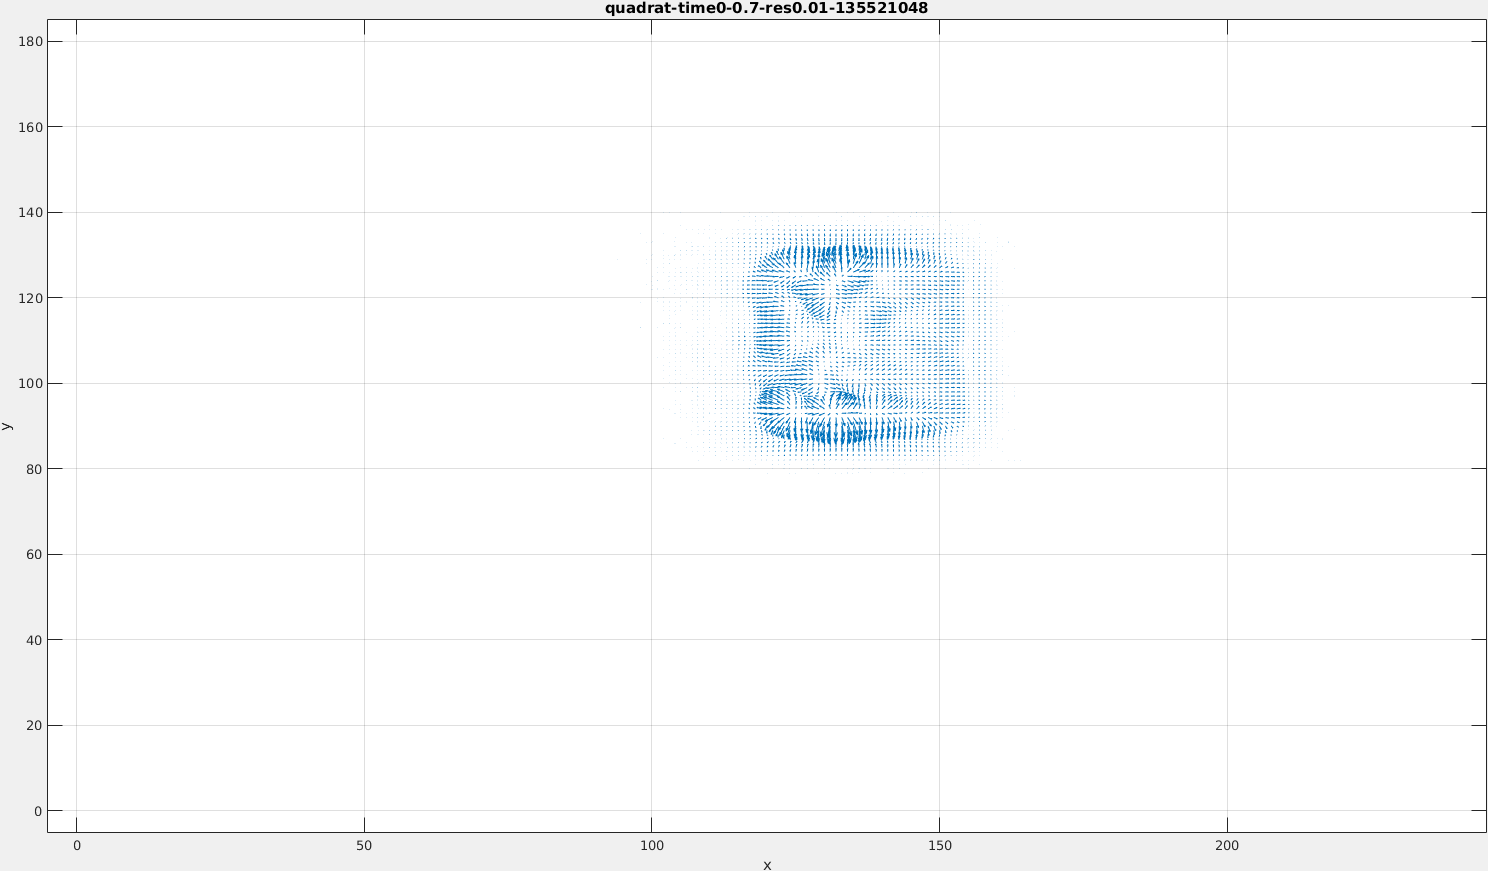
\includegraphics[height=.6\linewidth]{figs/quadrat/quadrat-1.png}
  \caption{}
\end{subfigure}
\begin{subfigure}{.45\textwidth}
  \centering
  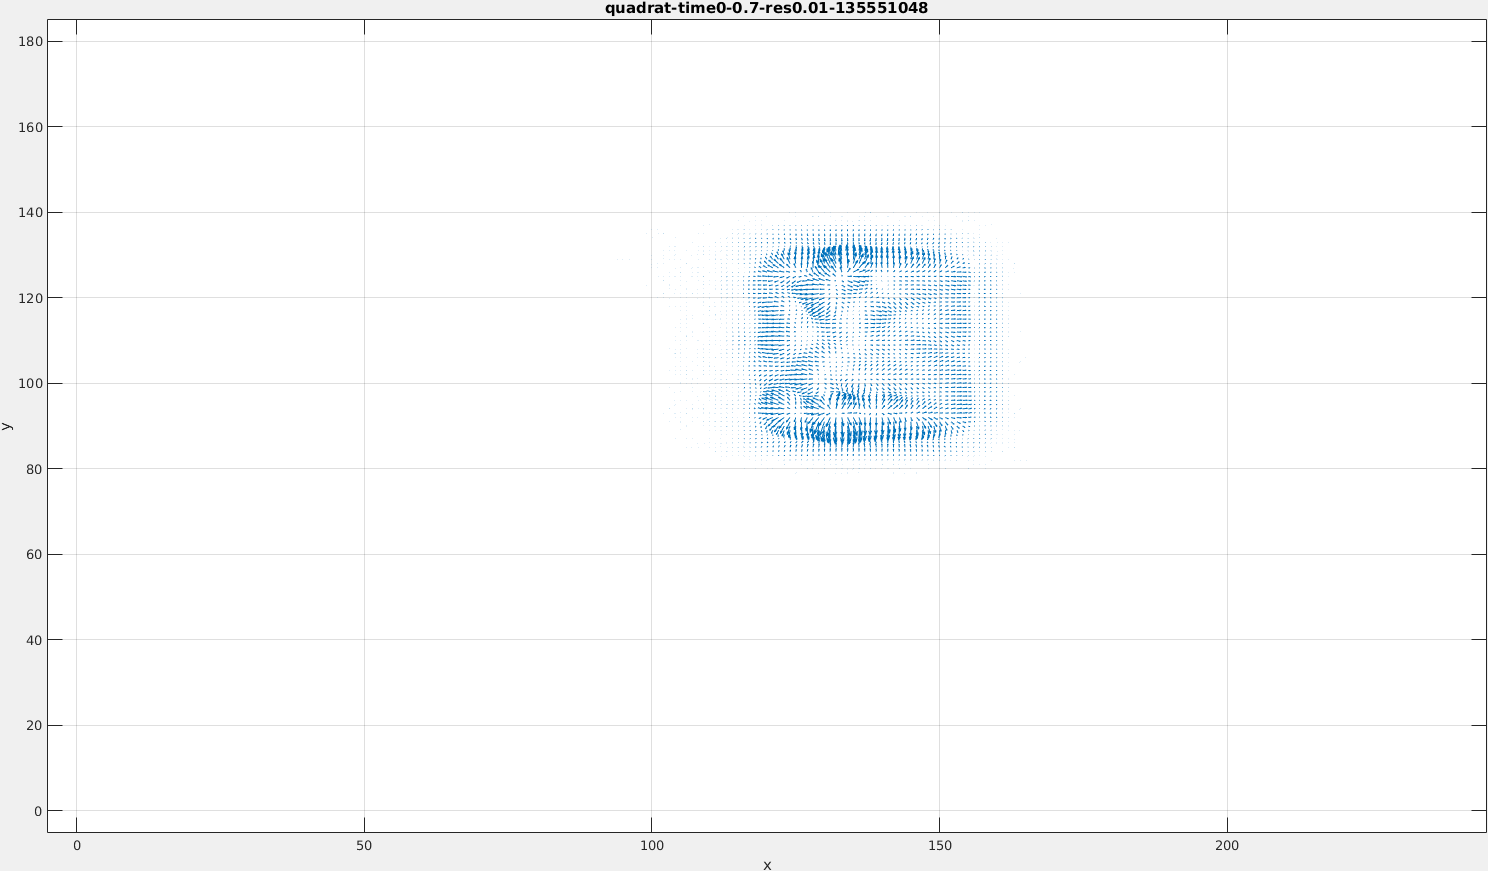
\includegraphics[height=.6\linewidth]{figs/quadrat/quadrat-2.png}
  \caption{}
\end{subfigure}
\begin{subfigure}{.45\textwidth}
  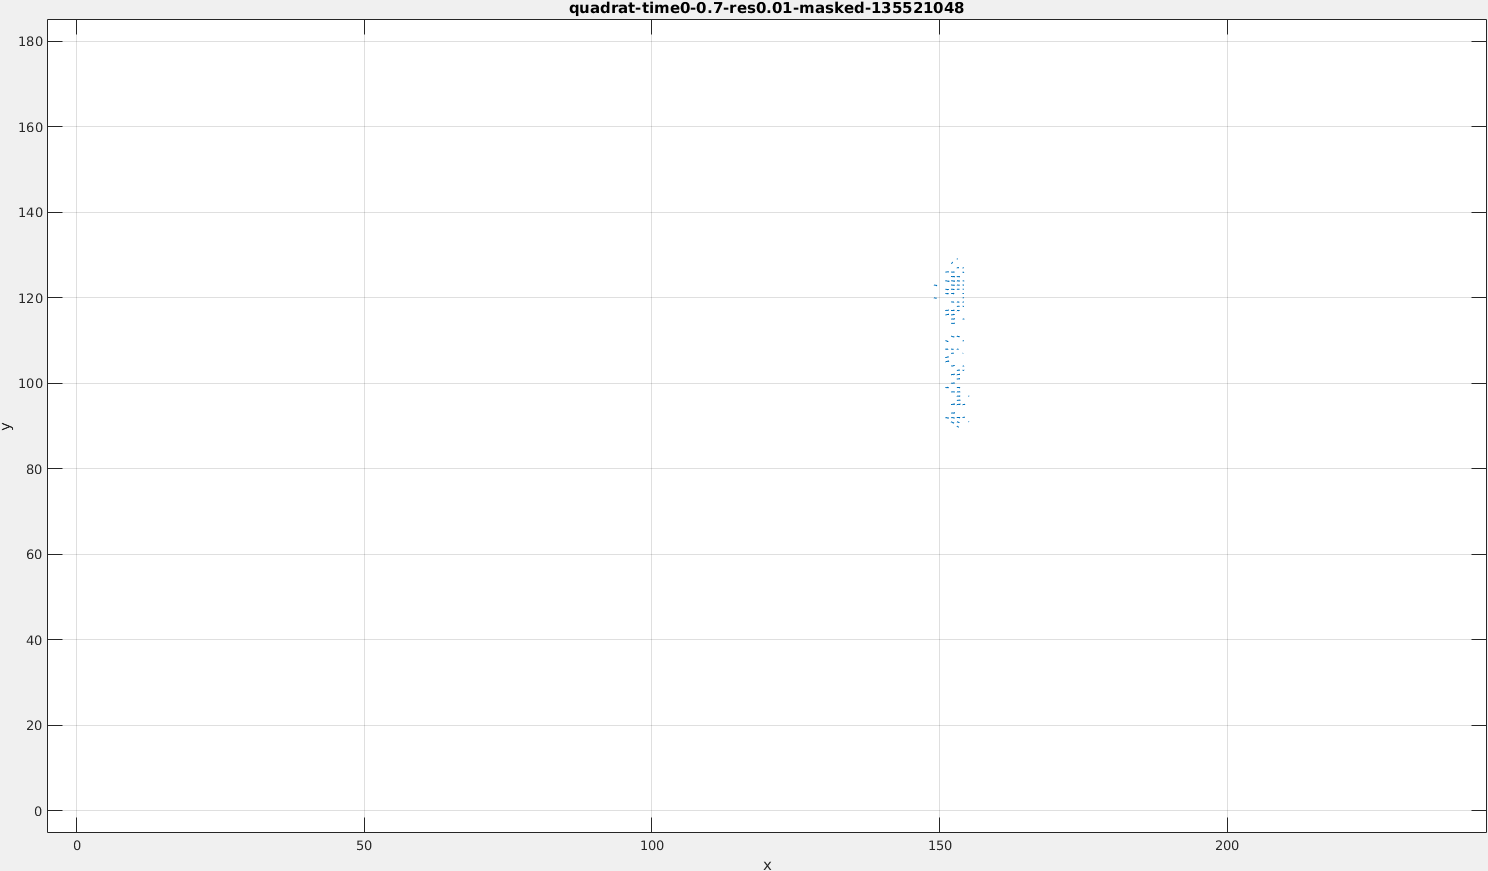
\includegraphics[height=.6\linewidth]{figs/quadrat/quadrat-masked-1.png}
  \caption{}
\end{subfigure}
\begin{subfigure}{.45\textwidth}
  \centering
  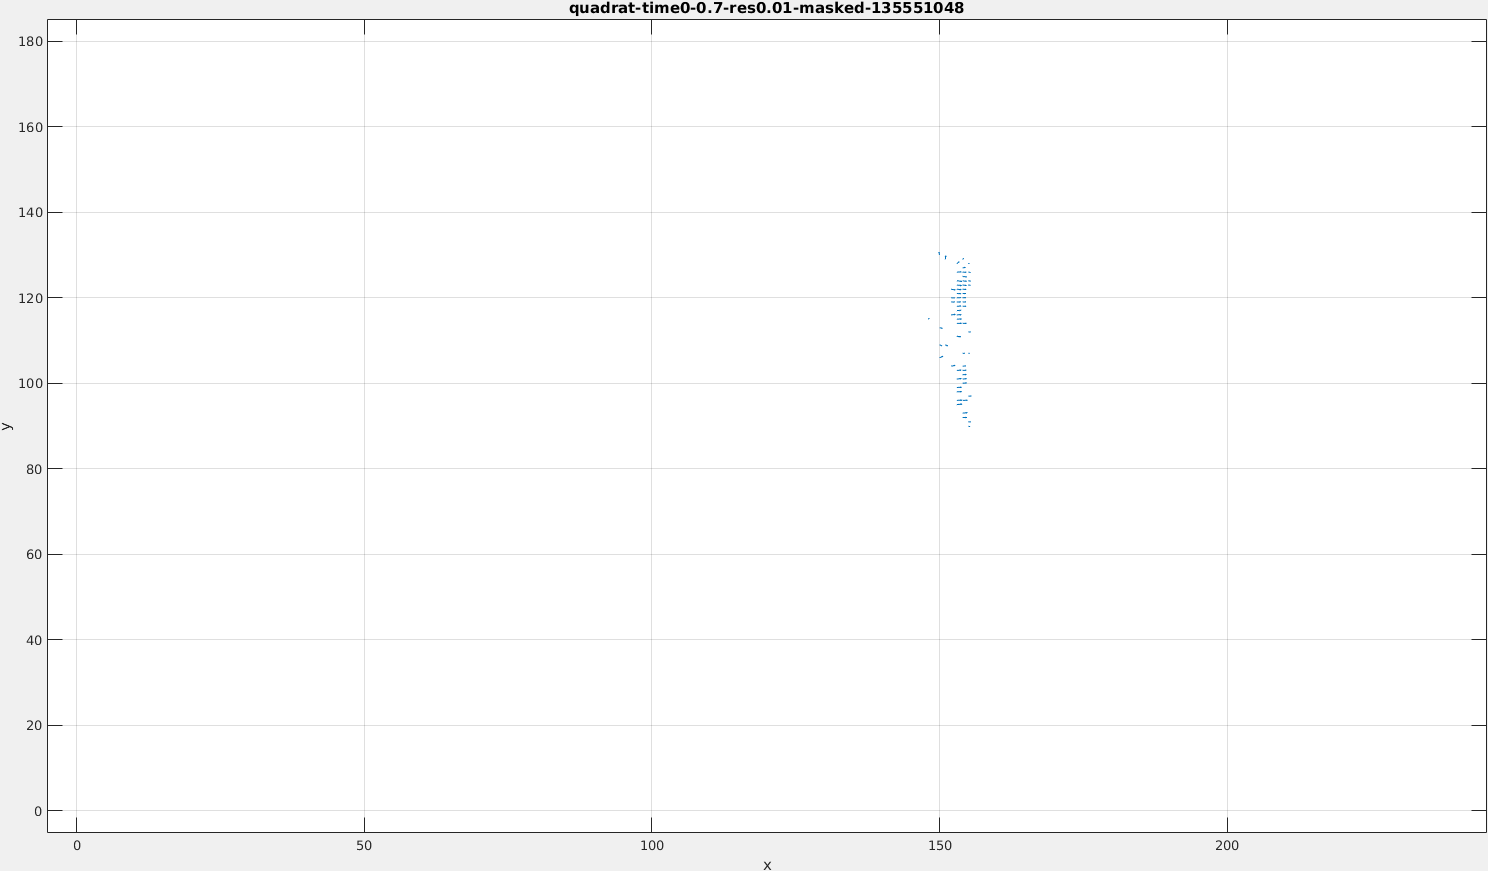
\includegraphics[height=.6\linewidth]{figs/quadrat/quadrat-masked-2.png}
  \caption{}
\end{subfigure}
\begin{subfigure}{.45\textwidth}
  \centering
  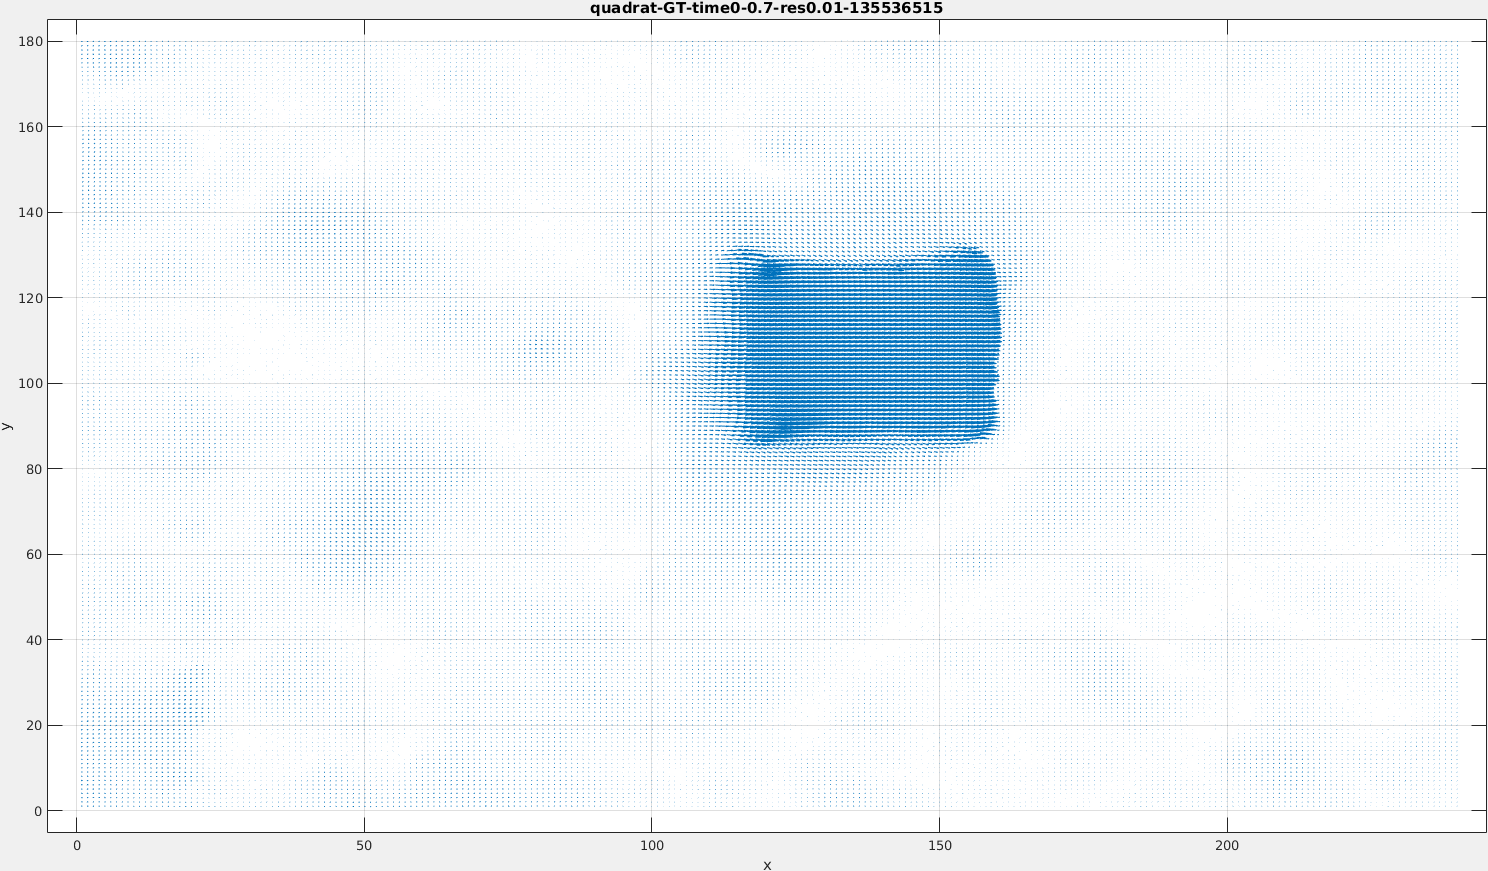
\includegraphics[height=.6\linewidth]{figs/quadrat/quadrat-GT-1.png}
  \caption{}
\end{subfigure}
\begin{subfigure}{.45\textwidth}
  \centering
  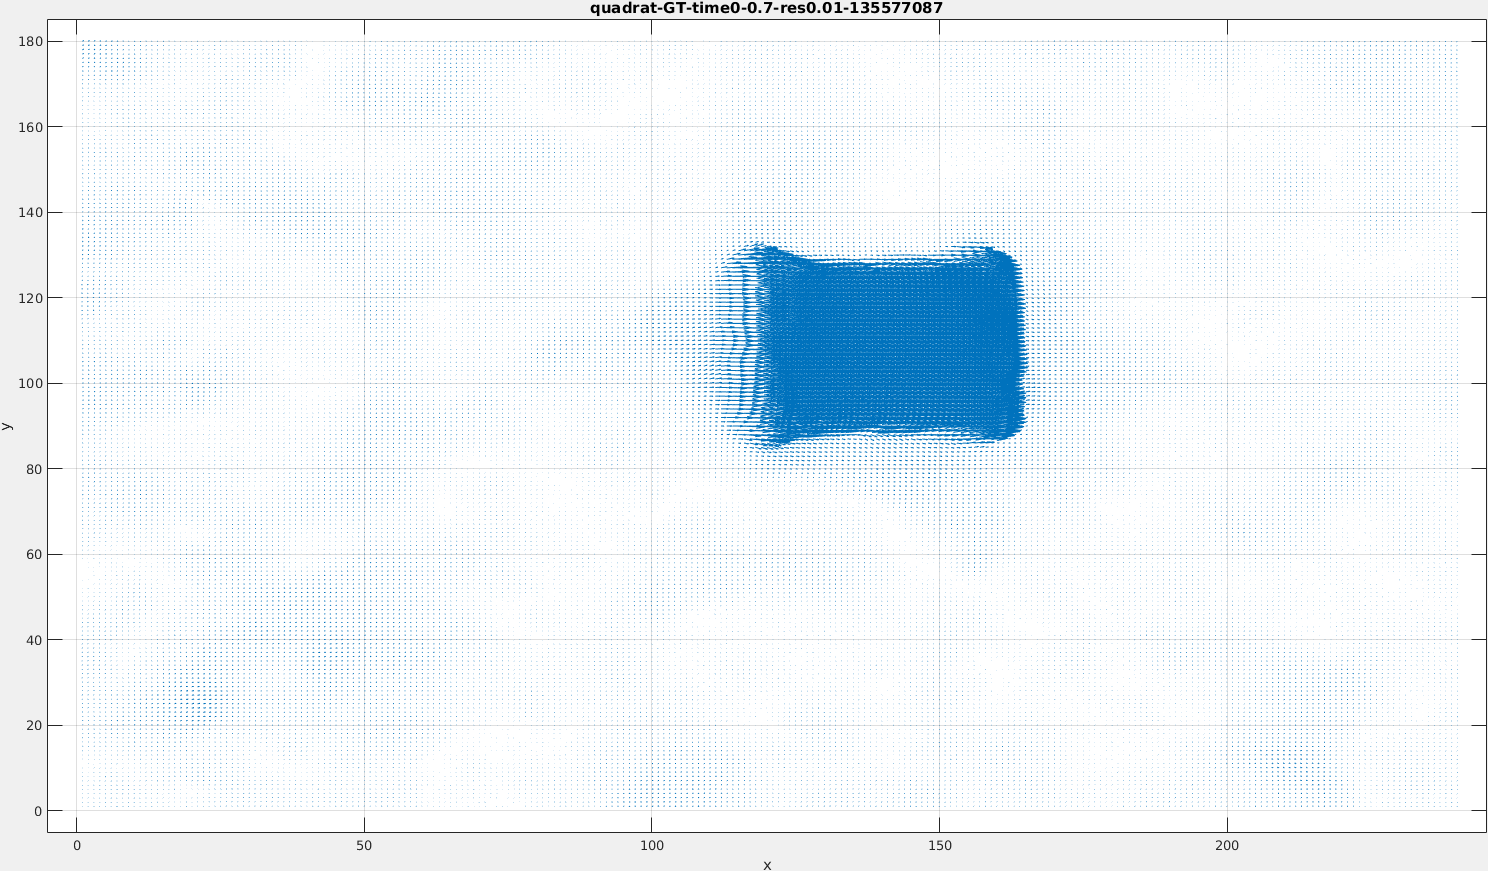
\includegraphics[height=.6\linewidth]{figs/quadrat/quadrat-GT-2.png}
  \caption{}
\end{subfigure}
\begin{subfigure}{.45\textwidth}
  \centering
  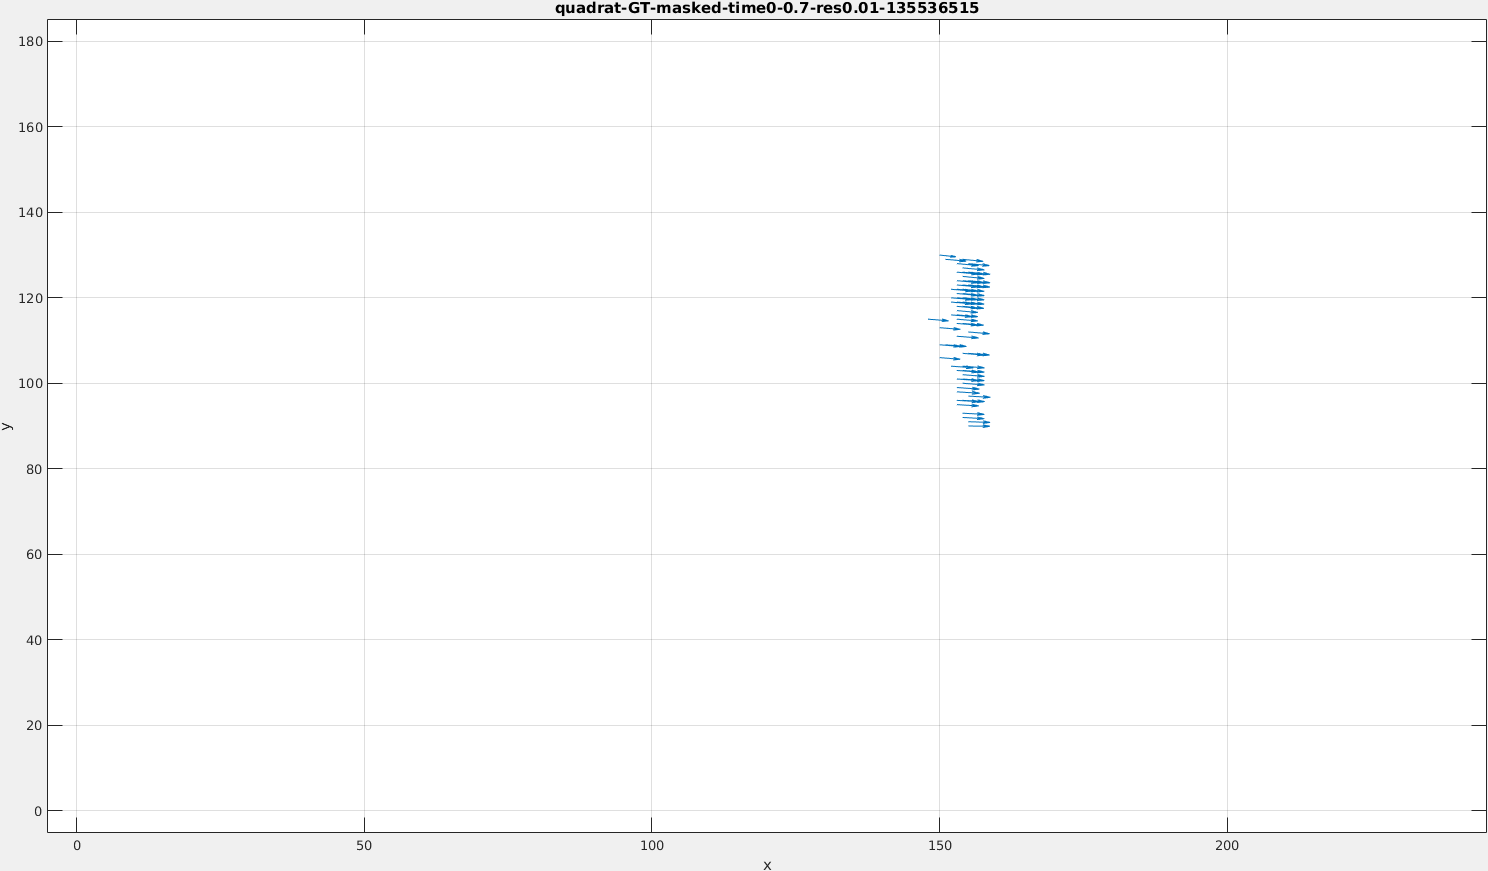
\includegraphics[height=.6\linewidth]{figs/quadrat/quadrat-GT-masked-1.png}
  \caption{}
\end{subfigure}
\begin{subfigure}{.45\textwidth}
  \centering
  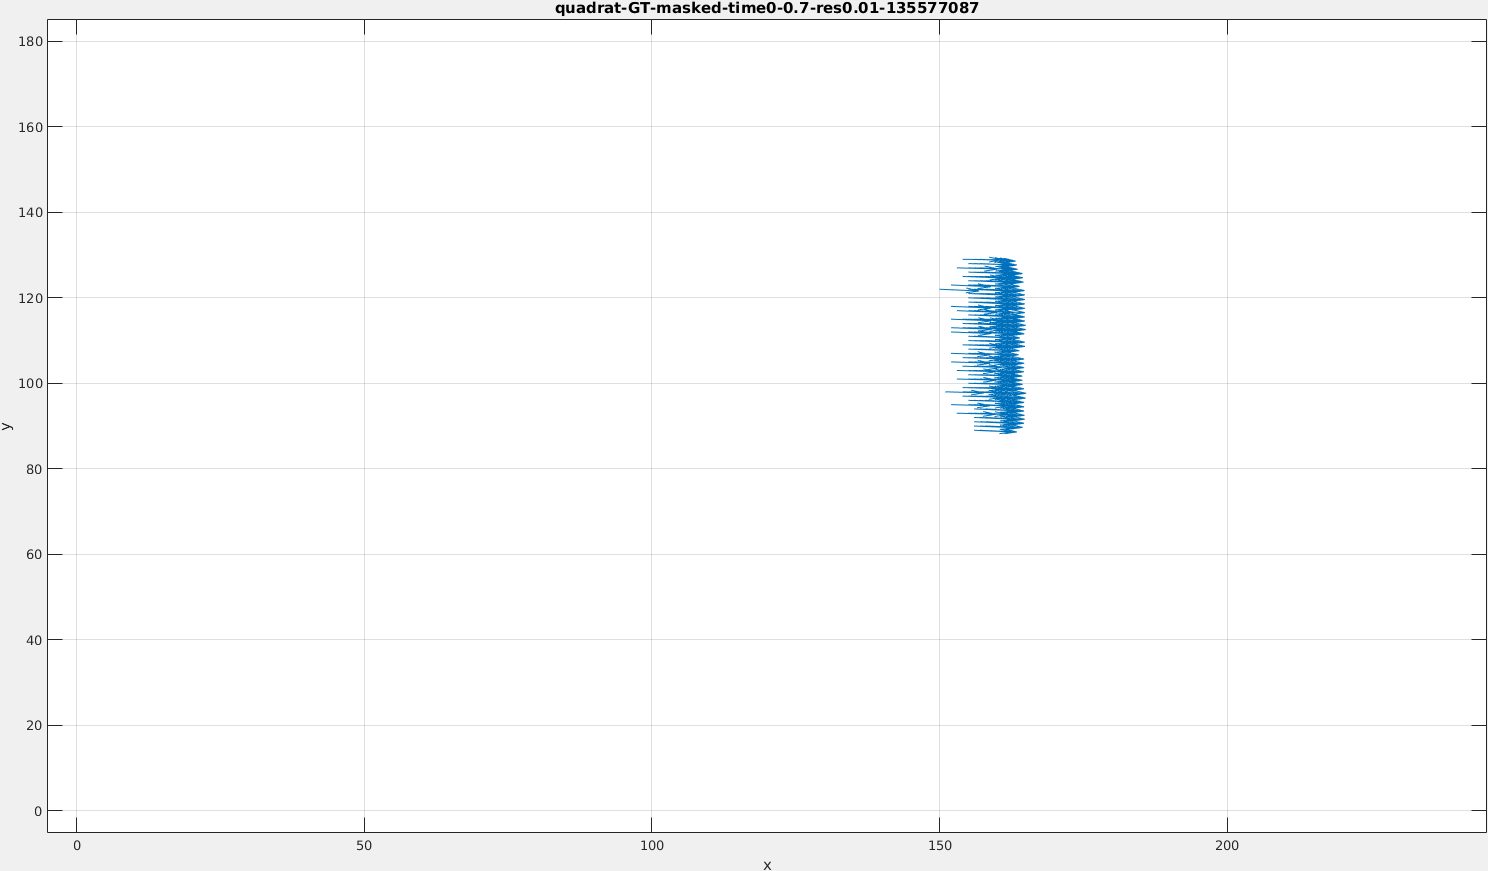
\includegraphics[height=.6\linewidth]{figs/quadrat/quadrat-GT-masked-2.png}
  \caption{}
\end{subfigure}
\caption[First scene: Robot approaching the DVS sensor.]{Second scene: Robot approaching the DVS sensor.
Figures (a) and (b) show the computed optical flow for the scene at two time steps. The masked flow fields are shown in Figures (c) and (d).
The corresponding ground truth is shown in Figures (e) and (f). Applying the same mask leads to Figures (g) and (h)}
\label{fig:app_quadrat-snapshots}
\end{figure}



\begin{figure}[tb]
\centering
\begin{subfigure}{.45\textwidth}
  \centering
  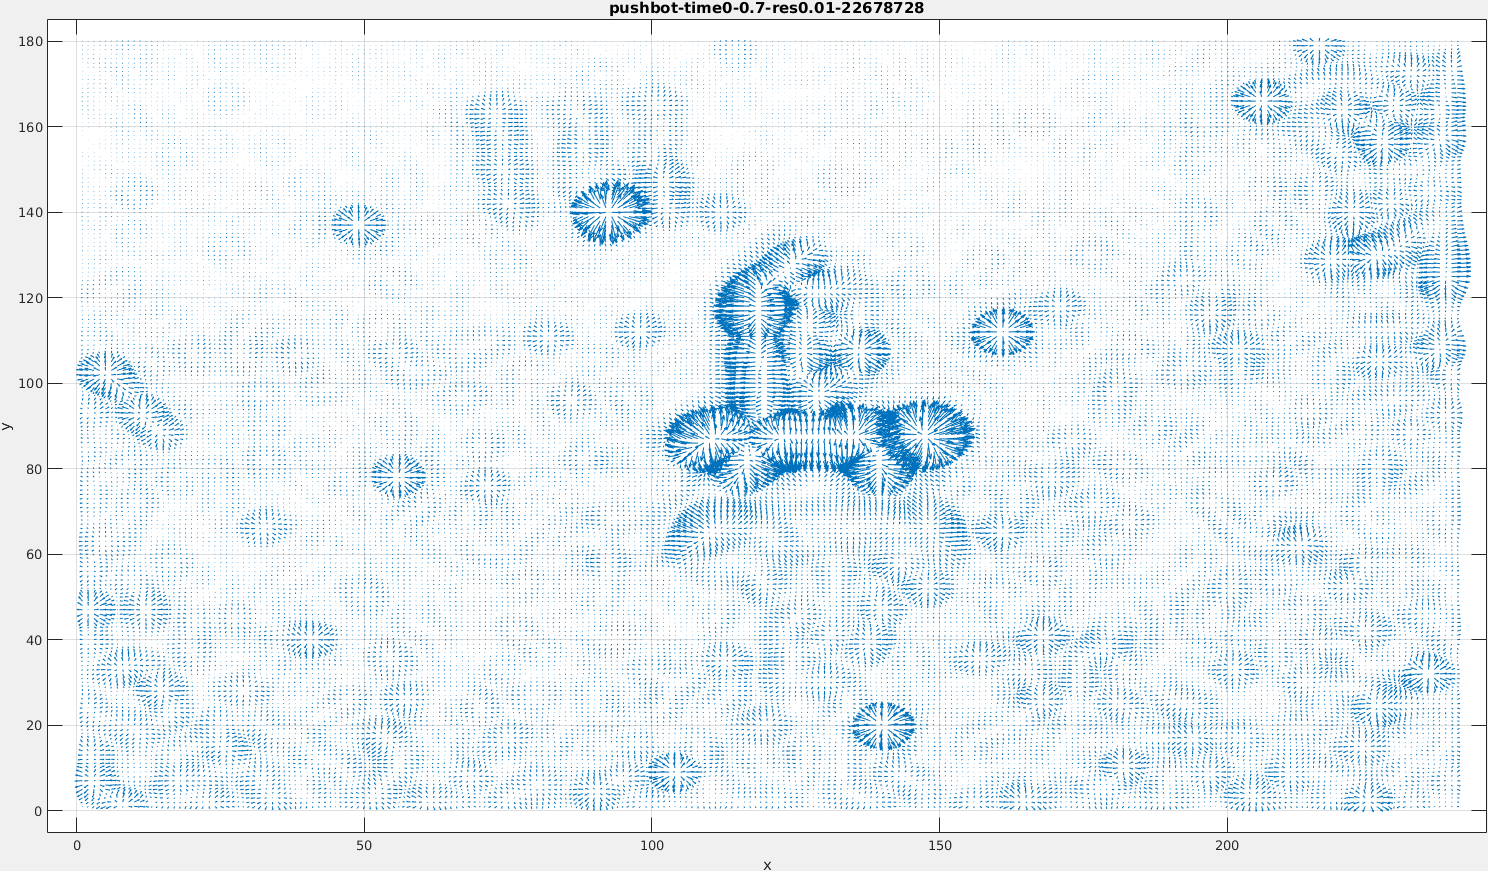
\includegraphics[height=.6\linewidth]{figs/pushbot/pushbot-1.png}
  \caption{}
\end{subfigure}
\begin{subfigure}{.45\textwidth}
  \centering
  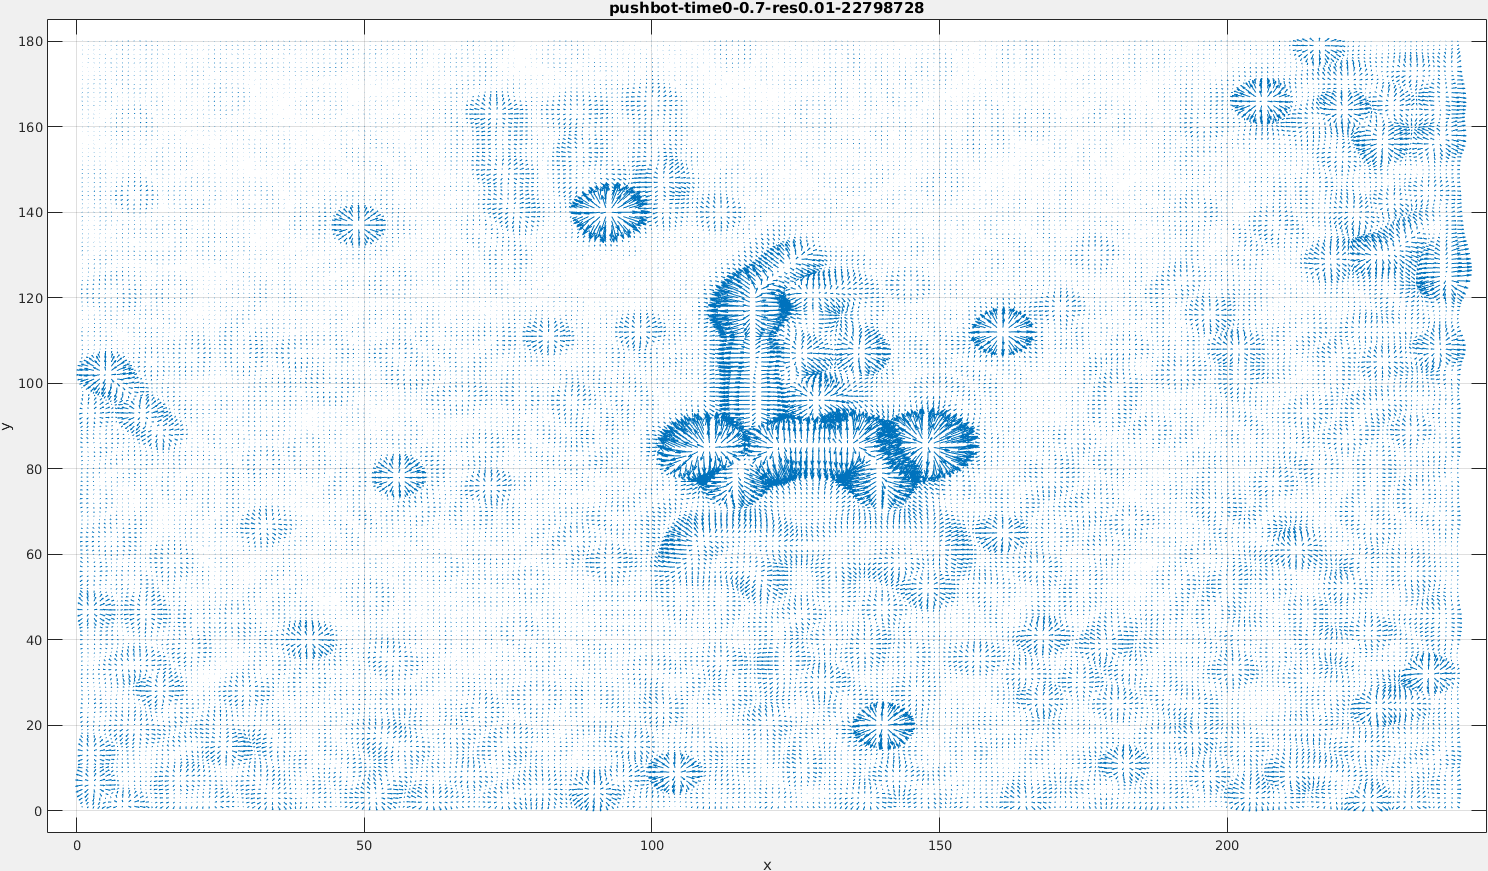
\includegraphics[height=.6\linewidth]{figs/pushbot/pushbot-2.png}
  \caption{}
\end{subfigure}
\begin{subfigure}{.45\textwidth}
  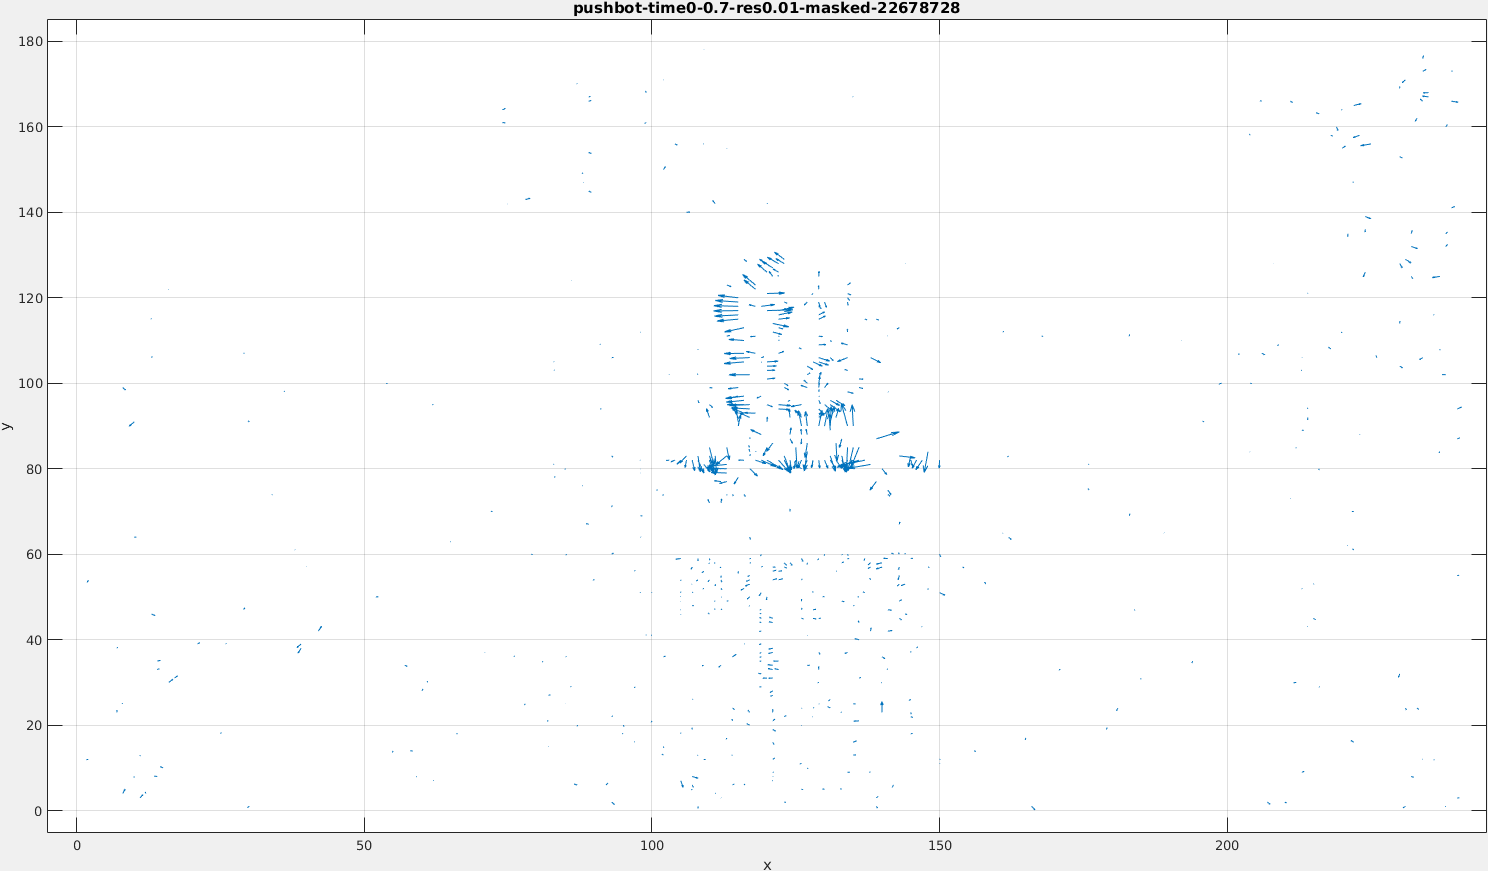
\includegraphics[height=.6\linewidth]{figs/pushbot/pushbot-masked-1.png}
  \caption{}
\end{subfigure}
\begin{subfigure}{.45\textwidth}
  \centering
  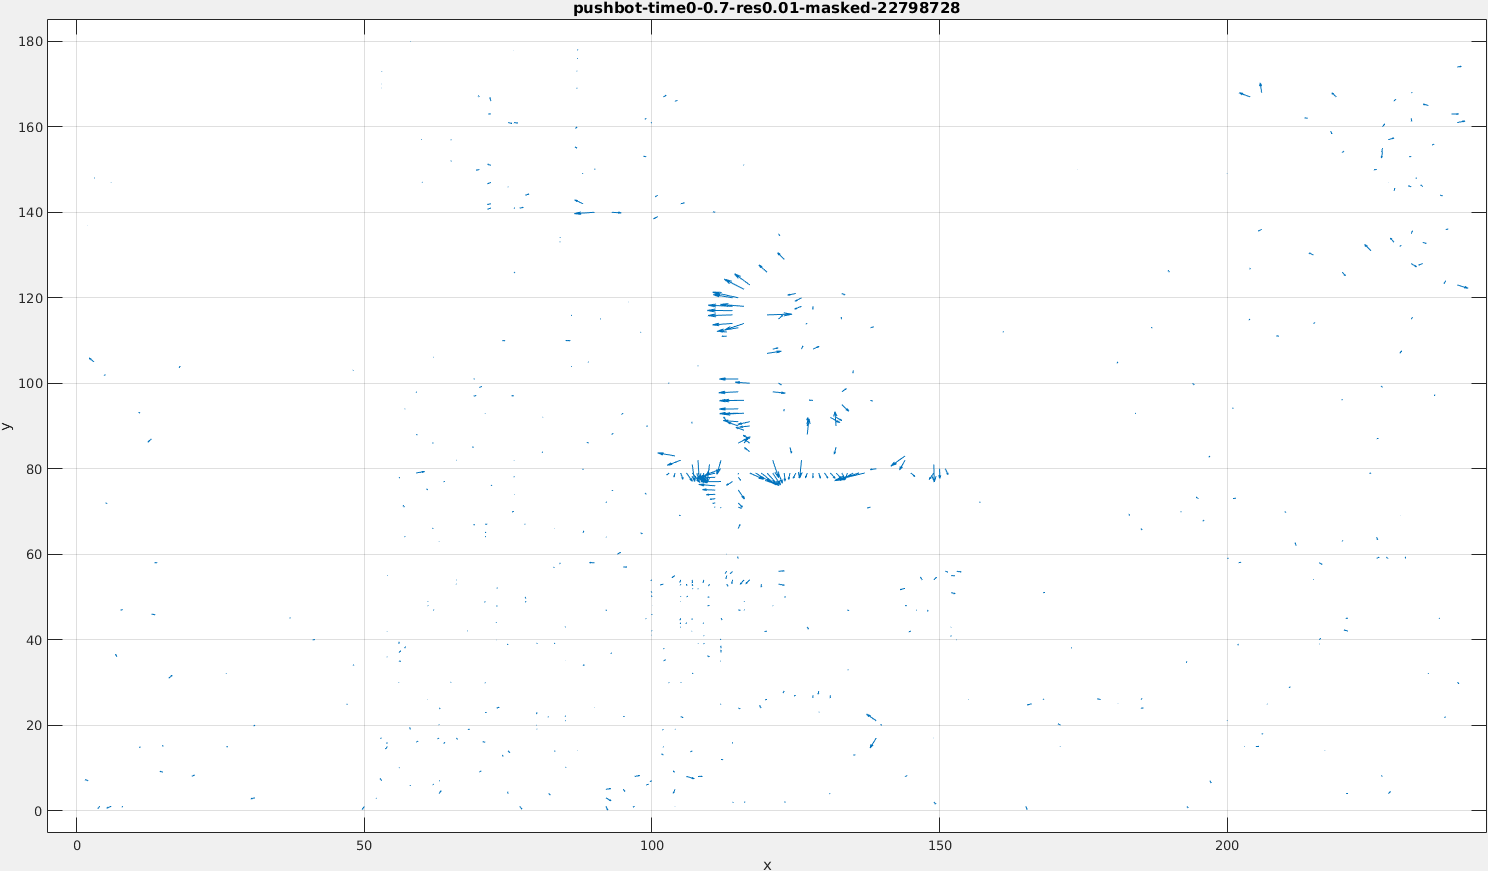
\includegraphics[height=.6\linewidth]{figs/pushbot/pushbot-masked-2.png}
  \caption{}
\end{subfigure}
\begin{subfigure}{.45\textwidth}
  \centering
  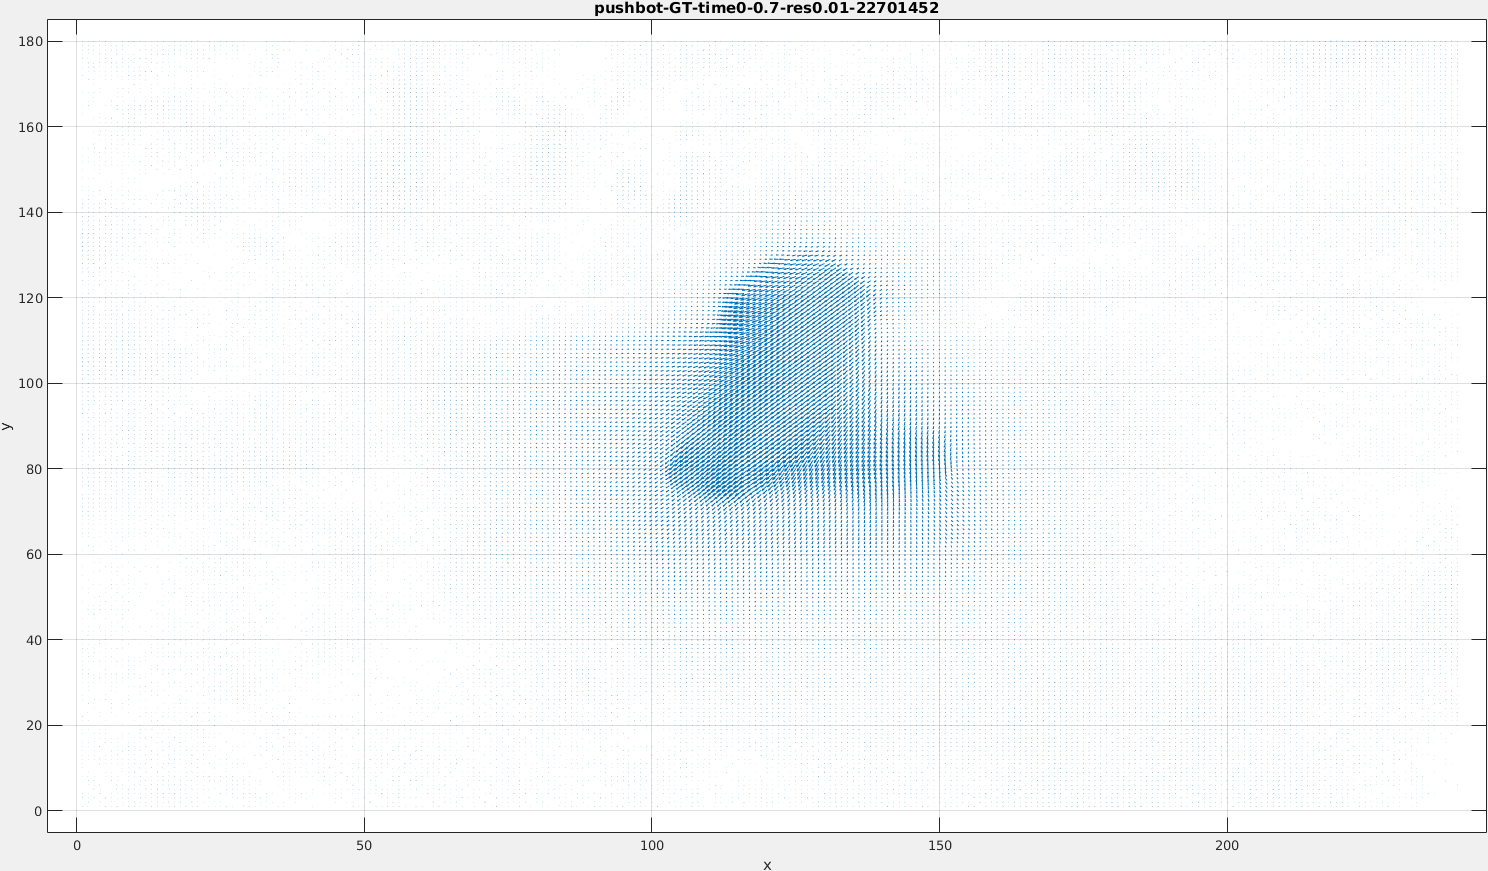
\includegraphics[height=.6\linewidth]{figs/pushbot/pushbot-GT-1.png}
  \caption{}
\end{subfigure}
\begin{subfigure}{.45\textwidth}
  \centering
  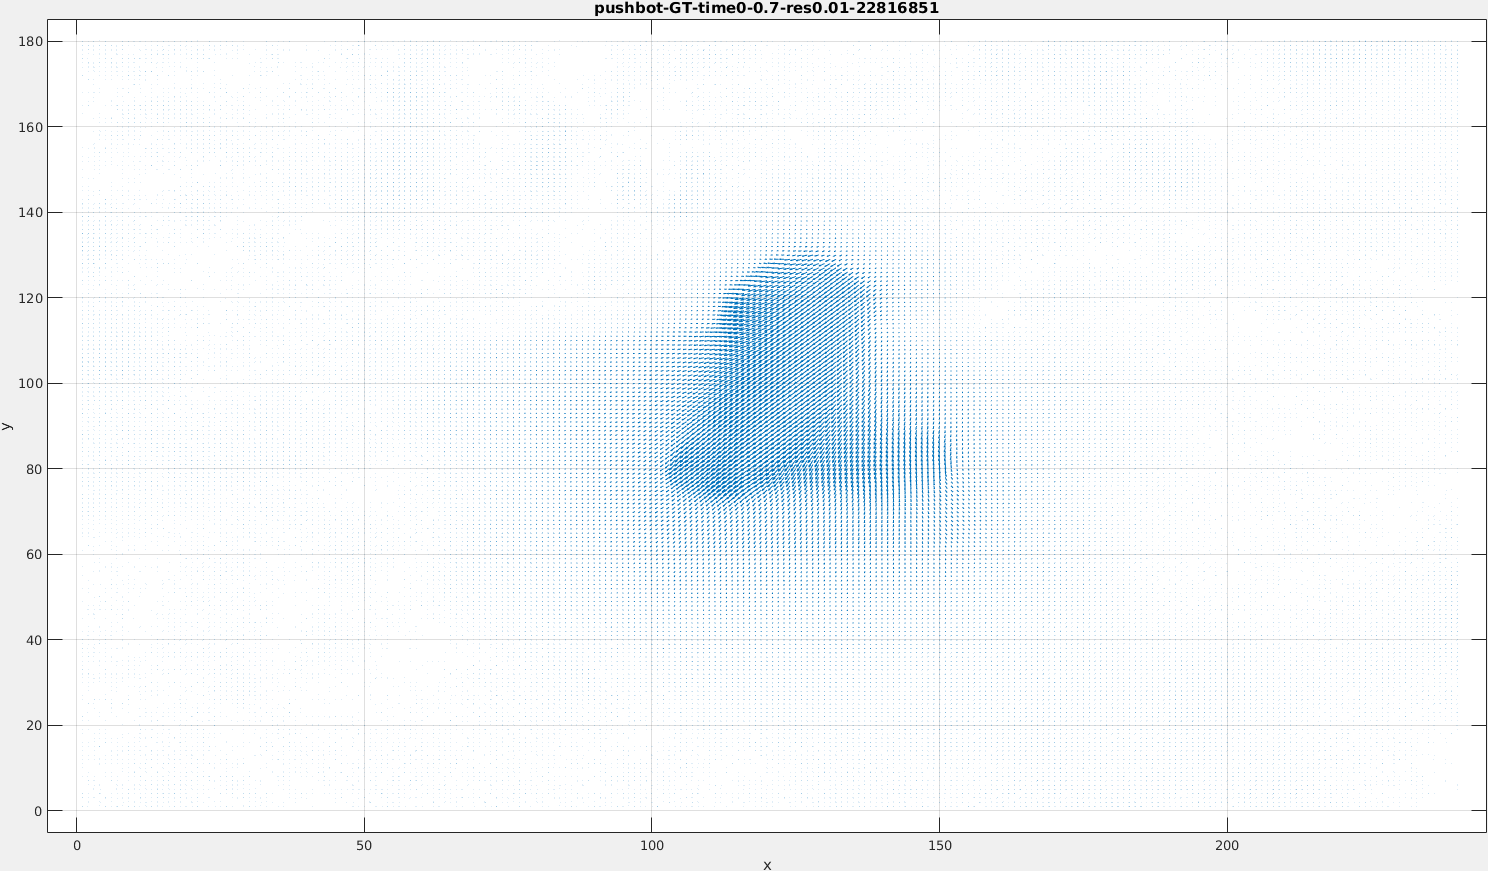
\includegraphics[height=.6\linewidth]{figs/pushbot/pushbot-GT-2.png}
  \caption{}
\end{subfigure}
\begin{subfigure}{.45\textwidth}
  \centering
  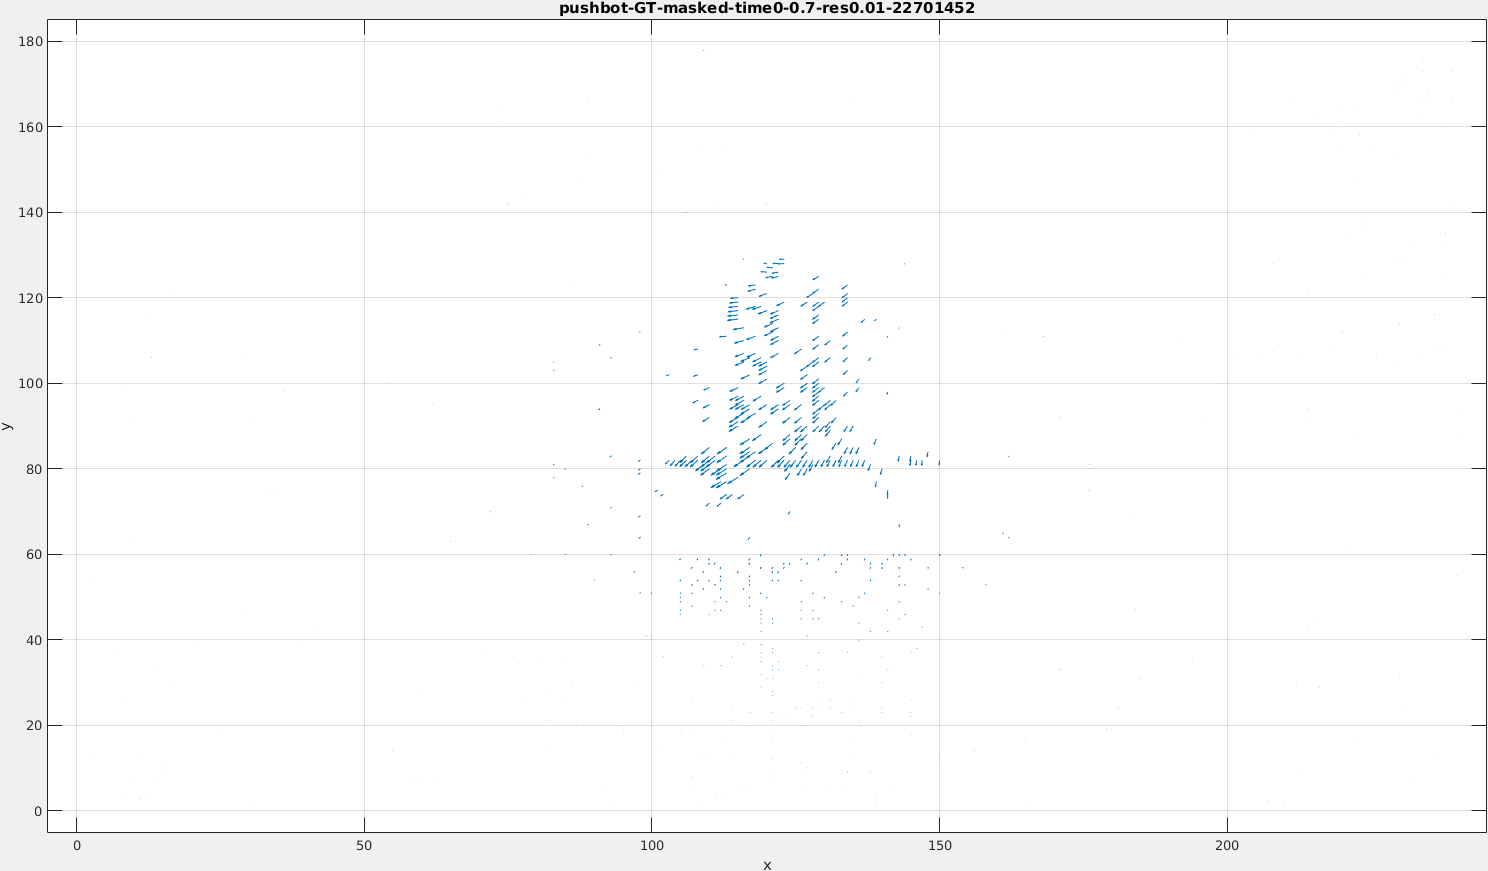
\includegraphics[height=.6\linewidth]{figs/pushbot/pushbot-GT-masked-1.png}
  \caption{}
\end{subfigure}
\begin{subfigure}{.45\textwidth}
  \centering
  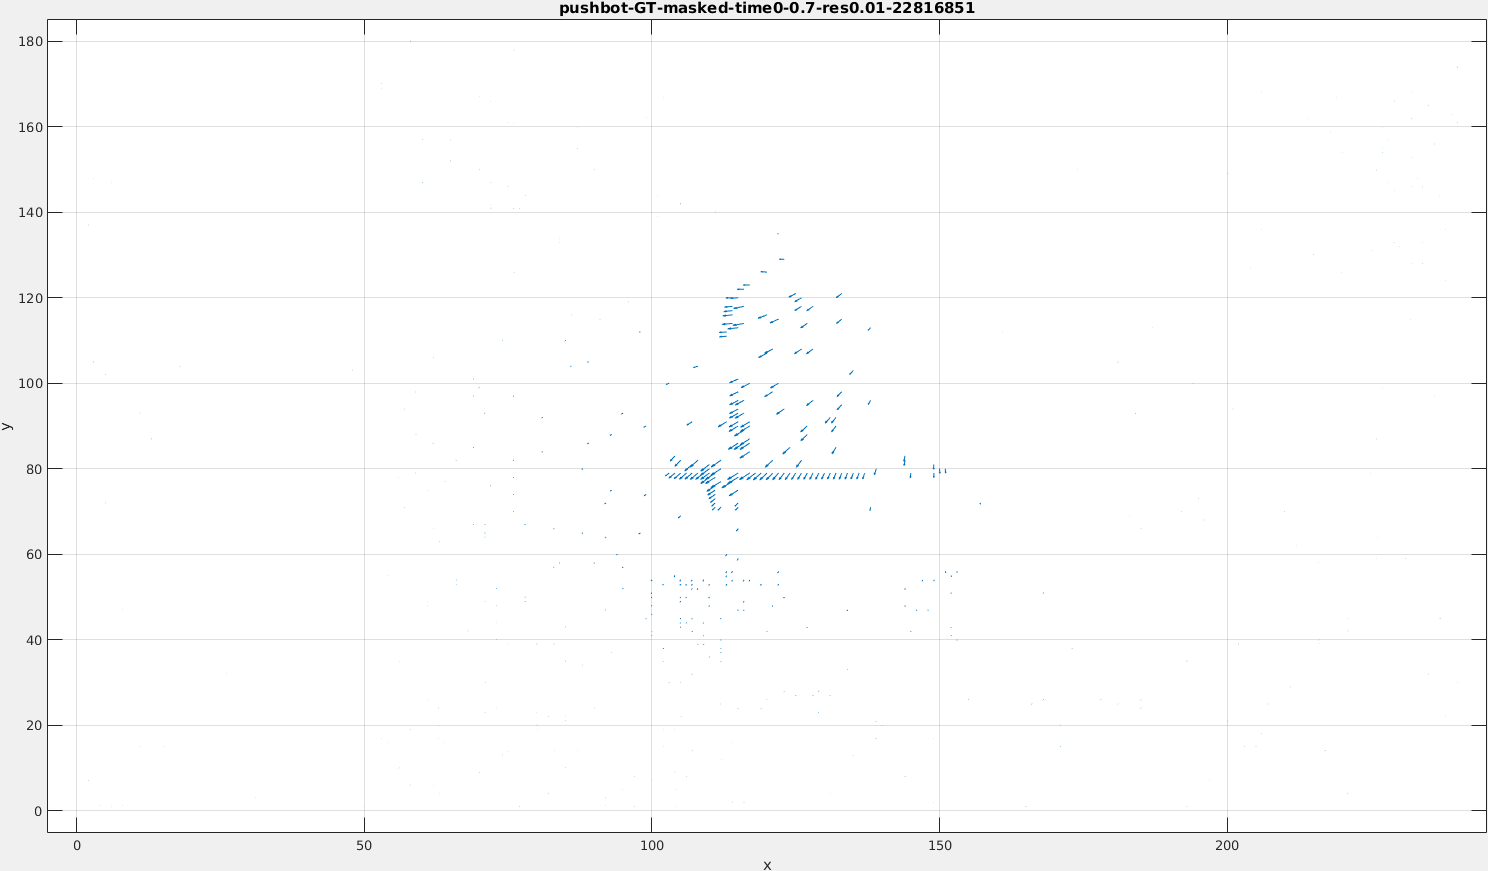
\includegraphics[height=.6\linewidth]{figs/pushbot/pushbot-GT-masked-2.png}
  \caption{}
\end{subfigure}
\caption[Second scene: Robot approaching the DVS sensor.]{Second scene: A small robot is approaching the DVS sensor. Figures (a) and (b) show the computed optical flow for the scene at two time steps. The masked flow fields are shown in Figures (c) and (d).
The corresponding ground truth is shown in Figures (e) and (f). Applying the same mask leads to Figures (g) and (h).
In the ground truth it can be observed that flow is directed to the bottom left of the frame (g)(h). 
In the computed flow, a horizontal edge at the bottom and a vertical edge at the left of the robot are clearly visible (c)(d).
The flow pointing from these edges indicates the direction of movement. 
It is most likely not pointing to the bottom left because of the missing normalization.}
\label{fig:app_pushbot-snapshots}
\end{figure}


\begin{figure}[tb]
\centering
\begin{subfigure}{.45\textwidth}
  \centering
  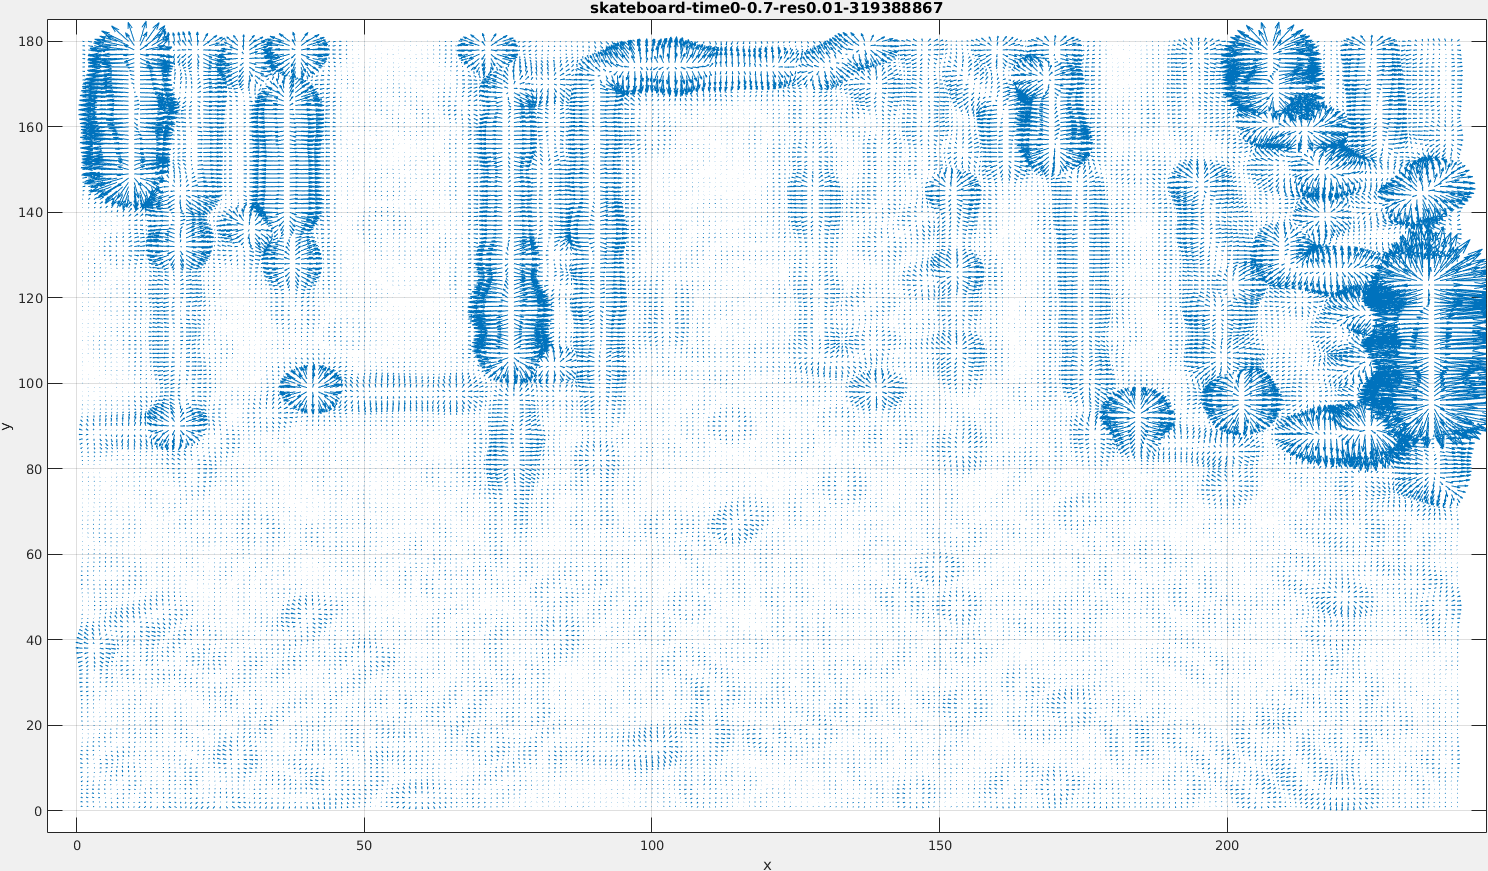
\includegraphics[height=.6\linewidth]{figs/skateboard/skateboard-1.png}
  \caption{}
%  \label{fig:skateboard-snapshots1}
\end{subfigure}
\begin{subfigure}{.45\textwidth}
  \centering
  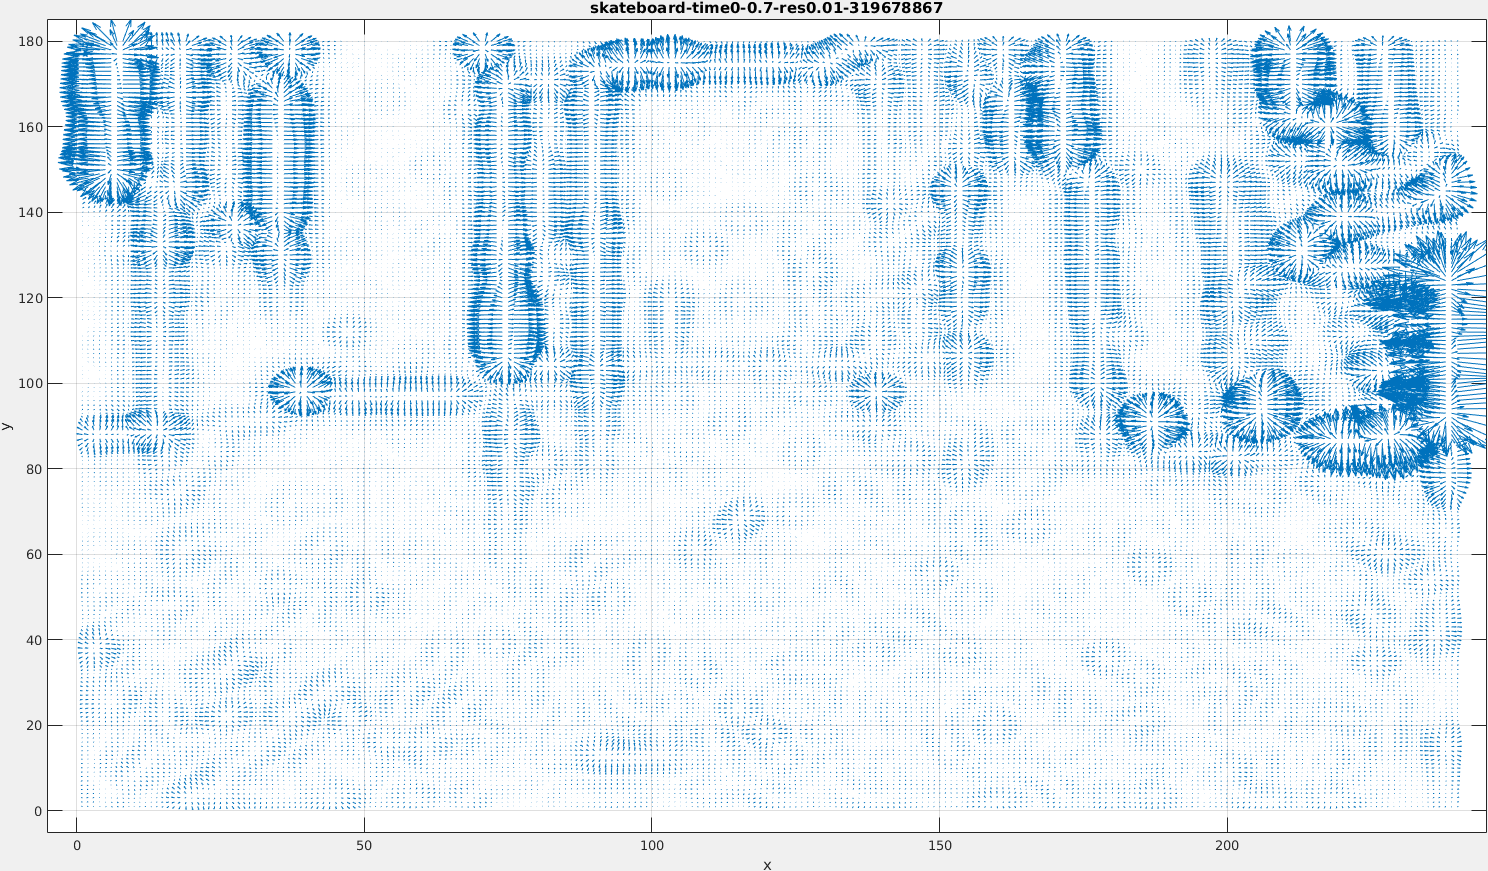
\includegraphics[height=.6\linewidth]{figs/skateboard/skateboard-2.png}
  \caption{}
%  \label{fig:skateboard-snapshots2}
\end{subfigure}
\begin{subfigure}{.45\textwidth}
  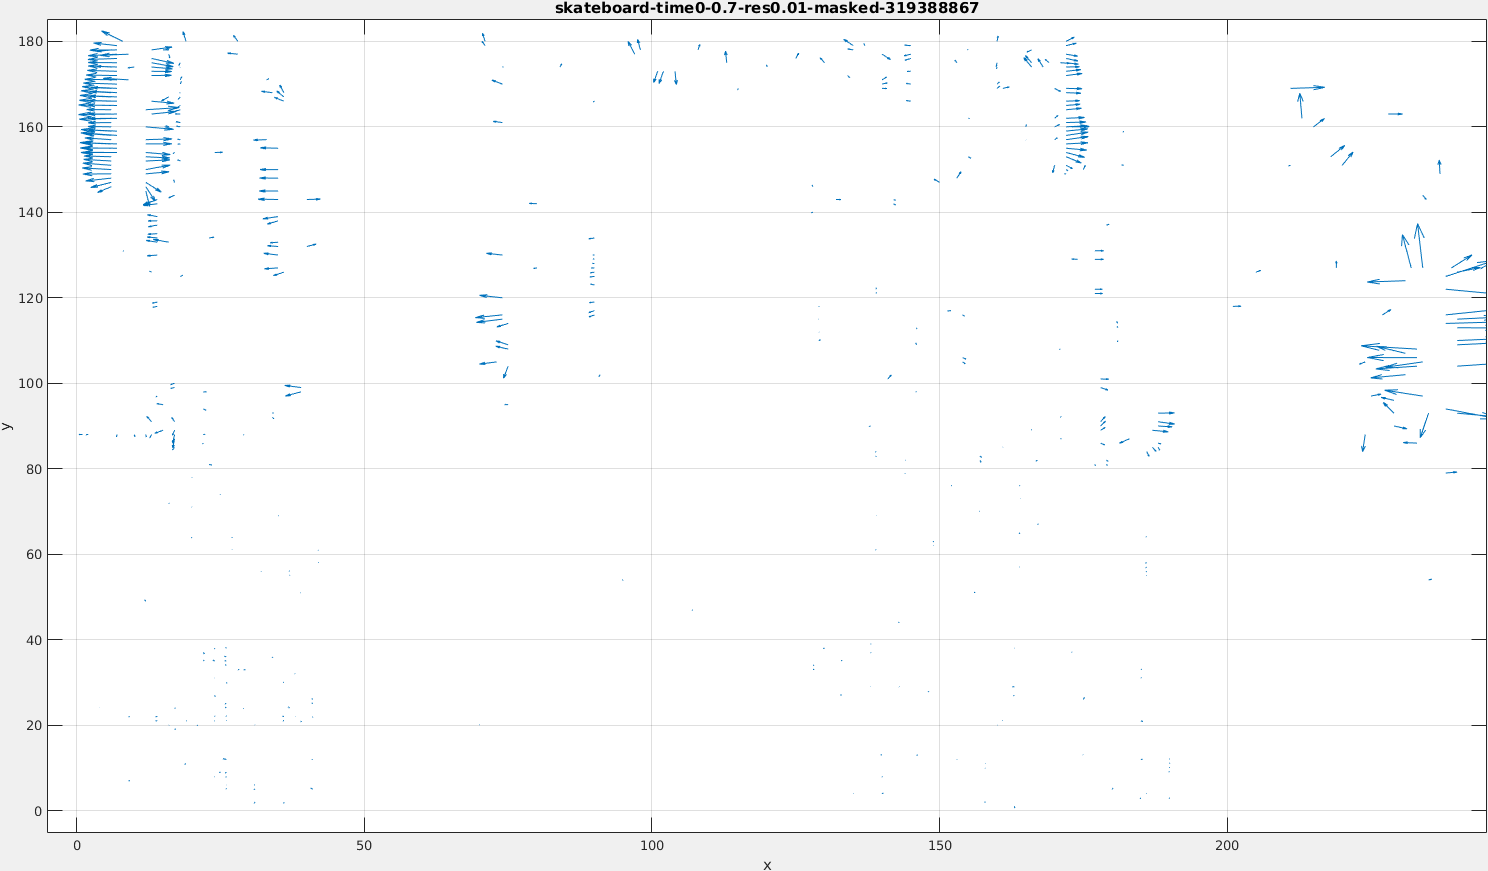
\includegraphics[height=.6\linewidth]{figs/skateboard/skateboard-masked-1.png}
  \caption{}
\end{subfigure}
\begin{subfigure}{.45\textwidth}
  \centering
  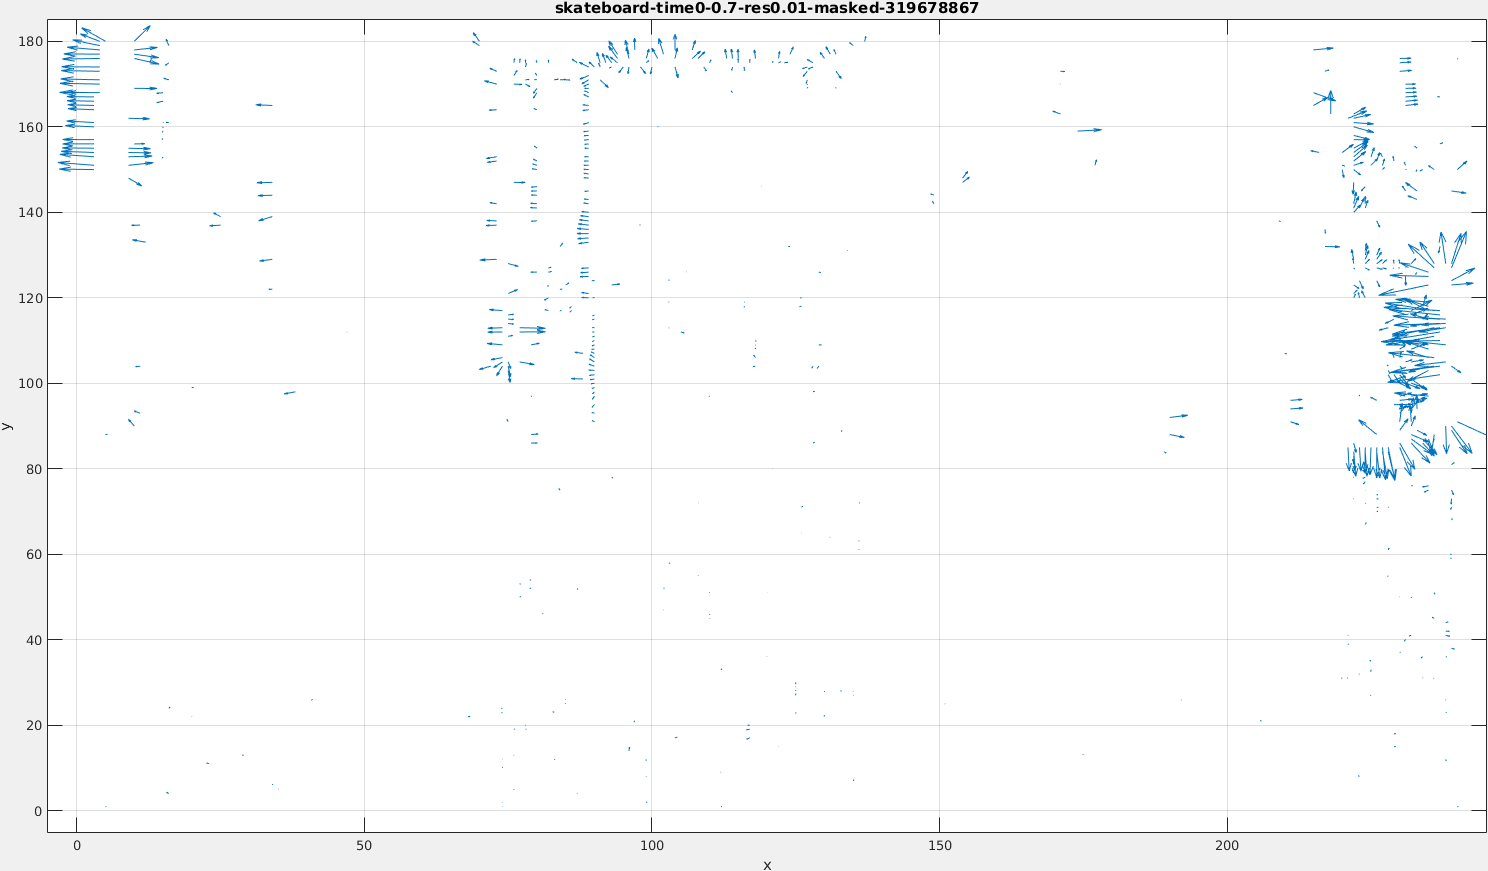
\includegraphics[height=.6\linewidth]{figs/skateboard/skateboard-masked-2.png}
  \caption{}
\end{subfigure}
\begin{subfigure}{.45\textwidth}
  \centering
  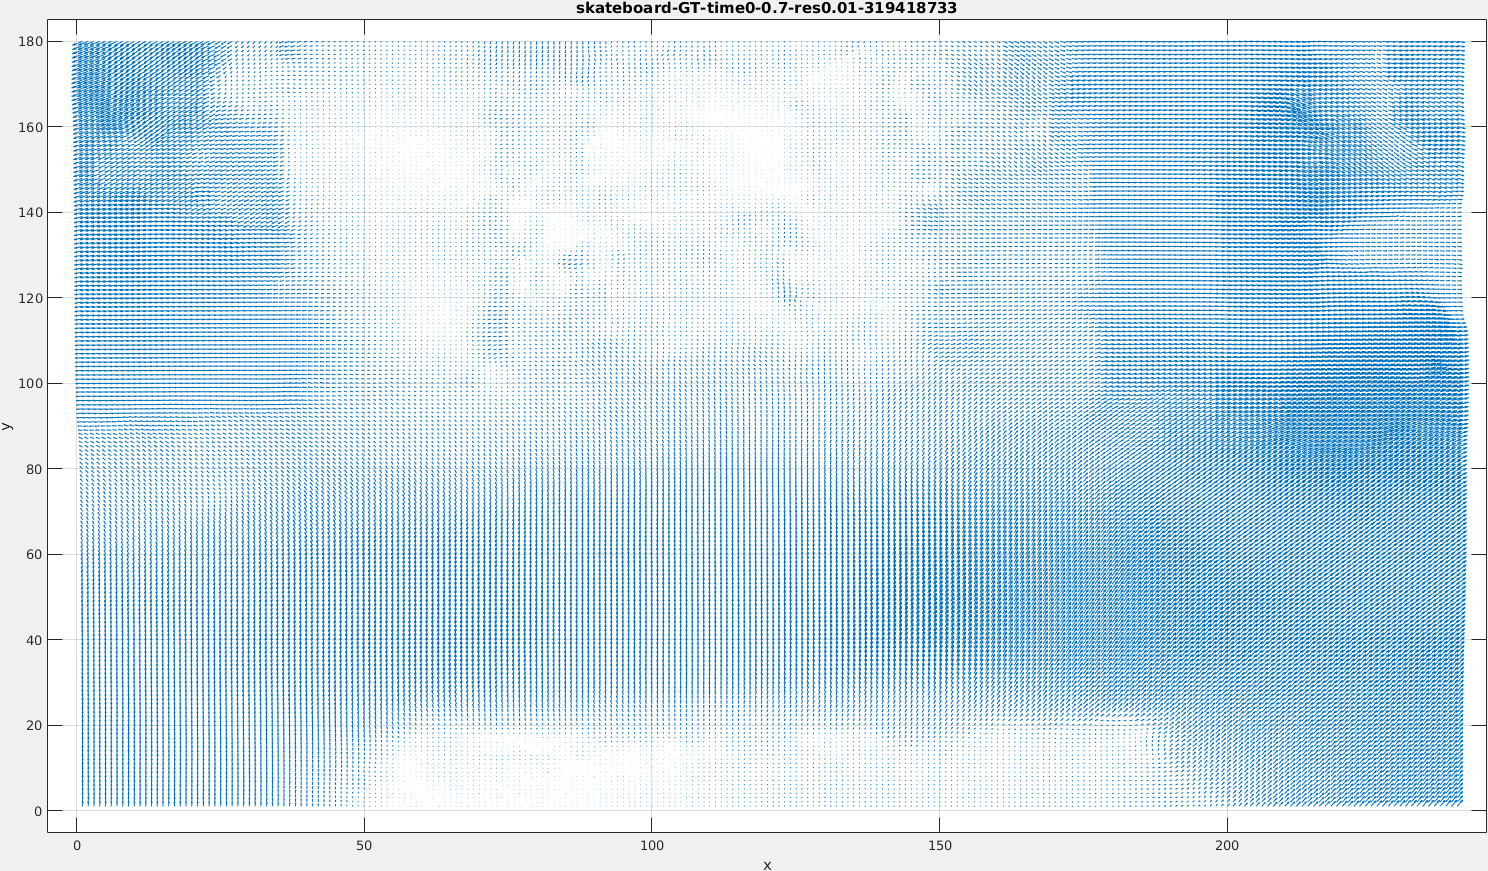
\includegraphics[height=.6\linewidth]{figs/skateboard/skateboard-GT-1.png}
  \caption{}
\end{subfigure}
\begin{subfigure}{.45\textwidth}
  \centering
  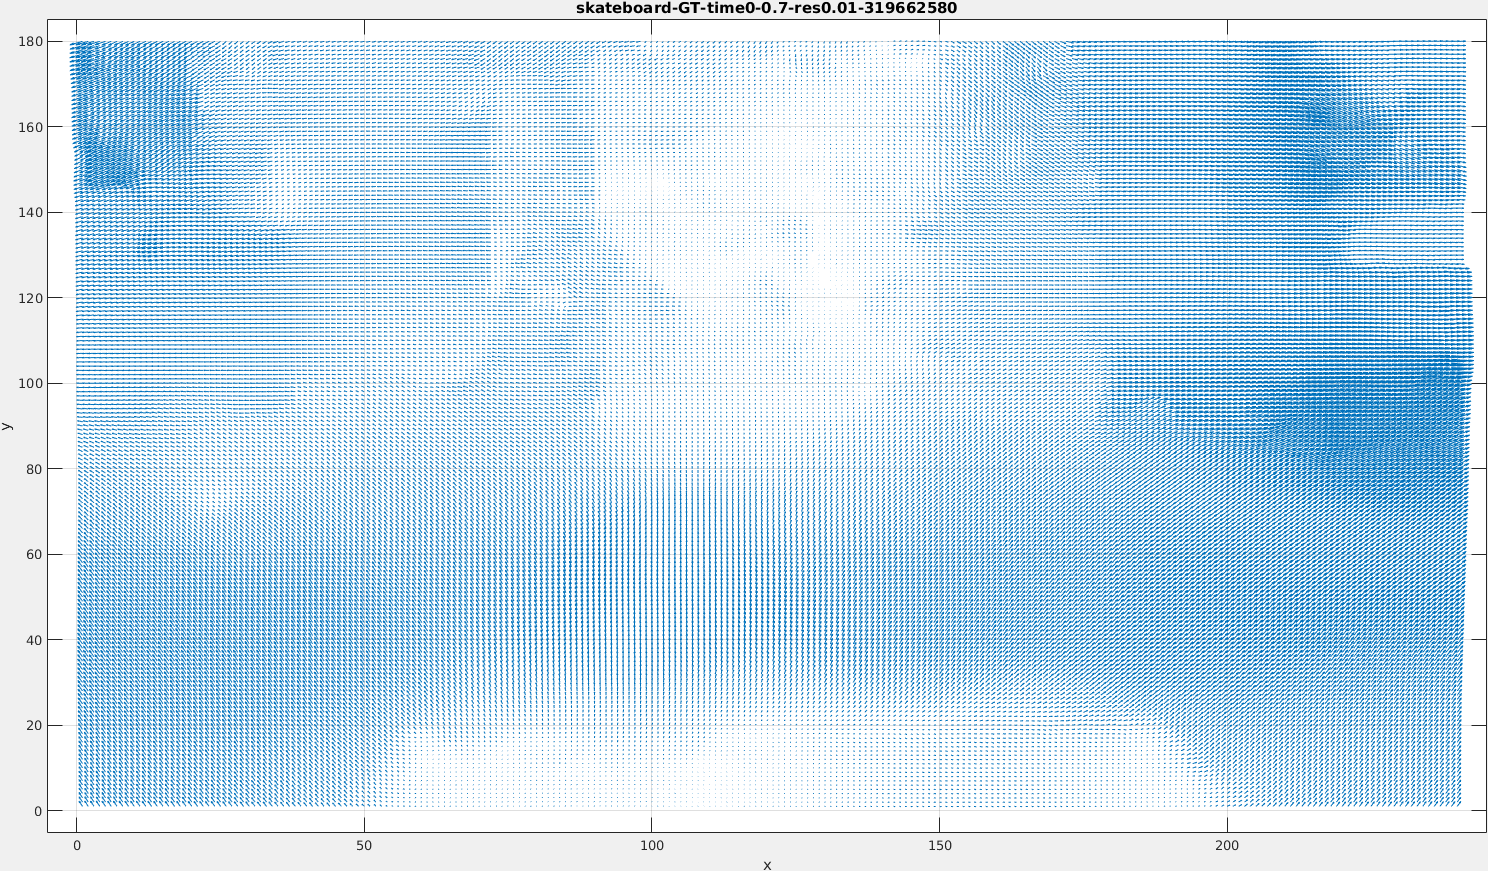
\includegraphics[height=.6\linewidth]{figs/skateboard/skateboard-GT-2.png}
  \caption{}
\end{subfigure}
\begin{subfigure}{.45\textwidth}
  \centering
  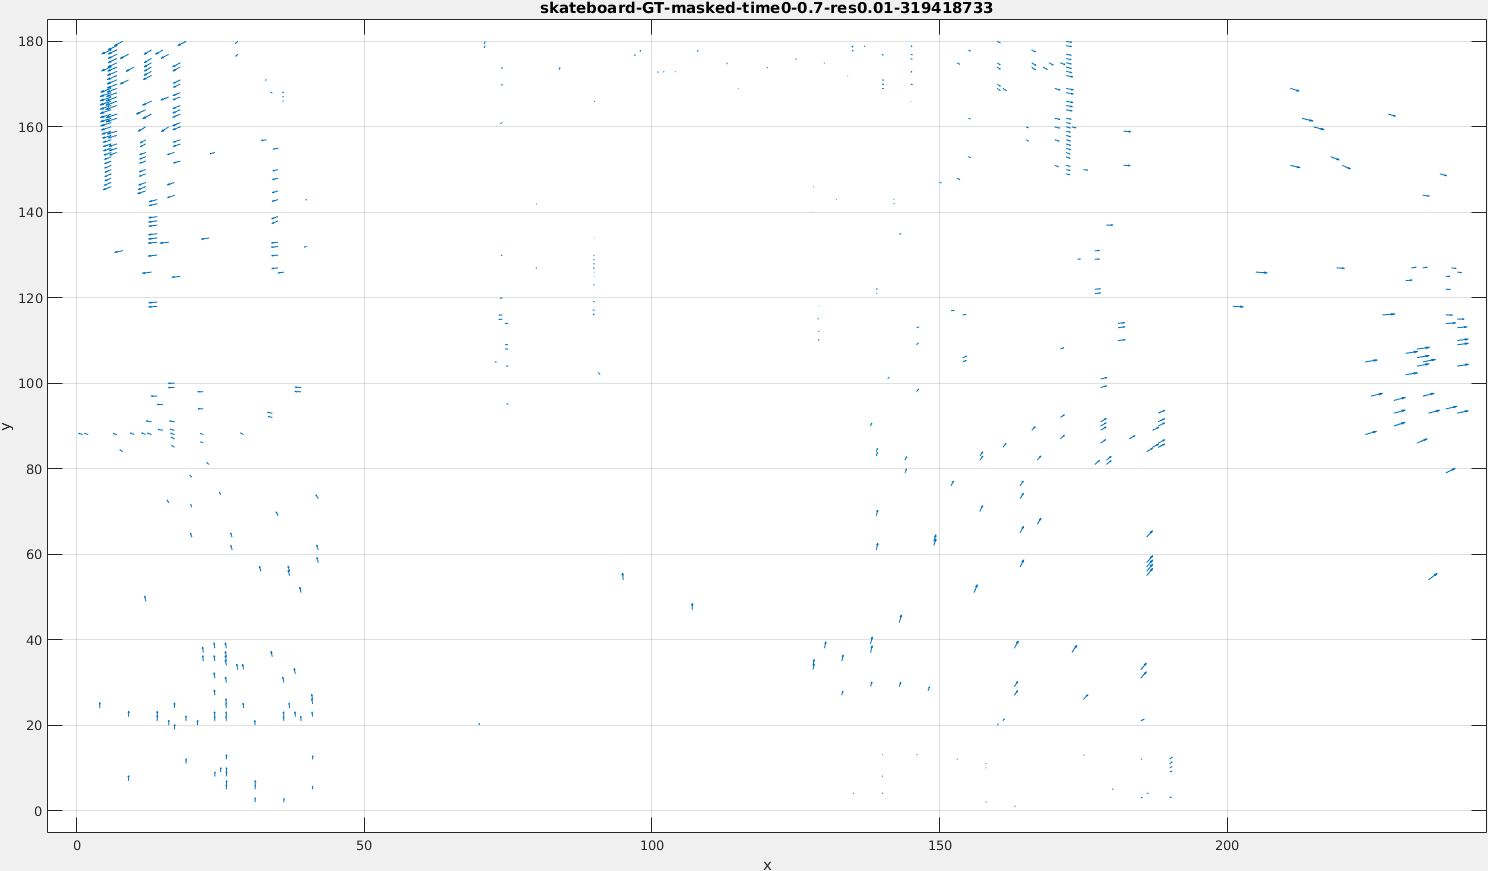
\includegraphics[height=.6\linewidth]{figs/skateboard/skateboard-GT-masked-1.png}
  \caption{}
\end{subfigure}
\begin{subfigure}{.45\textwidth}
  \centering
  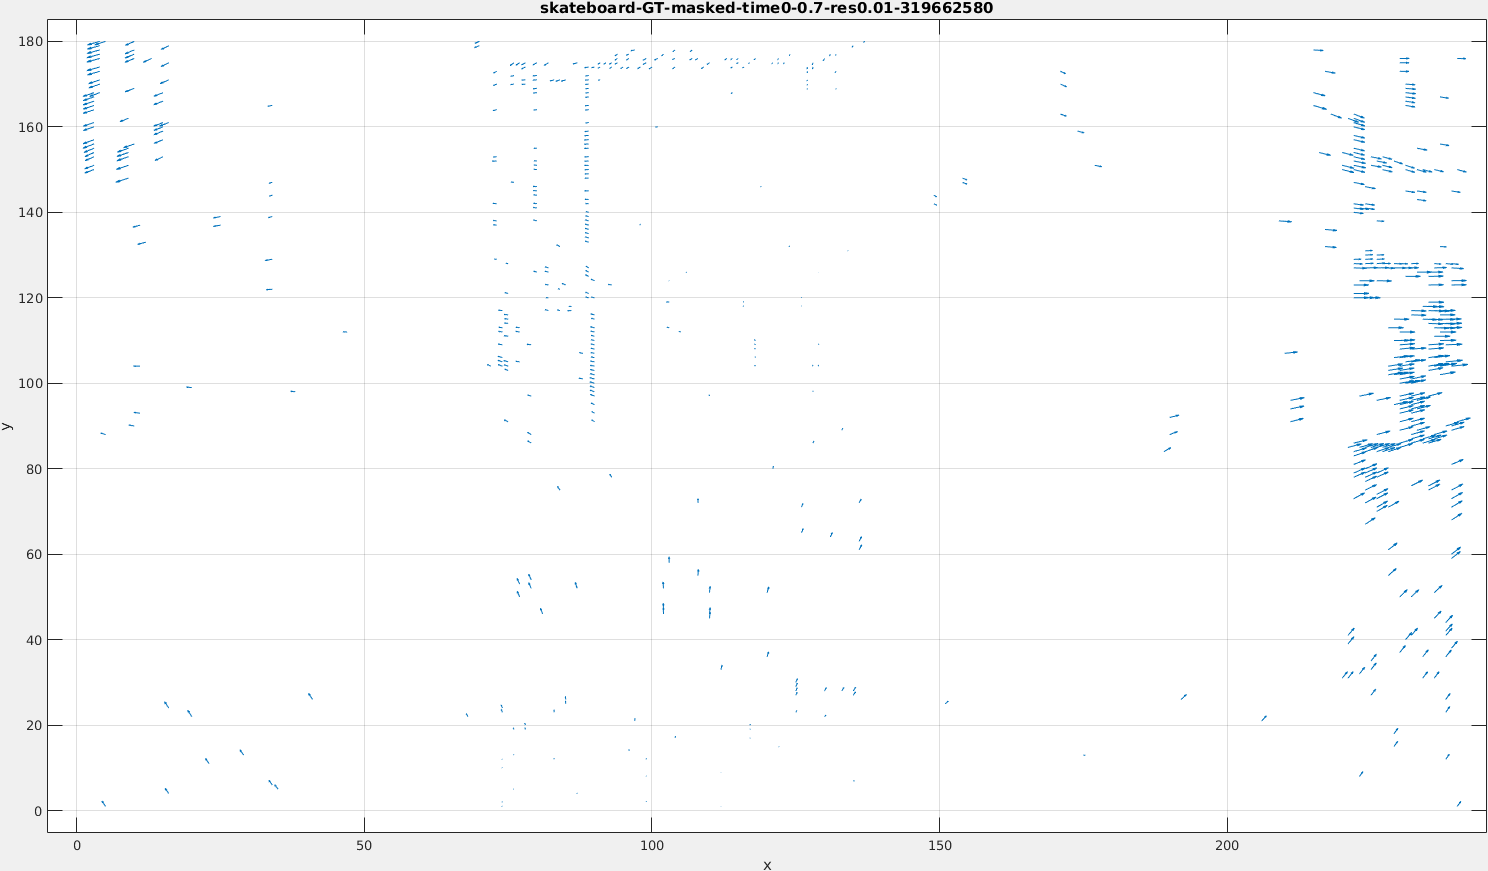
\includegraphics[height=.6\linewidth]{figs/skateboard/skateboard-GT-masked-2.png}
  \caption{}
\end{subfigure}
\caption[Third scene: Moving DVS sensor observing interior of a room.]{Third scene: Moving DVS sensor observing interior of a room. 
Figures (a) and (b) show the computed optical flow for the scene at two time steps. The masked flow fields are shown in Figures (c) and (d).
The corresponding ground truth is shown in Figures (e) and (f). 
Applying the same mask leads to Figures (g) and (h).

The computed flow clearly detects edges and dominant structures in the room (a)(b).
Trough masking, the visual similarities between the results (Figures (c) and (d)) and the ground truth ((g) and (h)) at the event locations become visible.
}
\label{fig:app_skateboard-snapshots}
\end{figure}

\begin{figure}[tb]
\centering
\begin{subfigure}{.45\textwidth}
  \centering
  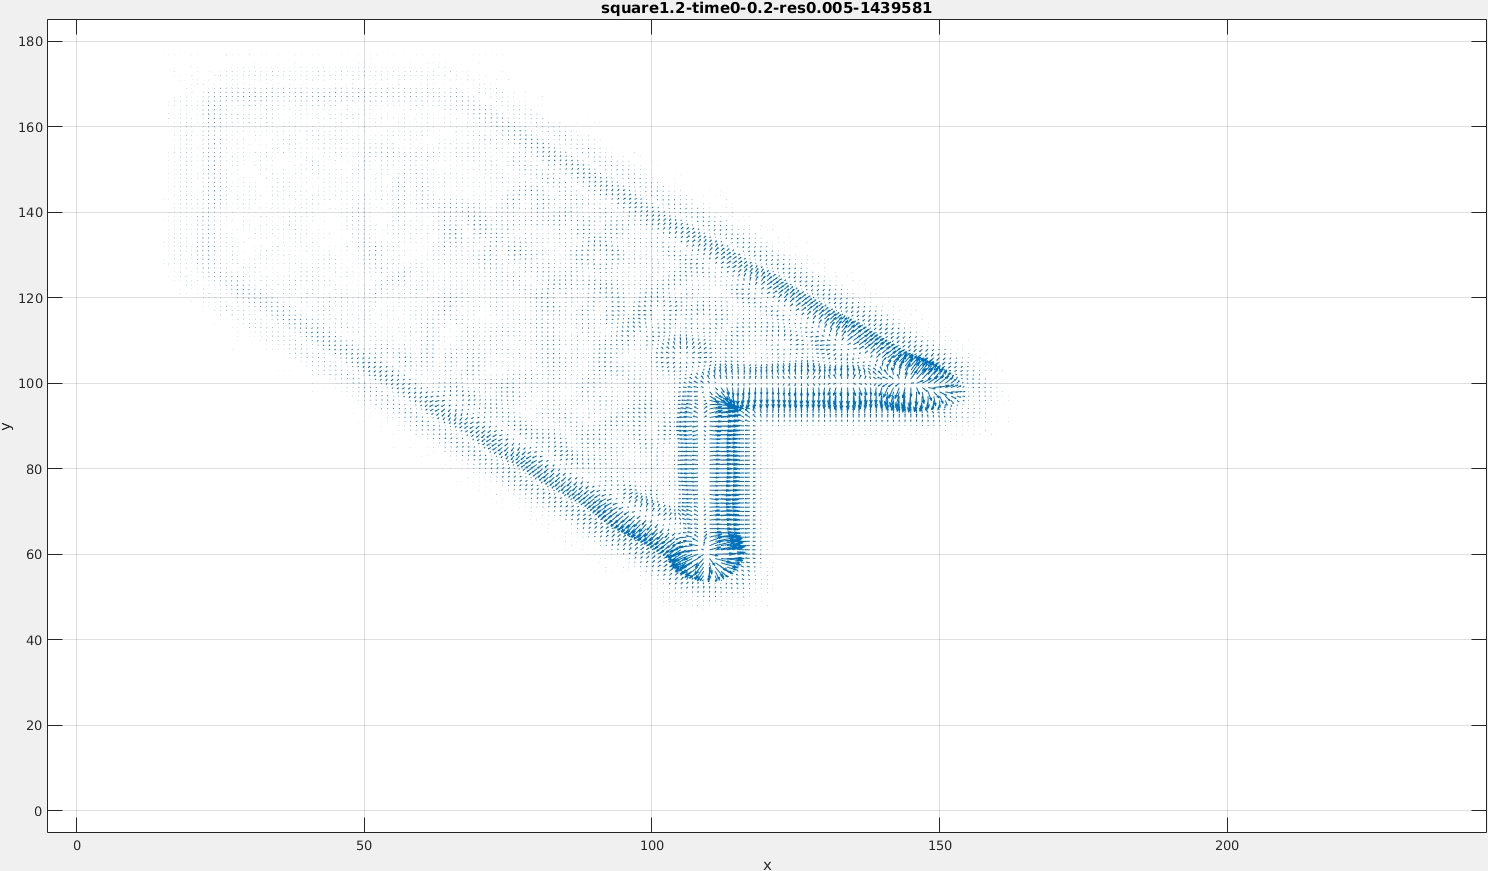
\includegraphics[height=.6\linewidth]{figs/square12/square12-1.png}
  \caption{}
\end{subfigure}
\begin{subfigure}{.45\textwidth}
  \centering
  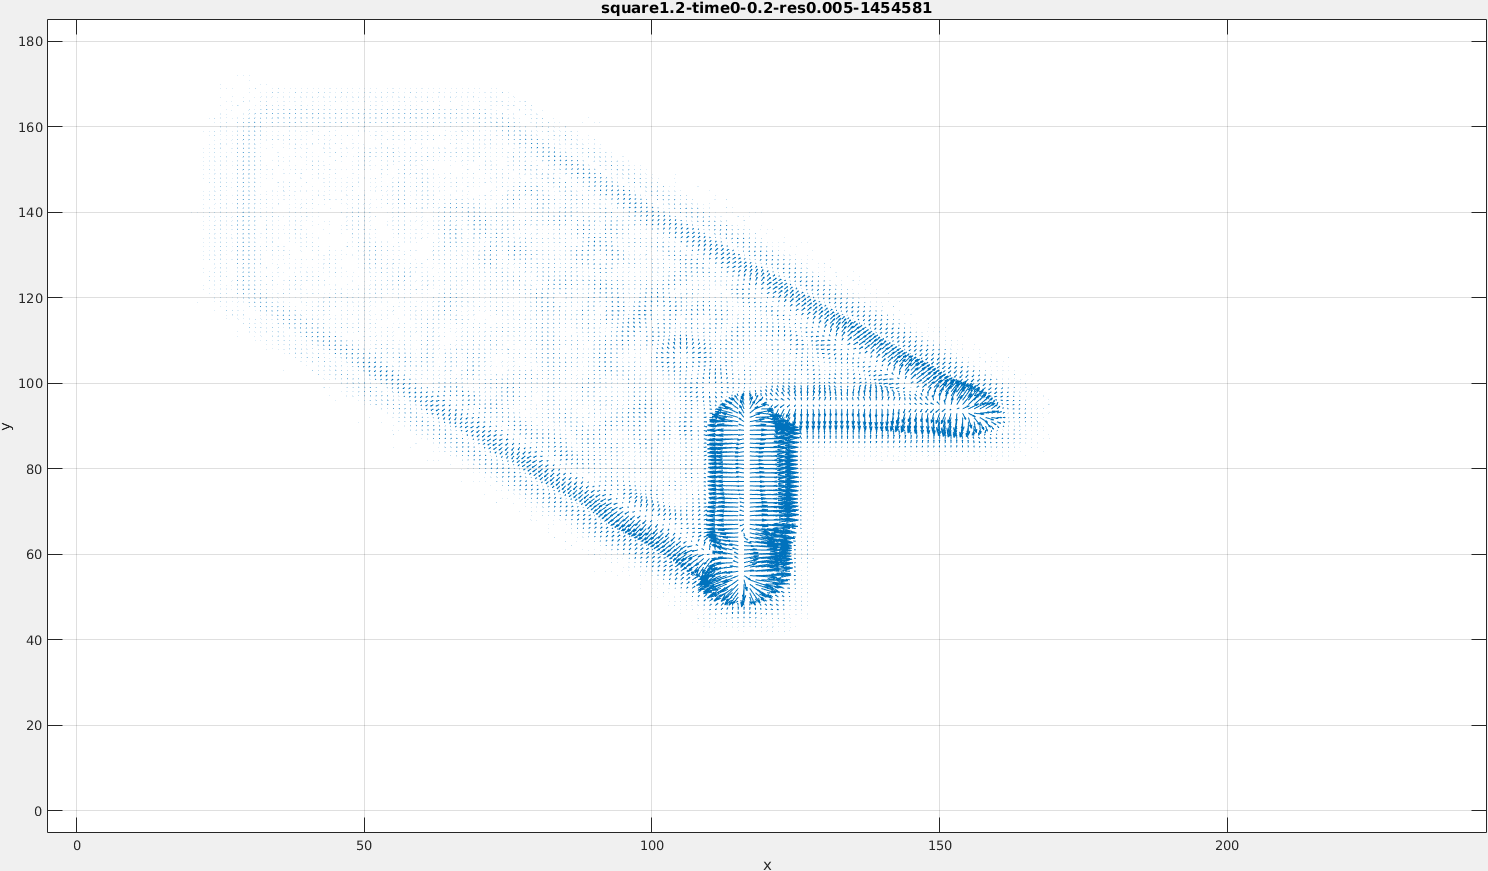
\includegraphics[height=.6\linewidth]{figs/square12/square12-2.png}
  \caption{}
\end{subfigure}
\begin{subfigure}{.45\textwidth}
  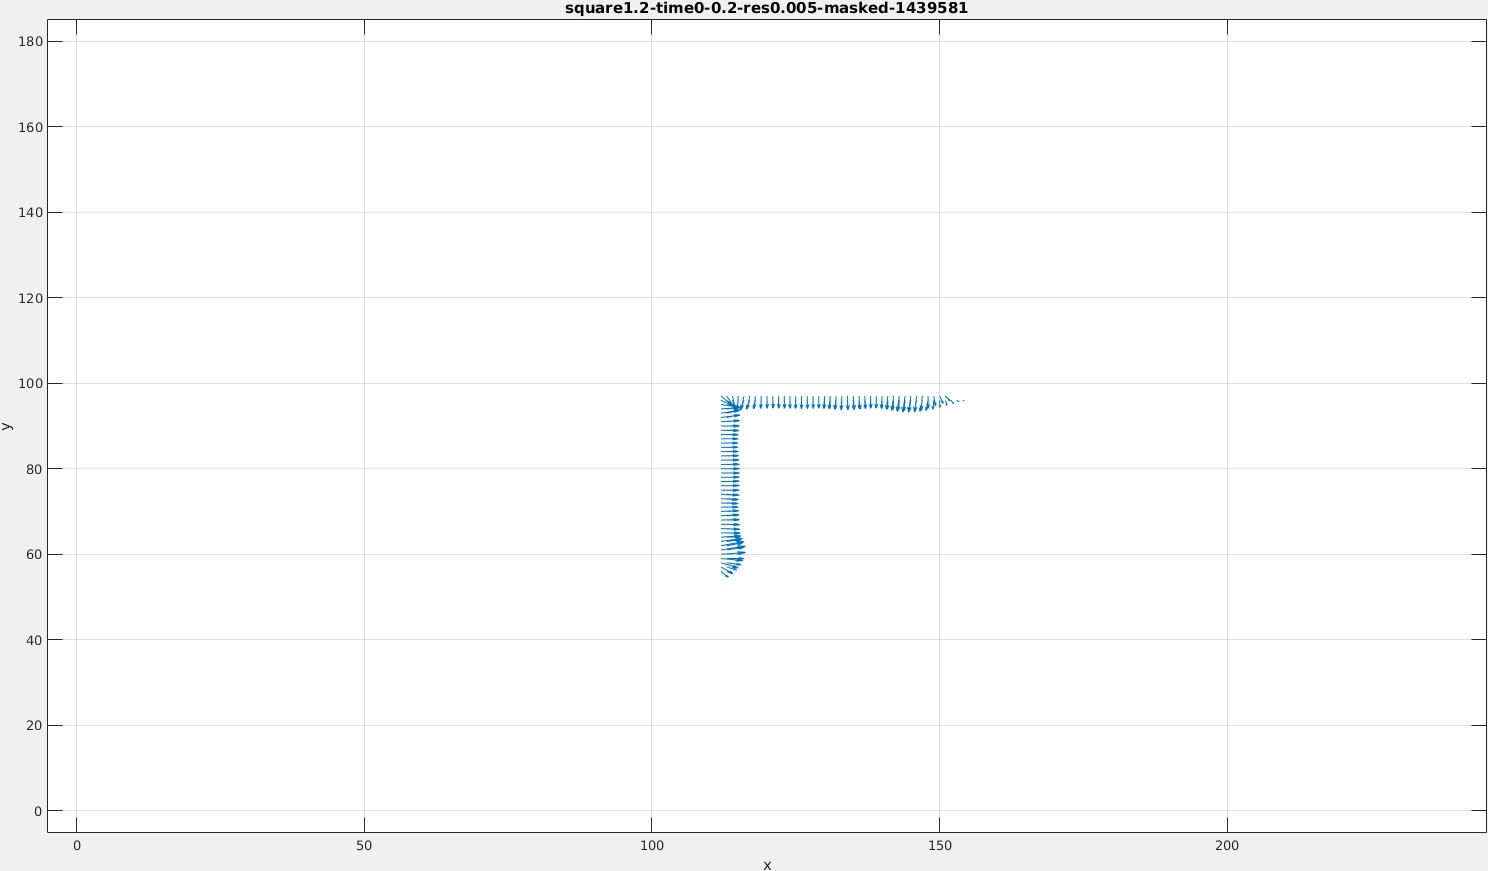
\includegraphics[height=.6\linewidth]{figs/square12/square12-masked-1.png}
  \caption{}
\end{subfigure}
\begin{subfigure}{.45\textwidth}
  \centering
  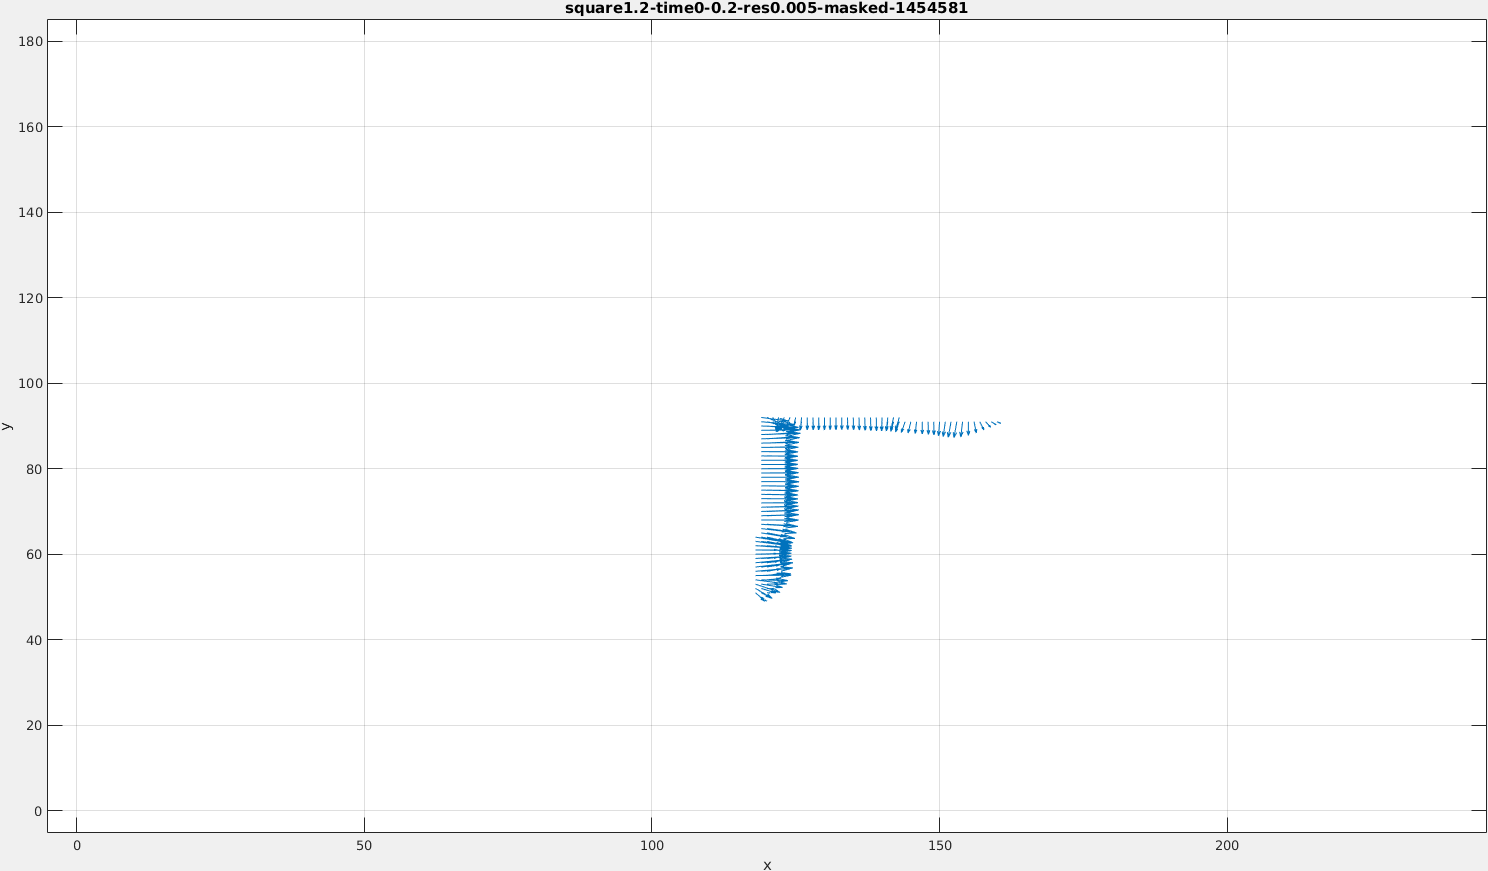
\includegraphics[height=.6\linewidth]{figs/square12/square12-masked-2.png}
  \caption{}
\end{subfigure}
\begin{subfigure}{.45\textwidth}
  \centering
  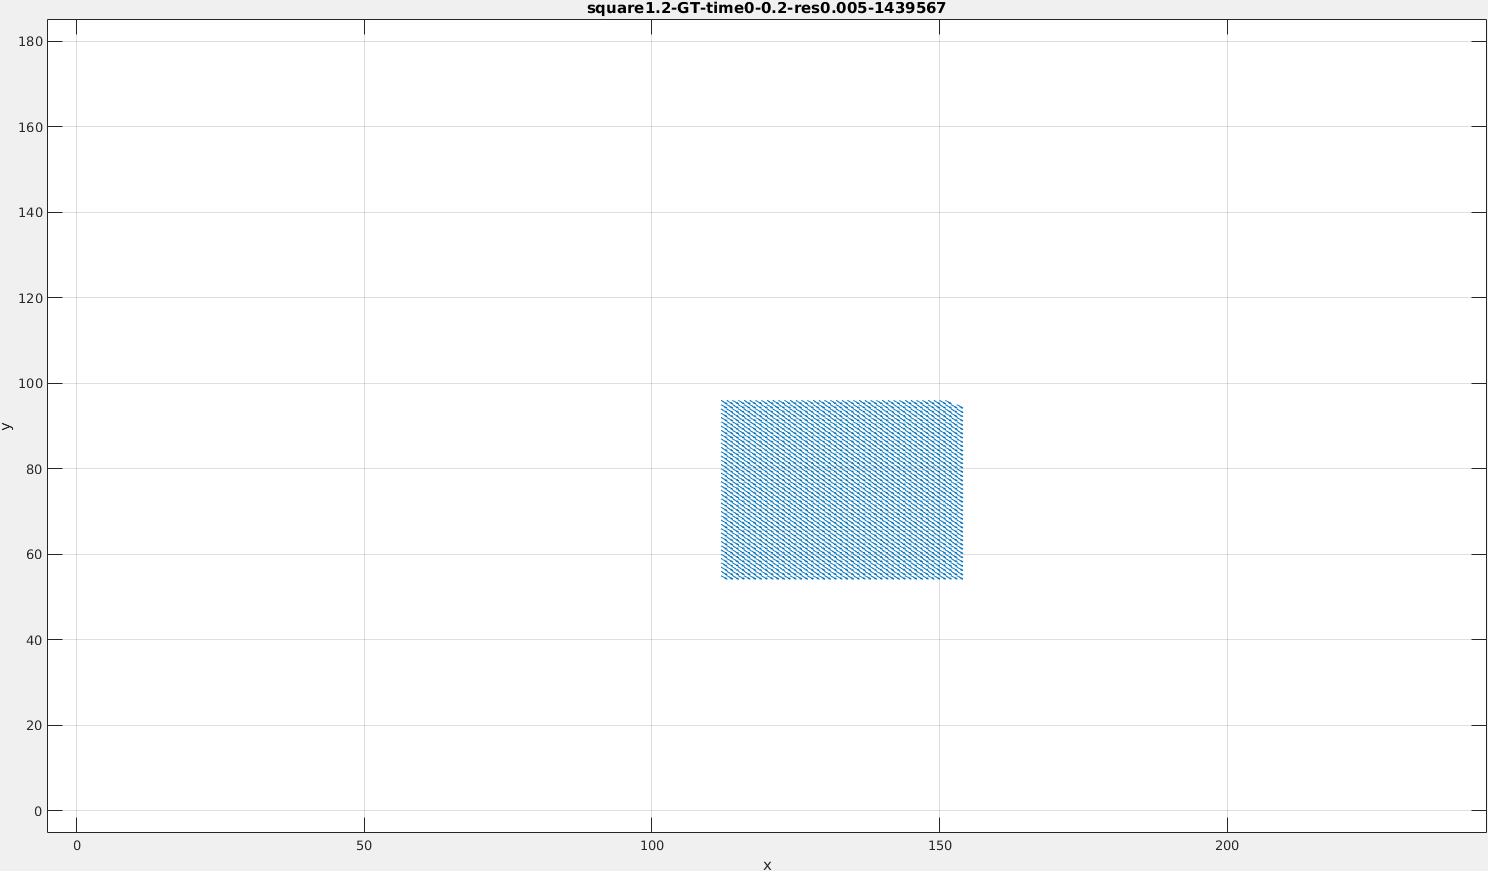
\includegraphics[height=.6\linewidth]{figs/square12/square12-GT-1.png}
  \caption{}
\end{subfigure}
\begin{subfigure}{.45\textwidth}
  \centering
  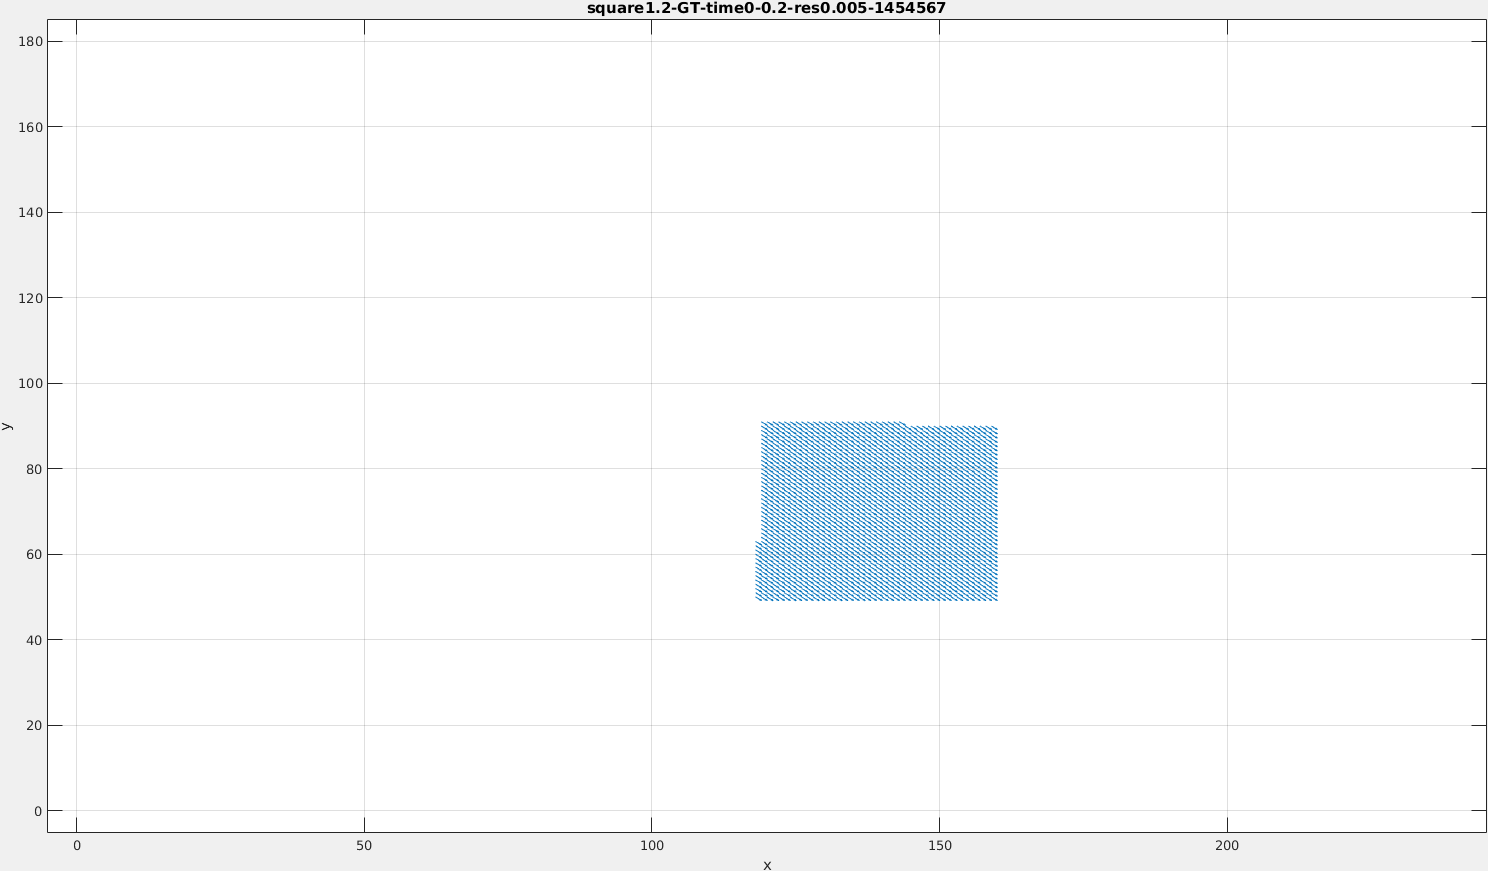
\includegraphics[height=.6\linewidth]{figs/square12/square12-GT-2.png}
  \caption{}
\end{subfigure}
\begin{subfigure}{.45\textwidth}
  \centering
  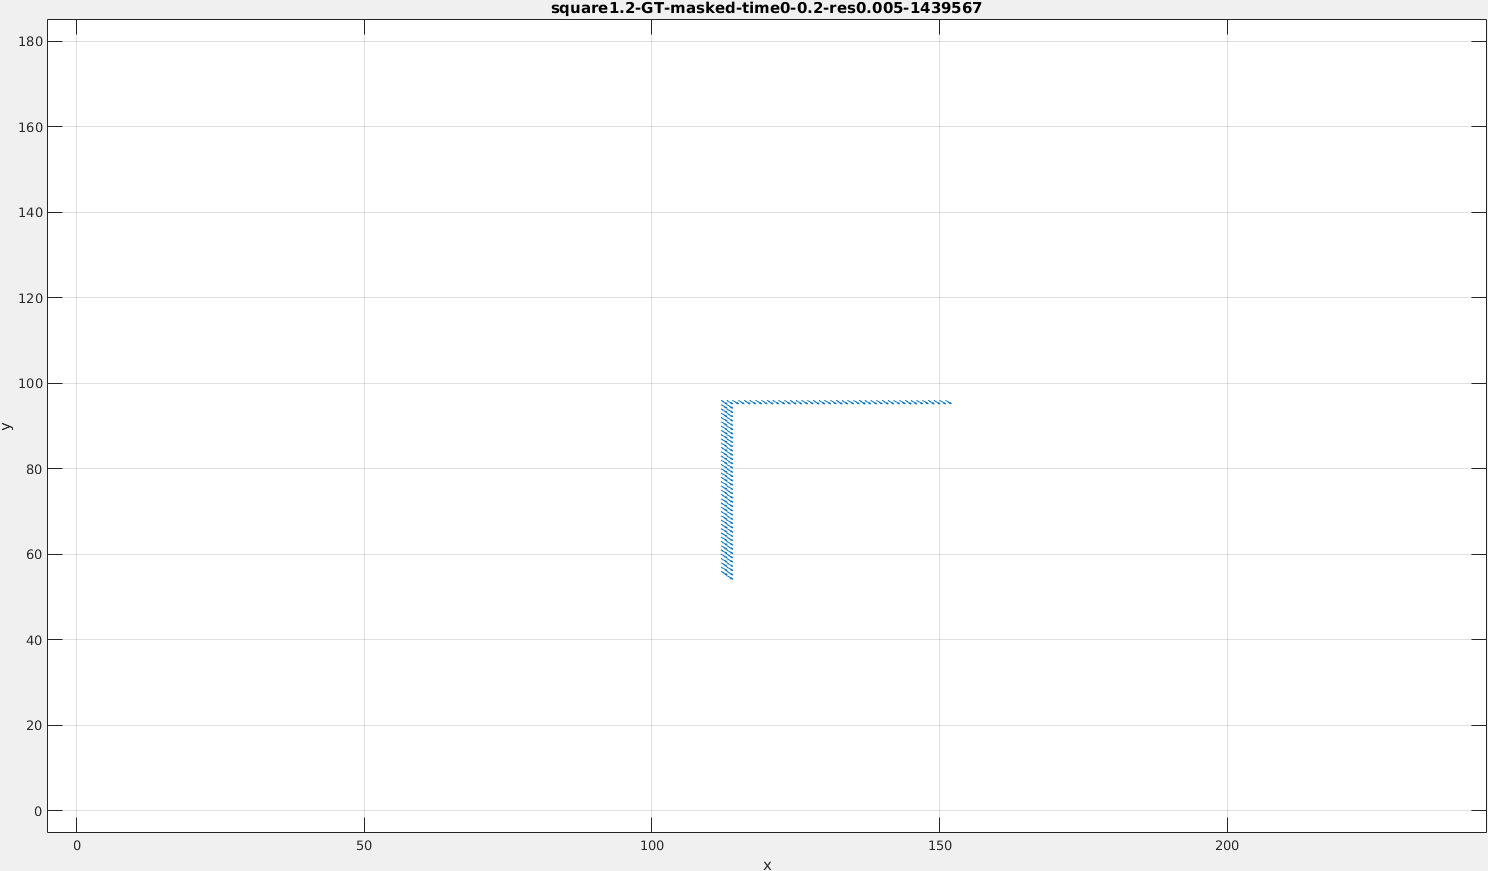
\includegraphics[height=.6\linewidth]{figs/square12/square12-GT-masked-1.png}
  \caption{}
\end{subfigure}
\begin{subfigure}{.45\textwidth}
  \centering
  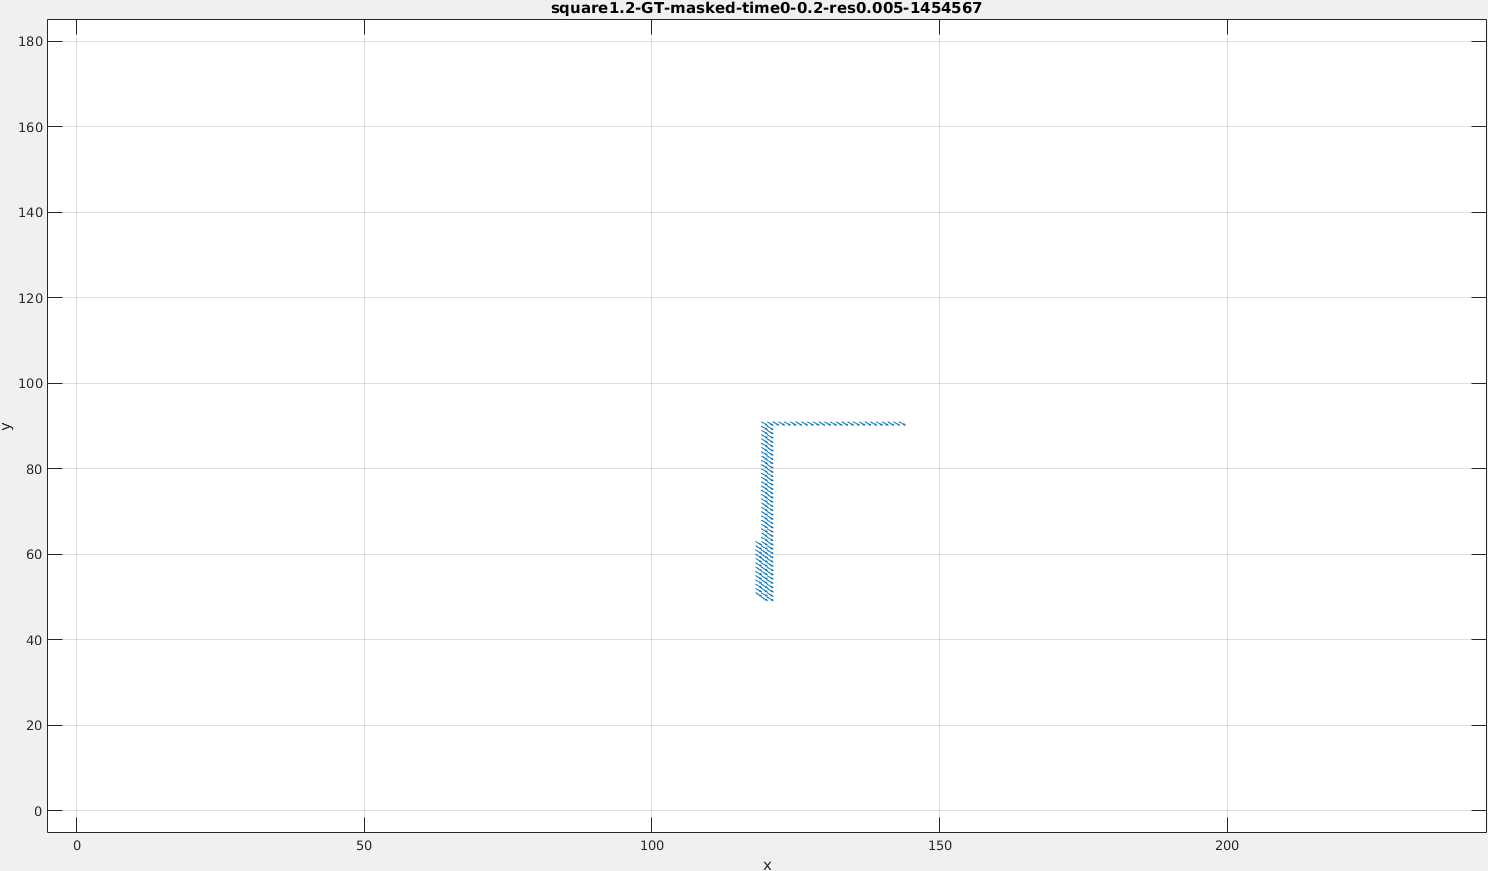
\includegraphics[height=.6\linewidth]{figs/square12/square12-GT-masked-2.png}
  \caption{}
\end{subfigure}
\caption[Fourth scene: Synthetic data of a linearly moving square.]{Fourth scene: Synthetic data of a linearly moving square.
Figures (a) and (b) show the computed optical flow for the scene at two time steps. The masked flow fields are shown in Figures (c) and (d).
The corresponding ground truth is shown in Figures (e) and (f). Applying the same mask leads to Figures (g) and (h).
Due to the synthetic nature of the data, all pixels of the outer edges moved simultaneously.
This leads to our algorithm failing to recognize the edges at all.
The effects of the aperture problem are visible a the right and bottom corner of the edges in Figures (a) and (b).
}
\label{fig:app_square12-snapshots}
\end{figure}
	 
	\begin{figure}[tb]
\centering
\begin{subfigure}{.45\textwidth}
  \centering
  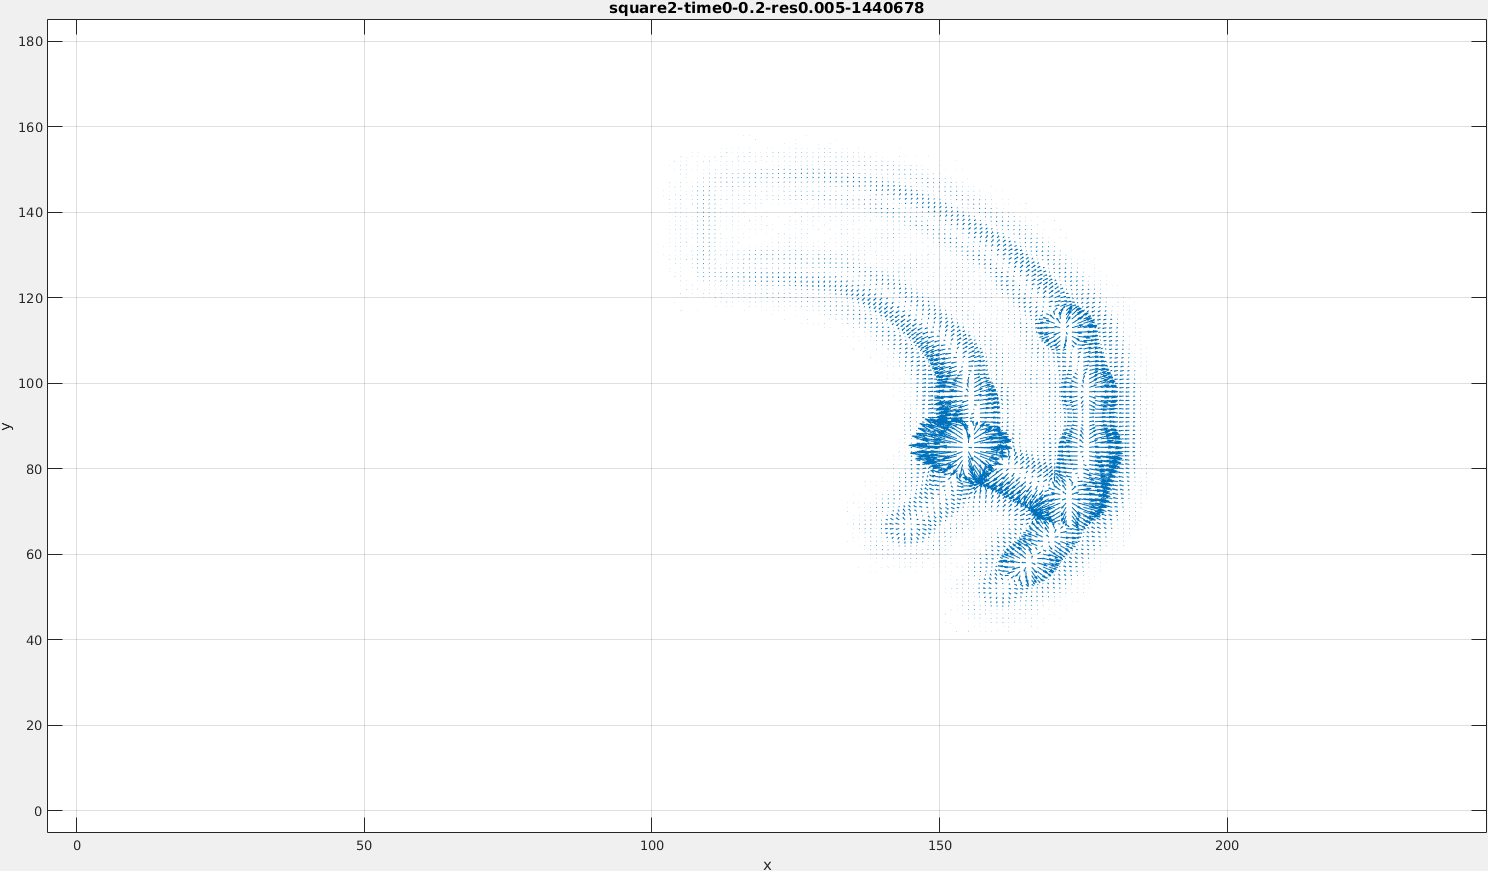
\includegraphics[height=.6\linewidth]{figs/square2/square2-1.png}
  \caption{}
\end{subfigure}
\begin{subfigure}{.45\textwidth}
  \centering
  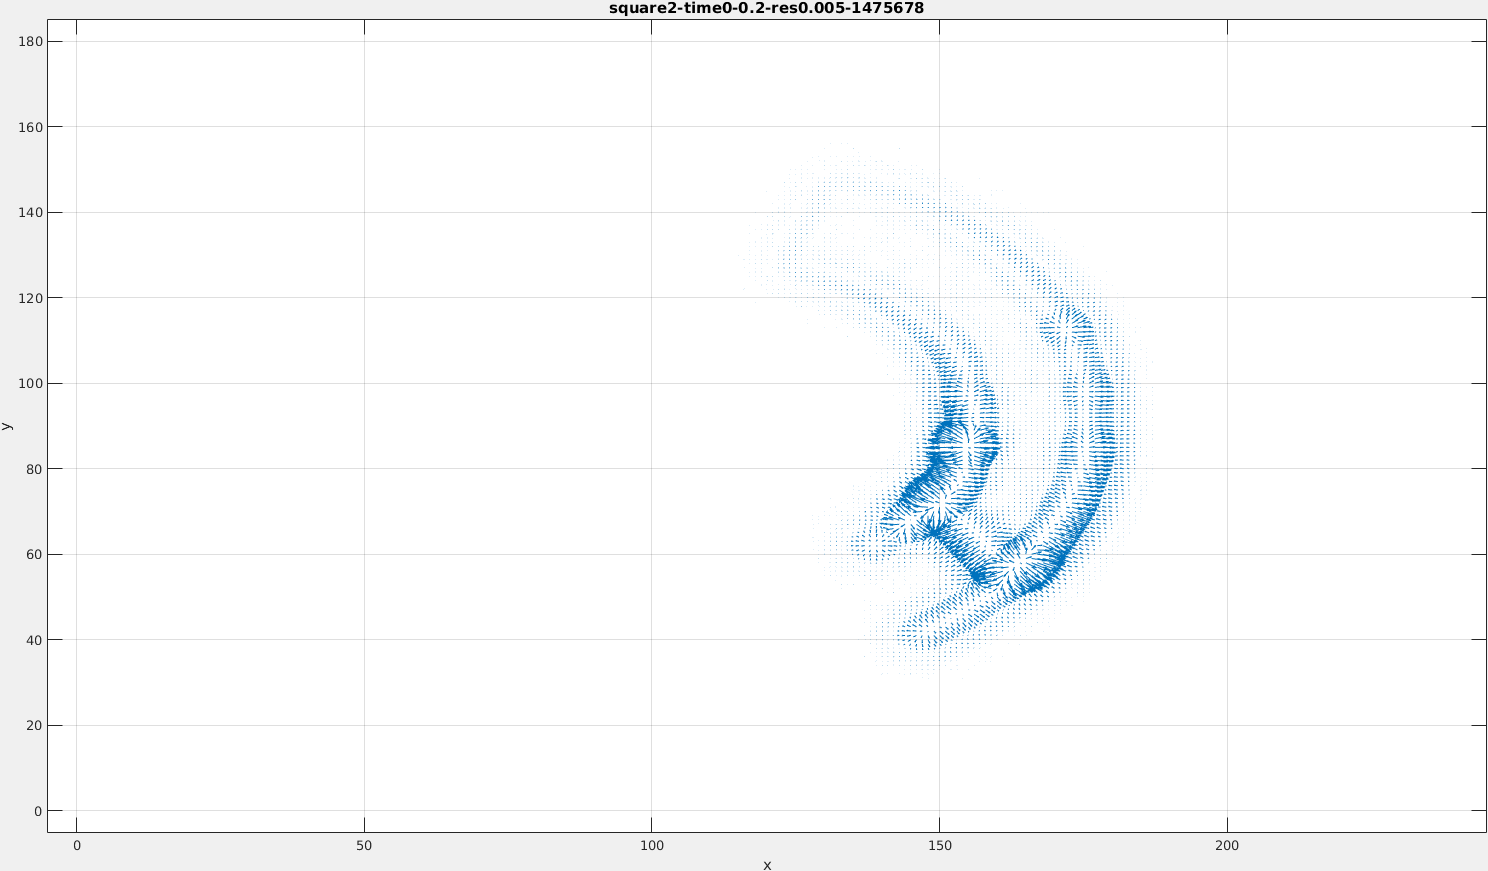
\includegraphics[height=.6\linewidth]{figs/square2/square2-2.png}
  \caption{}
\end{subfigure}
\begin{subfigure}{.45\textwidth}
  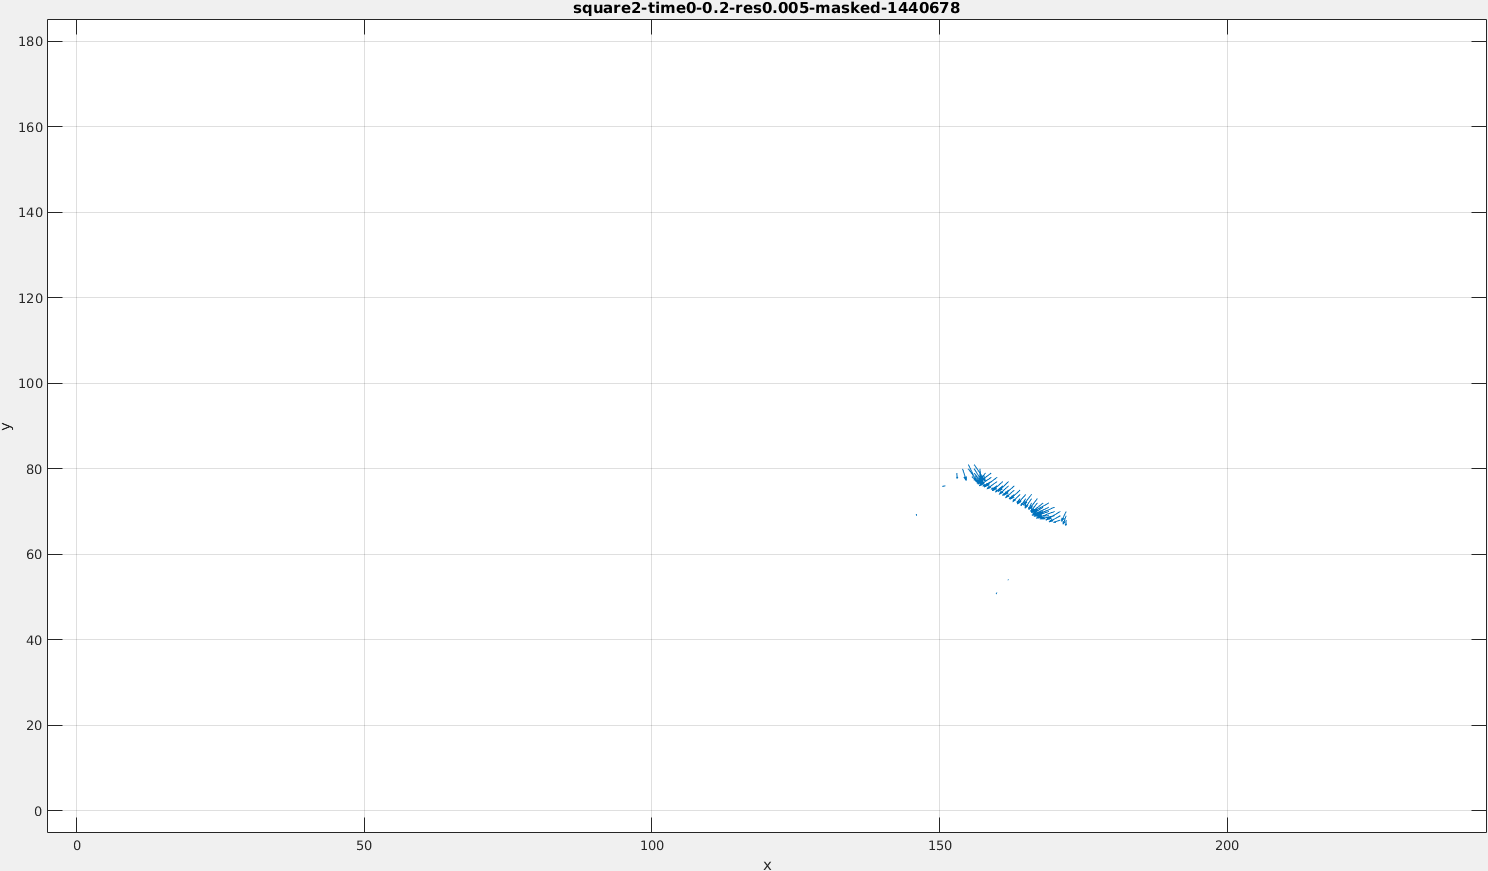
\includegraphics[height=.6\linewidth]{figs/square2/square2-masked-1.png}
  \caption{}
\end{subfigure}
\begin{subfigure}{.45\textwidth}
  \centering
  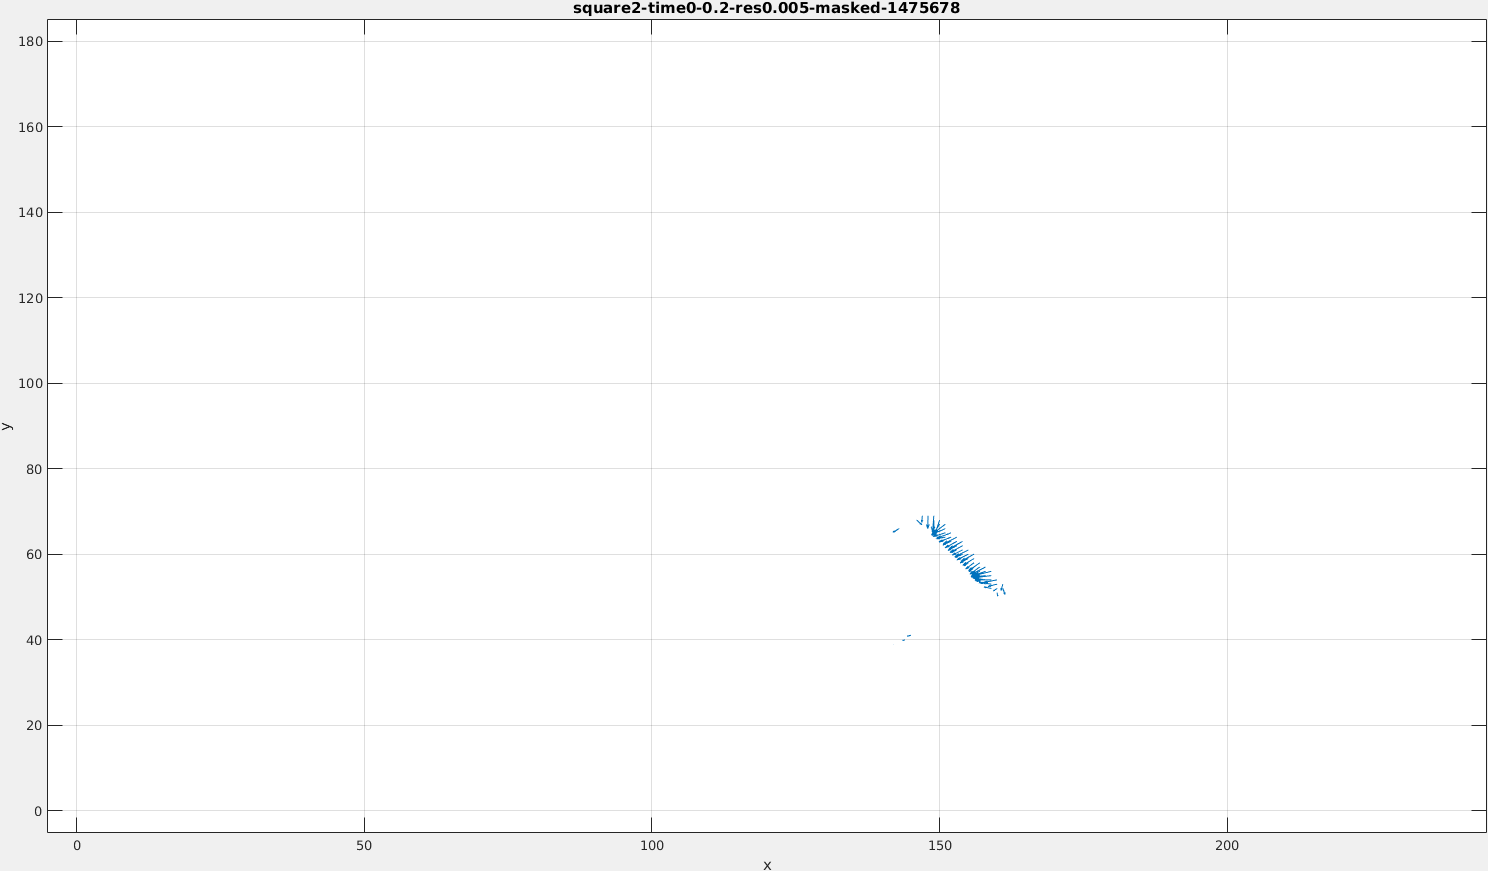
\includegraphics[height=.6\linewidth]{figs/square2/square2-masked-2.png}
  \caption{}
\end{subfigure}
\begin{subfigure}{.45\textwidth}
  \centering
  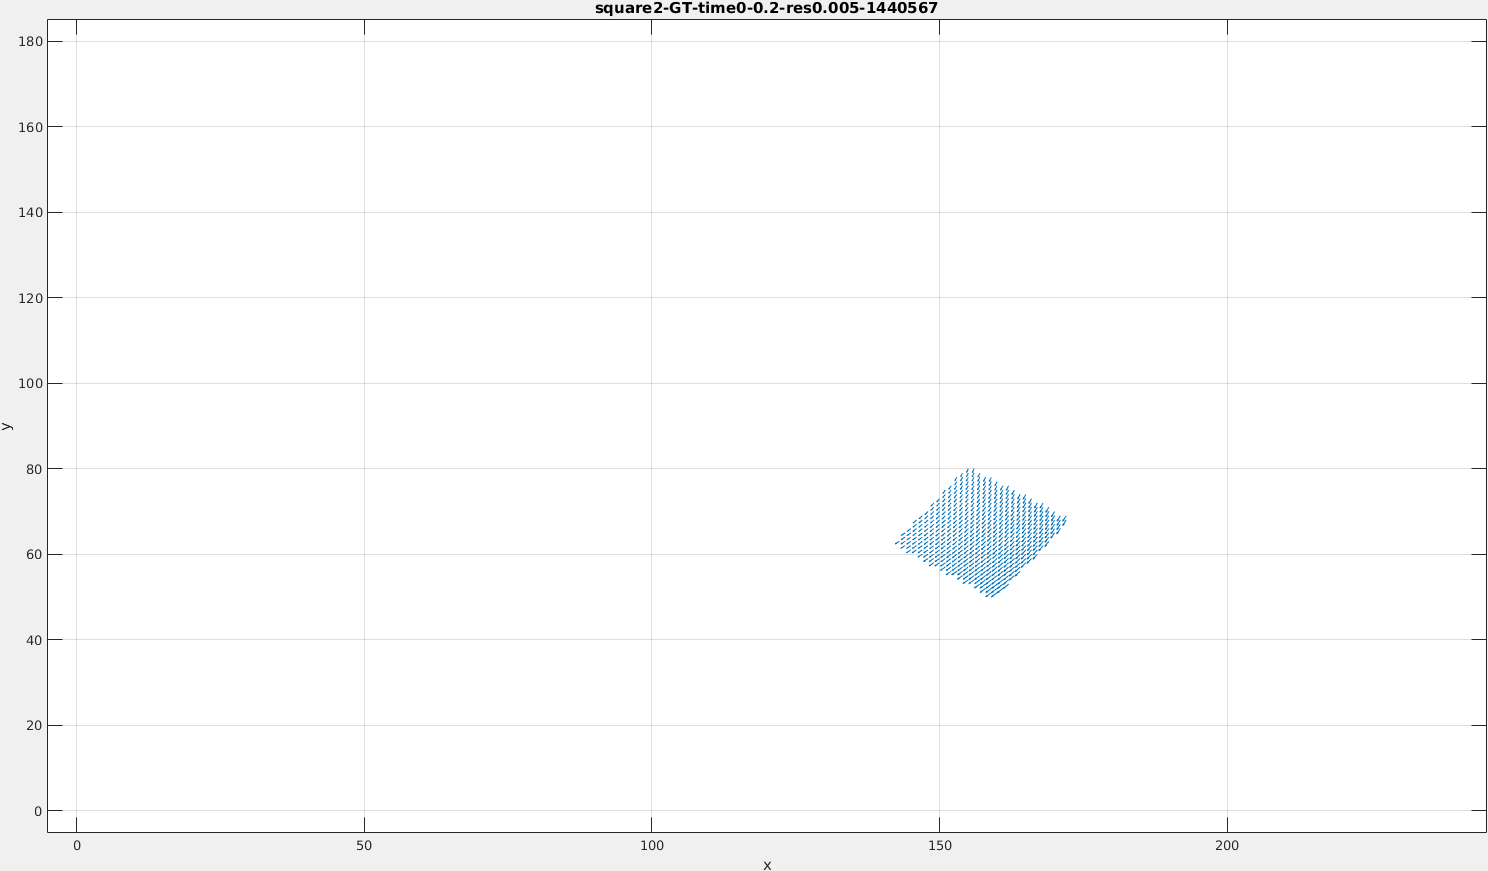
\includegraphics[height=.6\linewidth]{figs/square2/square2-GT-1.png}
  \caption{}
\end{subfigure}
\begin{subfigure}{.45\textwidth}
  \centering
  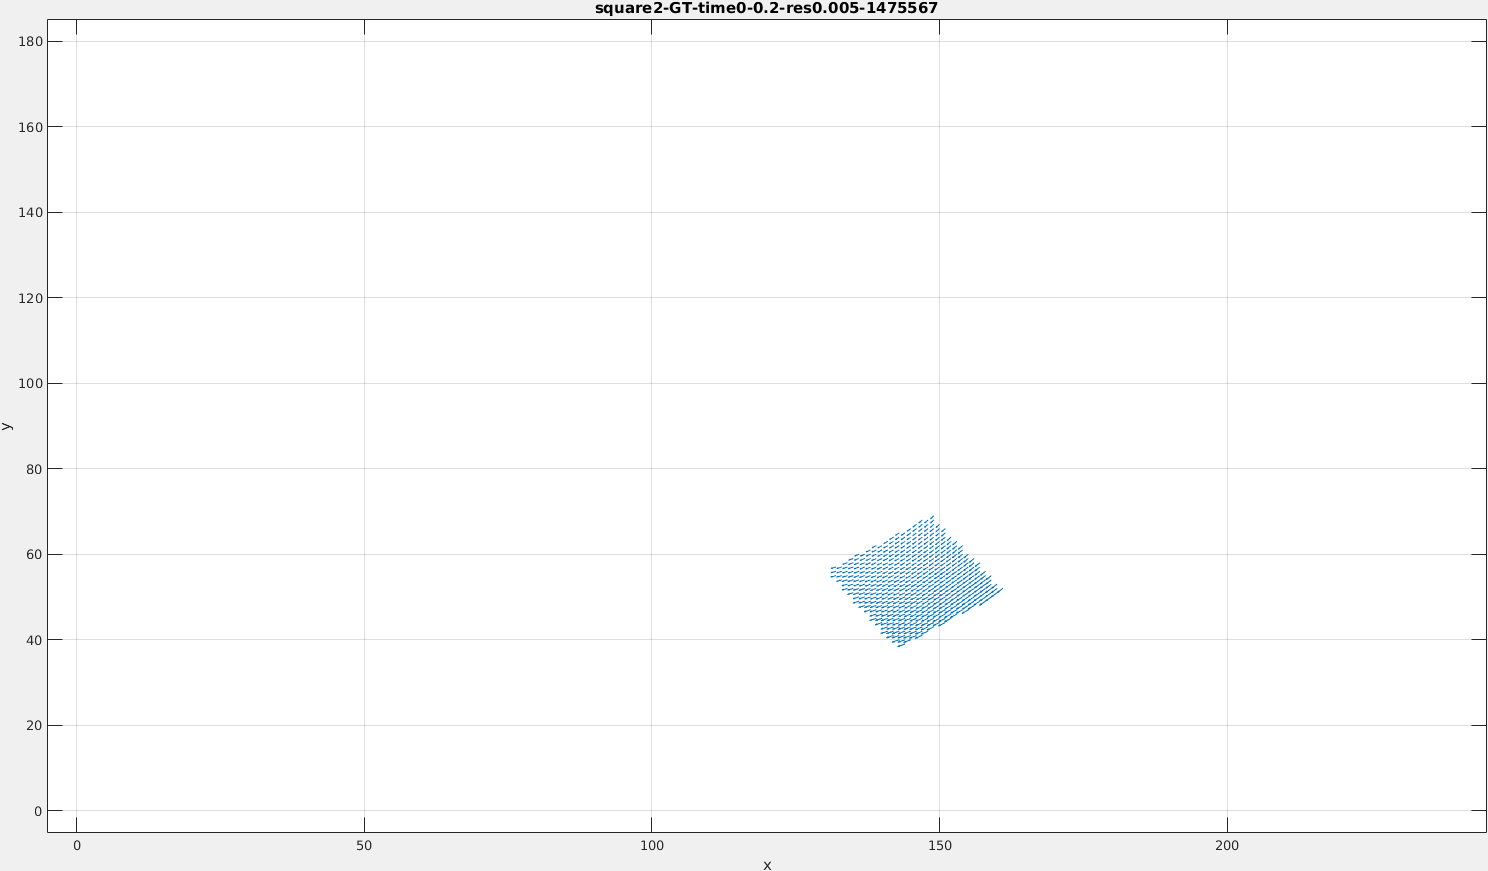
\includegraphics[height=.6\linewidth]{figs/square2/square2-GT-2.png}
  \caption{}
\end{subfigure}
\begin{subfigure}{.45\textwidth}
  \centering
  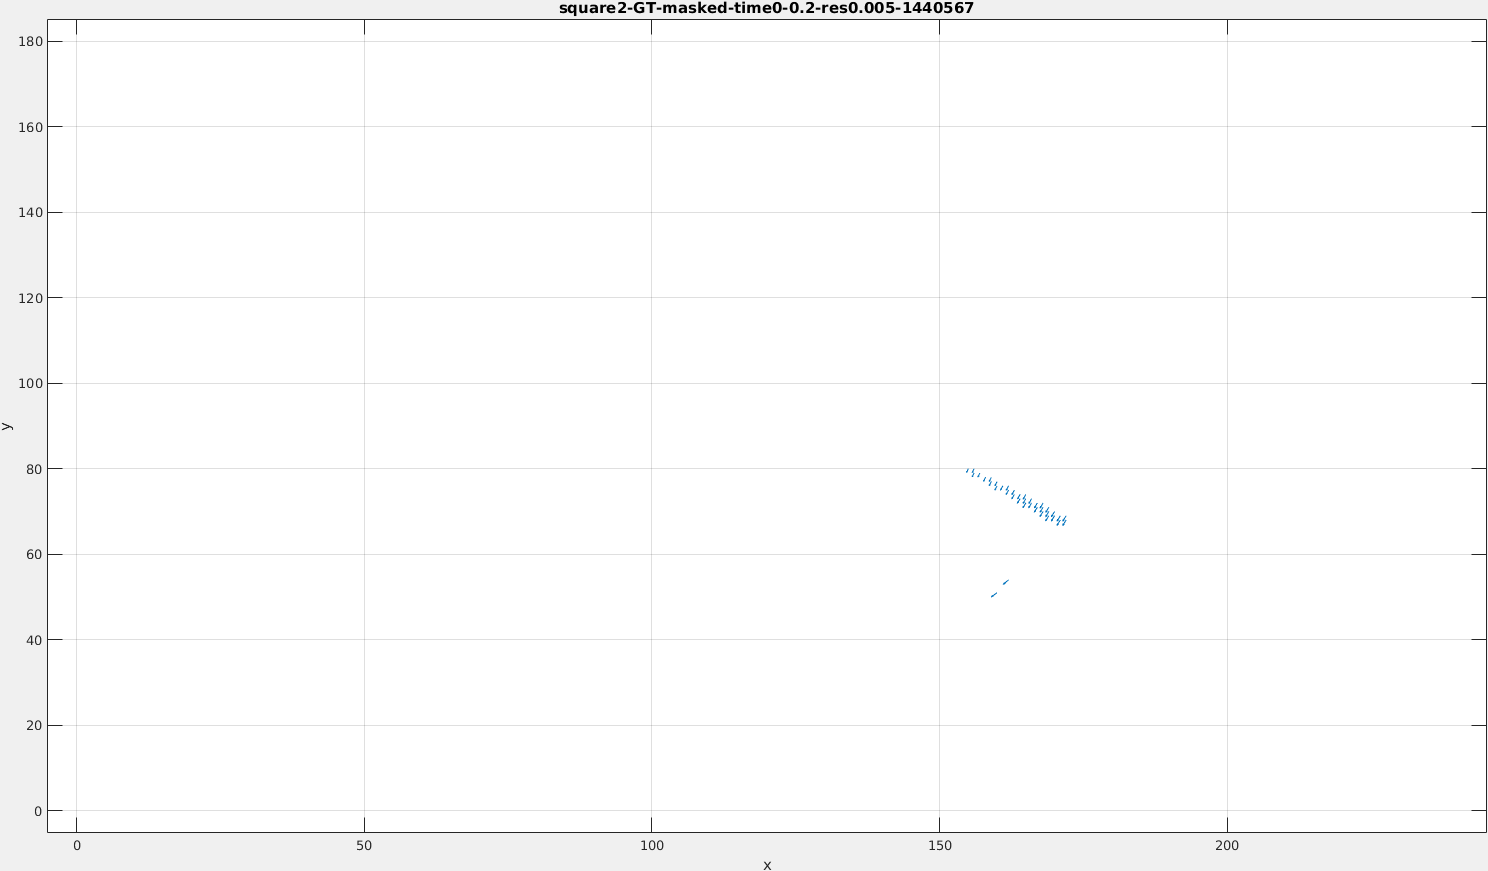
\includegraphics[height=.6\linewidth]{figs/square2/square2-GT-masked-1.png}
  \caption{}
\end{subfigure}
\begin{subfigure}{.45\textwidth}
  \centering
  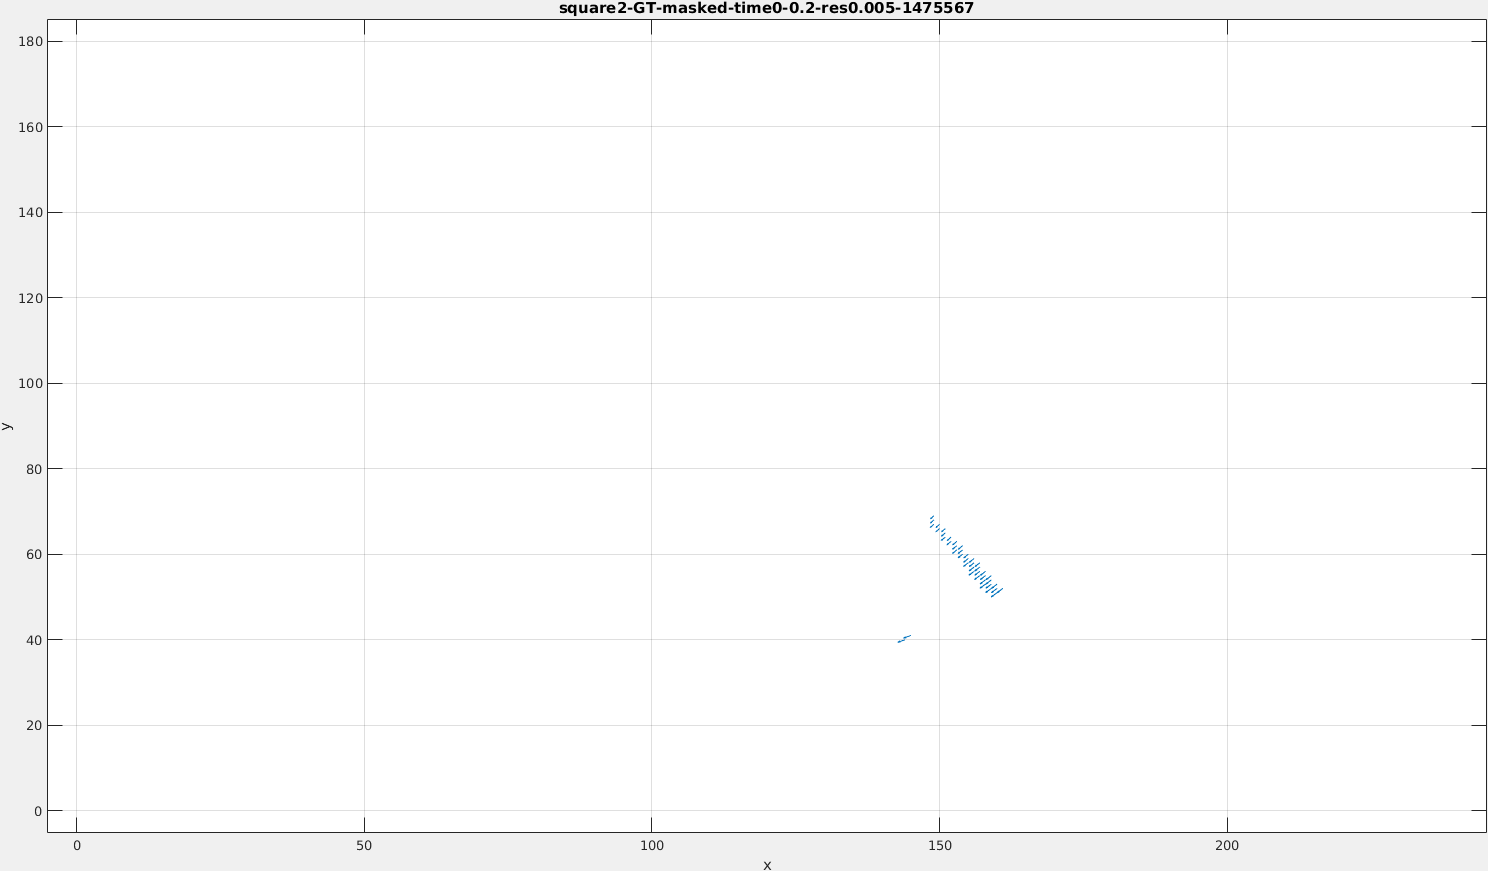
\includegraphics[height=.6\linewidth]{figs/square2/square2-GT-masked-2.png}
  \caption{}
\end{subfigure}
\caption[Fifth scene: Synthetic data of a circularly moving square.]{Fifth scene: Synthetic data of a circularly moving square.
Figures (a) and (b) show the computed optical flow for the scene at two time steps. The masked flow fields are shown in Figures (c) and (d).
The corresponding ground truth is shown in Figures (e) and (f). Applying the same mask leads to Figures (g) and (h)}
\label{fig:app_square2-snapshots}
\end{figure} 
	 
\begin{figure}[tb]
\centering
\begin{subfigure}{.45\textwidth}
  \centering
  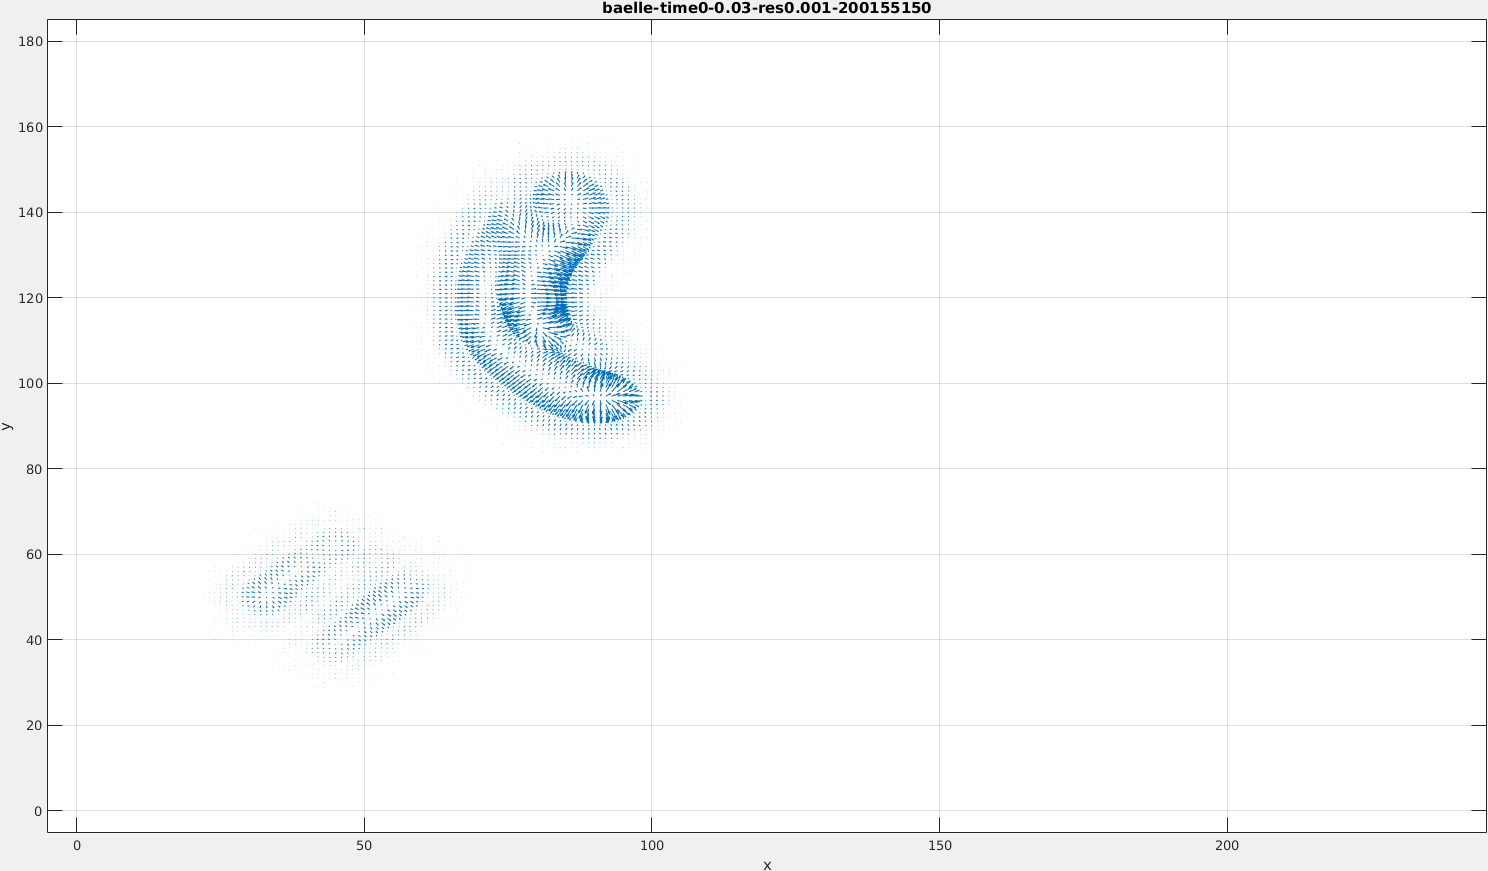
\includegraphics[height=.6\linewidth]{figs/baelle/baelle-1.png}
  \caption{}
%\label{fig:baelle-snapshots1}
\end{subfigure}
\begin{subfigure}{.45\textwidth}
  \centering
  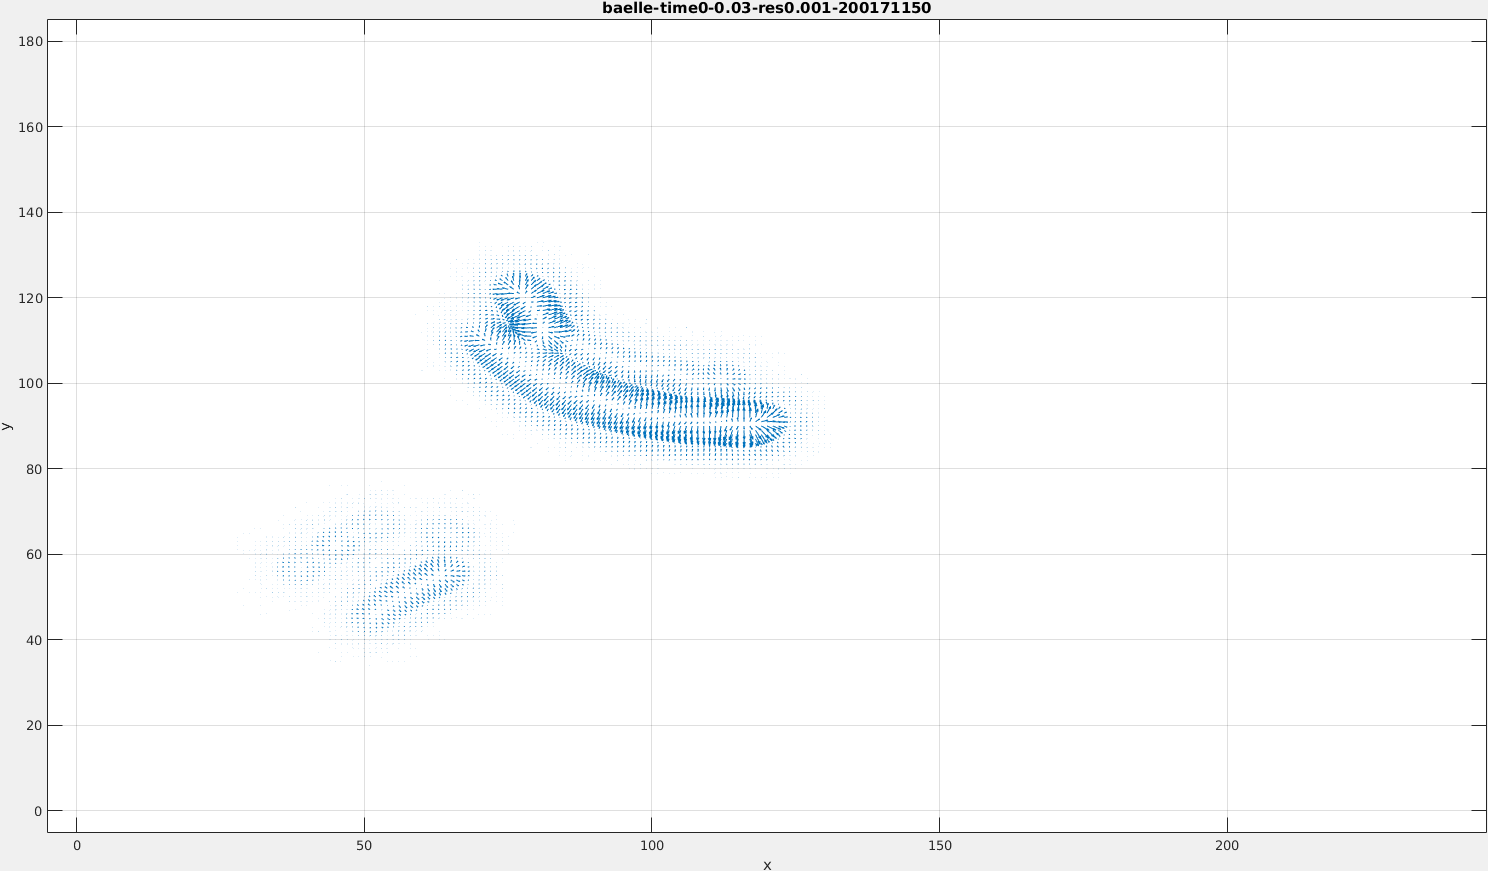
\includegraphics[height=.6\linewidth]{figs/baelle/baelle-2.png}
  \caption{}
%  \label{fig:baelle-snapshots2}
\end{subfigure}
\begin{subfigure}{.45\textwidth}
  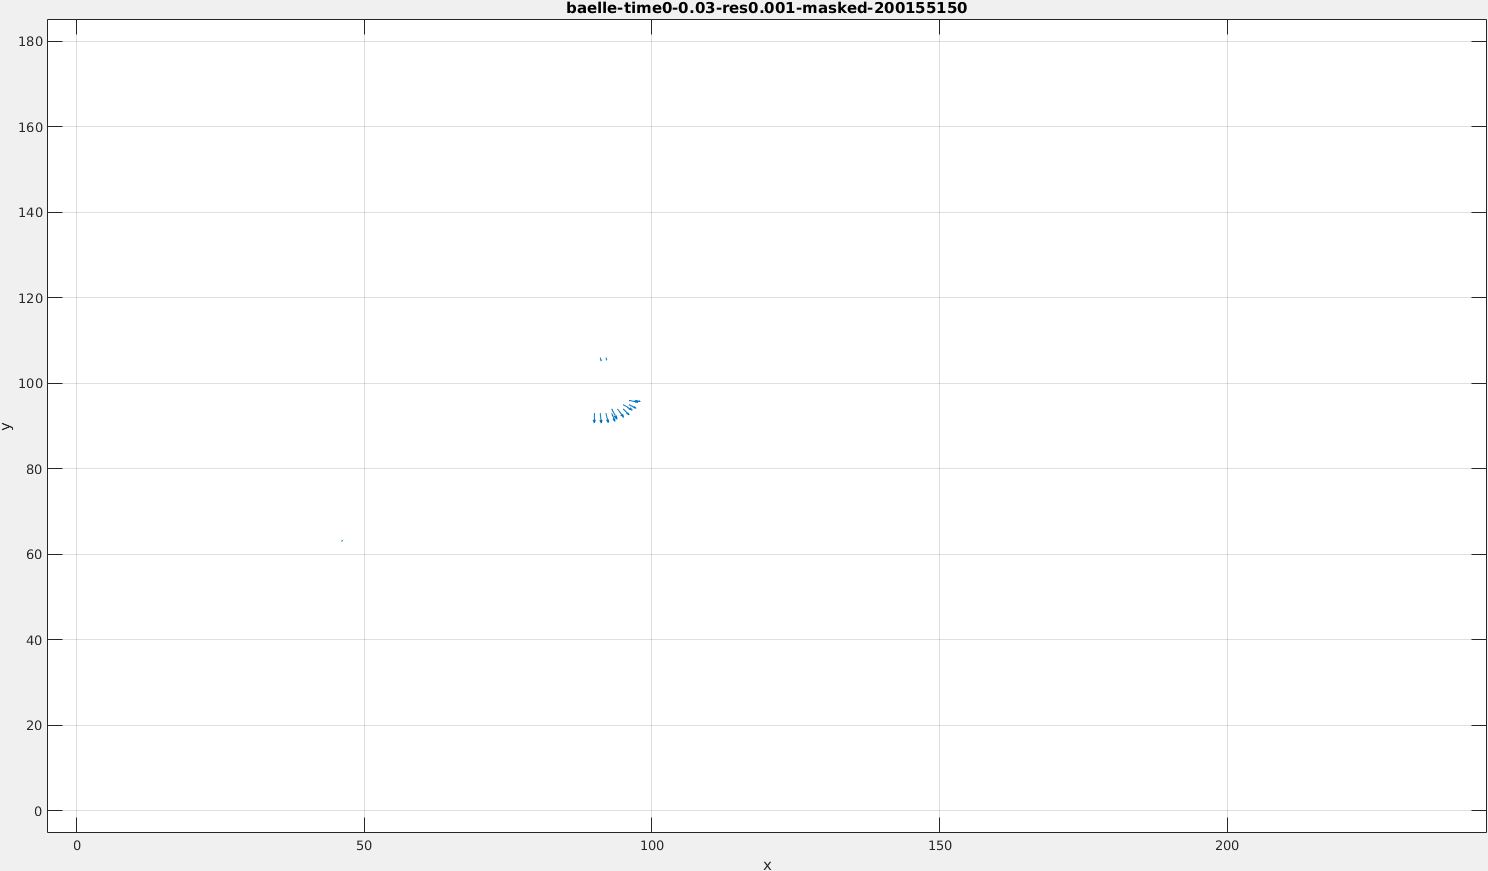
\includegraphics[height=.6\linewidth]{figs/baelle/baelle-masked-1.png}
  \caption{}
\end{subfigure}
\begin{subfigure}{.45\textwidth}
  \centering
  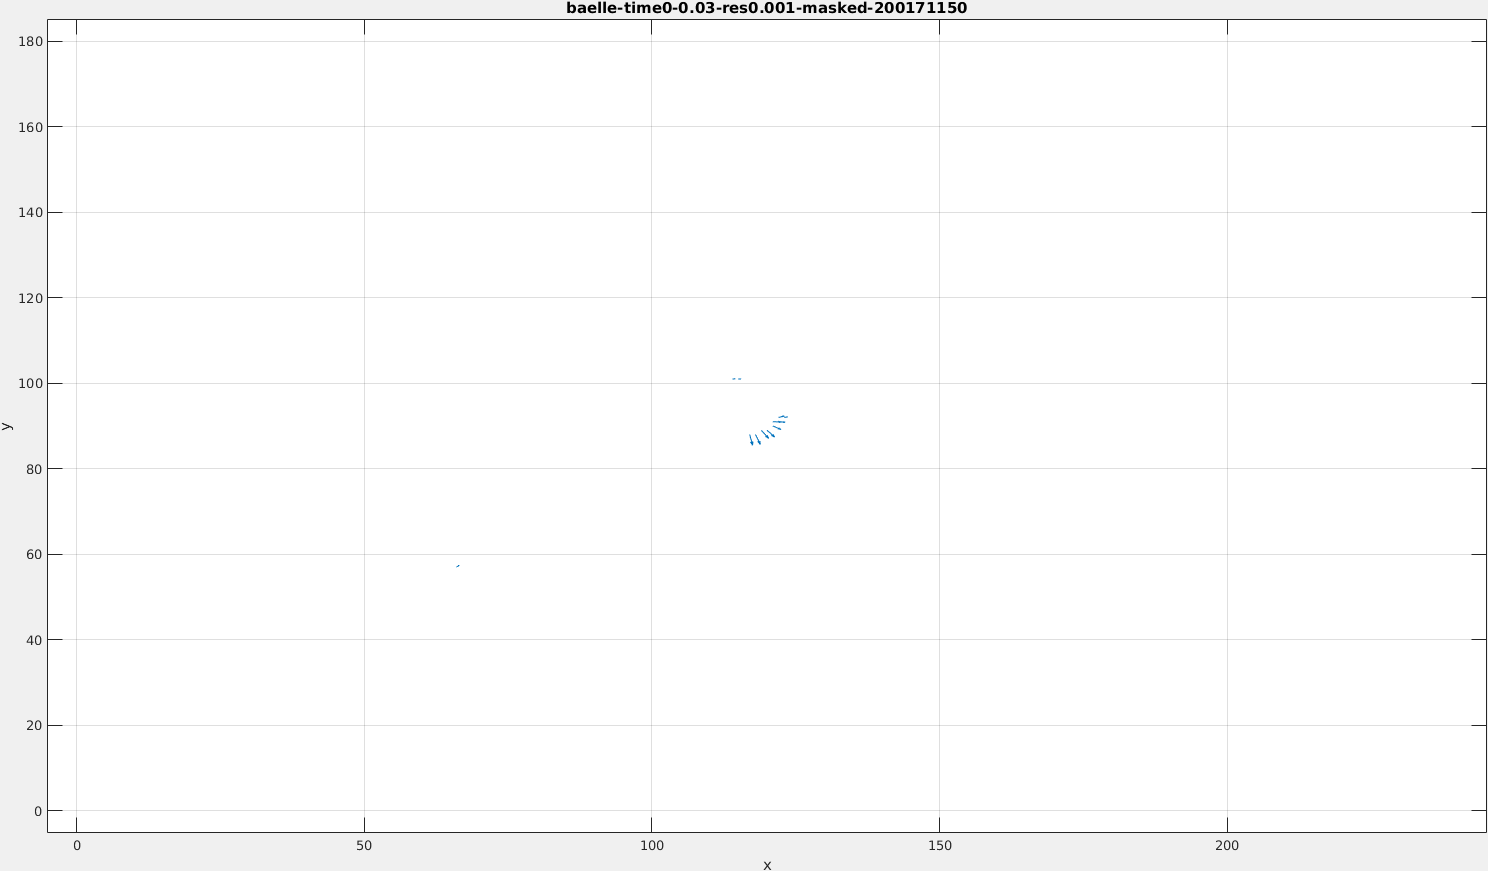
\includegraphics[height=.6\linewidth]{figs/baelle/baelle-masked-2.png}
  \caption{}
\end{subfigure}
\begin{subfigure}{.45\textwidth}
  \centering
  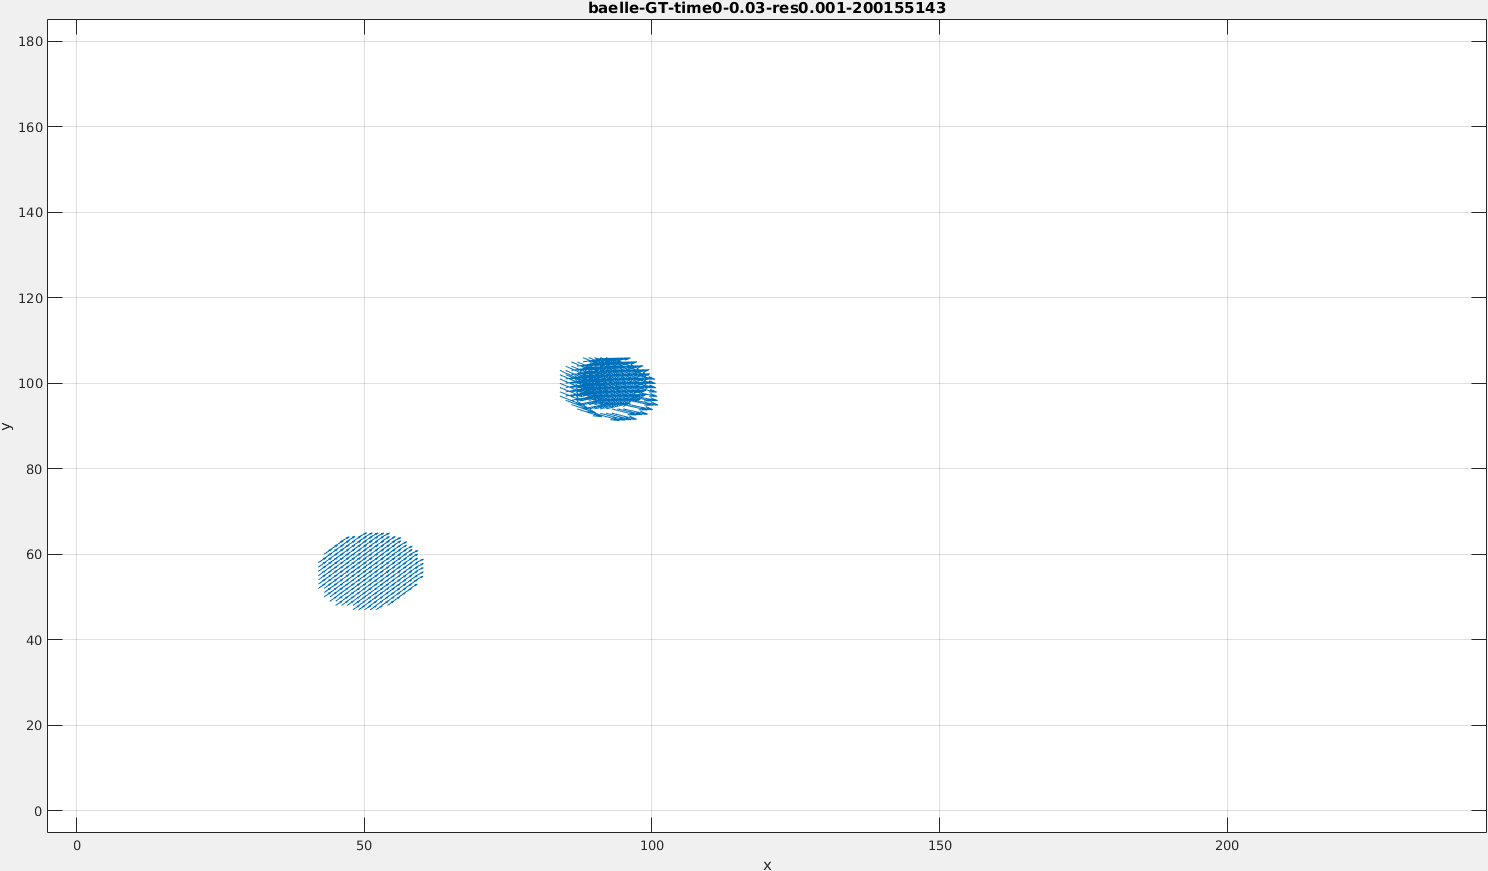
\includegraphics[height=.6\linewidth]{figs/baelle/baelle-GT-1.png}
  \caption{}
\end{subfigure}
\begin{subfigure}{.45\textwidth}
  \centering
  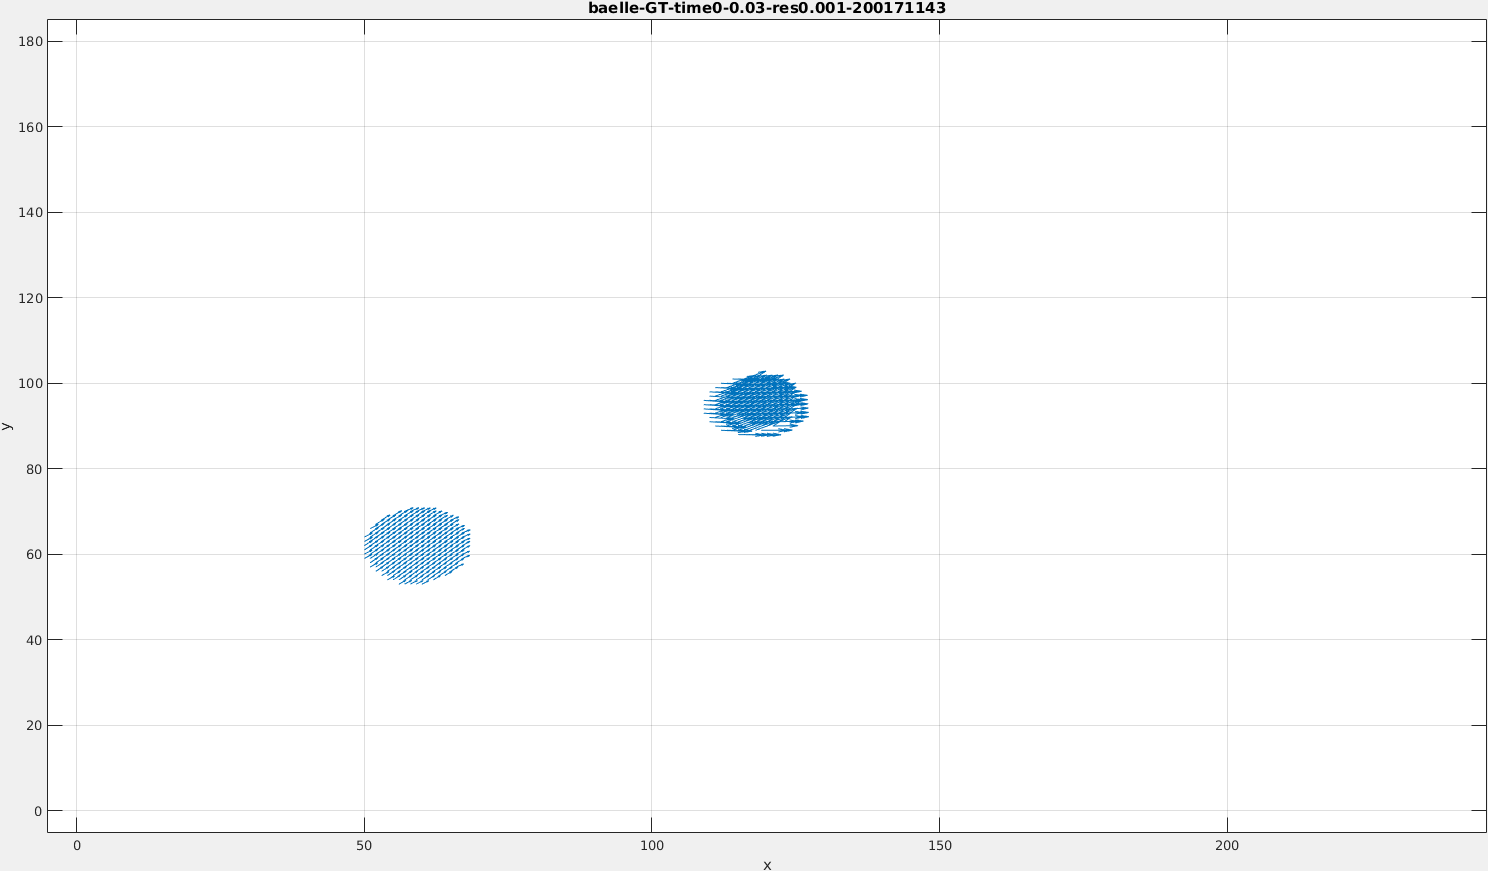
\includegraphics[height=.6\linewidth]{figs/baelle/baelle-GT-2.png}
  \caption{}
\end{subfigure}
\begin{subfigure}{.45\textwidth}
  \centering
  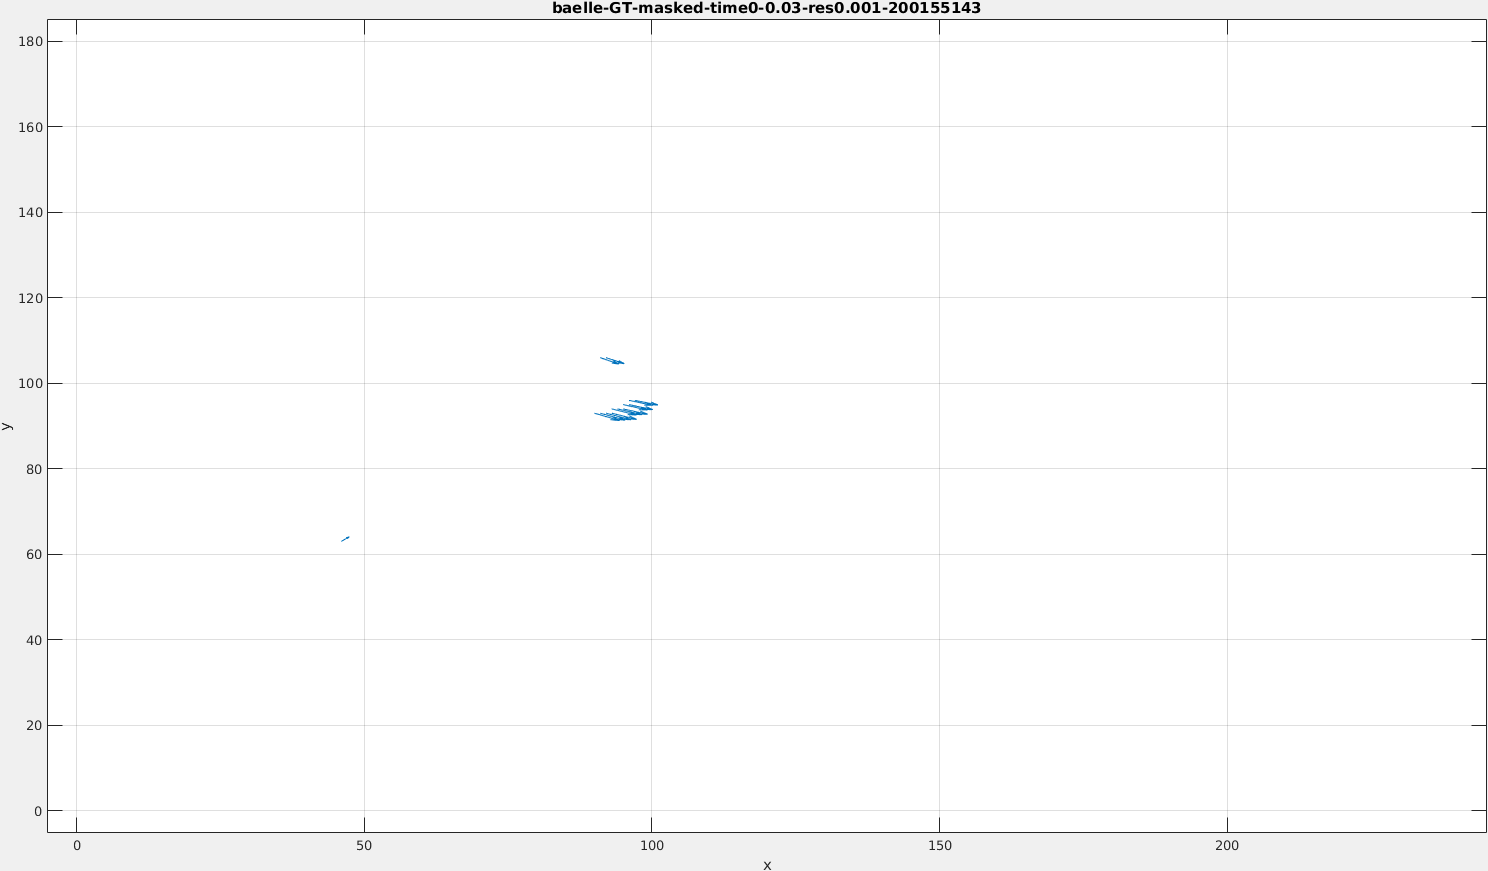
\includegraphics[height=.6\linewidth]{figs/baelle/baelle-GT-masked-1.png}
  \caption{}
\end{subfigure}
\begin{subfigure}{.45\textwidth}
  \centering
  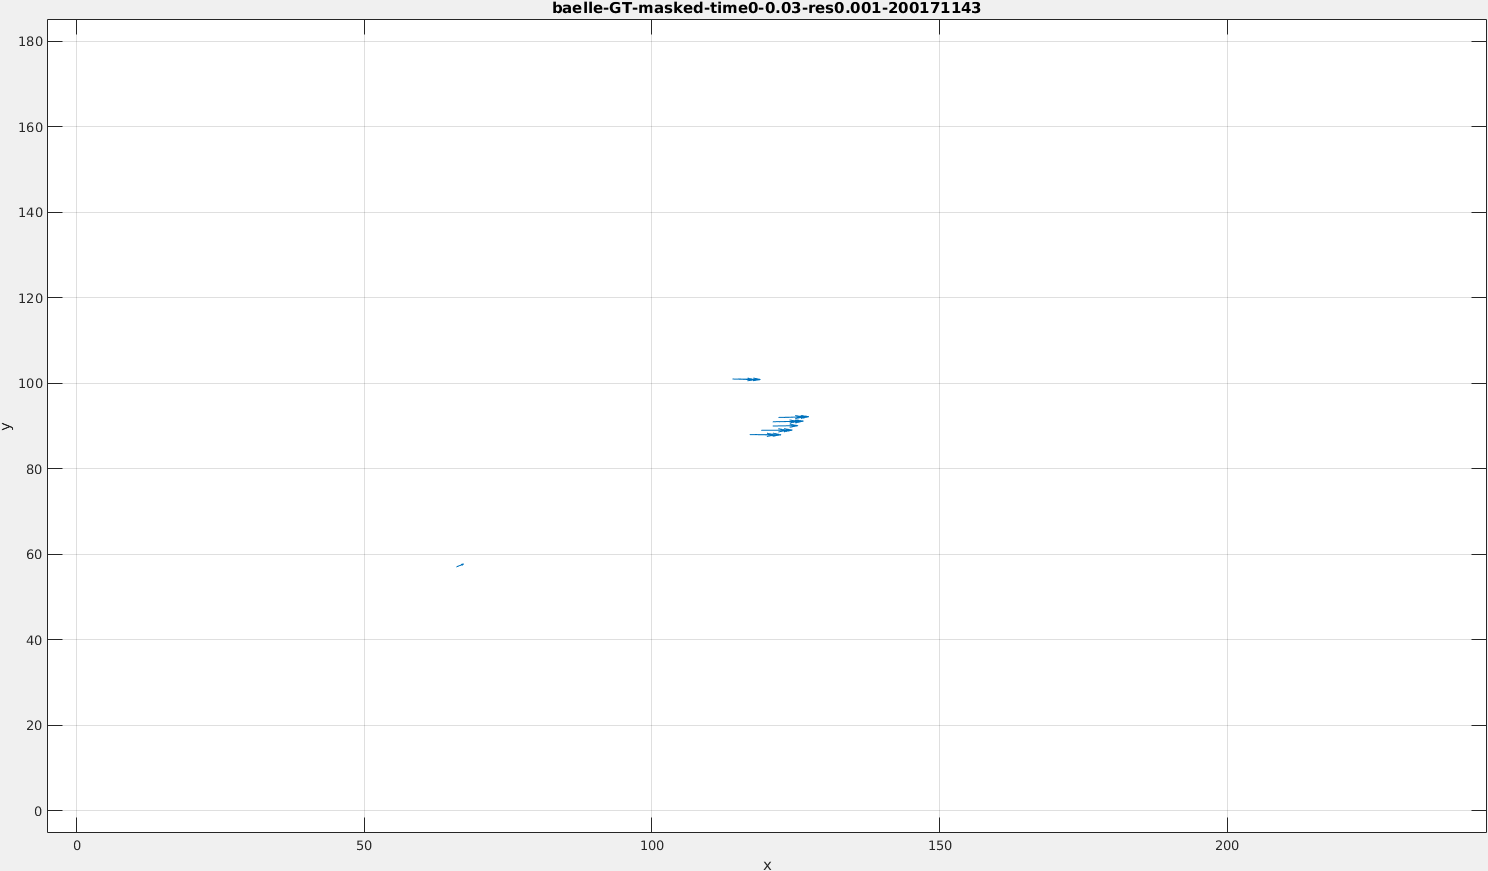
\includegraphics[height=.6\linewidth]{figs/baelle/baelle-GT-masked-2.png}
  \caption{}
\end{subfigure}
\caption[Sixth scene: Synthetic data of two balls moving through the scene.]{Sixth scene: Synthetic data of two balls moving through the scene.
Figures (a) and (b) show the computed optical flow for the scene at two time steps. The masked flow fields are shown in Figures (c) and (d).
The corresponding ground truth is shown in Figures (e) and (f). Applying the same mask leads to Figures (g) and (h).
Due to a shading effect, two edges are detected for the upper sphere by the algorithm (a)(b).}
\label{fig:app_baelle-snapshots}
\end{figure}
	 
	 
\end{appendix}
